\documentclass[%
pdf,
%nocolorBG,
colorBG,
slideColor,
%slideBW,
%draft,
%frames
%azure
%contemporain
%nuancegris
%troispoints
%lignesbleues
%darkblue
%alienglow
%autumn
]{prosper}
\usepackage{pifont, amsmath, multicol}
%\usepackage{floatflt, wrapfig,subfigure}
%\usepackage{wrapfig}
%\usepackage{floatflt}
\usepackage{color}
\usepackage{epsfig}
\usepackage{pifont}
\usepackage[T1]{fontenc}
\usepackage[latin1]{inputenc}
\def\QuotS#1#2{\leavevmode\kern-.0em\raise.2ex\hbox{$#1$}\kern-.1em/\kern-.1em\lower.25ex\hbox{$#2$}}


%\usepackage[francais]{babel}
%\defÂ«{\og\ignorespaces}%
%\defÂ»{{\fg}}%
\newcommand{\spacer}{\rule[-3mm]{0mm}{8mm}}
\newtheorem{theorem}{Theorem}
\newtheorem{definition}[theorem]{Definition}

\newcommand{\RR}{\ensuremath{\mathbb{R}}}
\newcommand{\NN}{\ensuremath{\mathbb{N}}}
\newcommand{\QQ}{\ensuremath{\mathbb{Q}}}
\newcommand{\CC}{\ensuremath{\mathbb{C}}}
\newcommand{\ZZ}{\ensuremath{\mathbb{Z}}}
\newcommand{\TT}{\ensuremath{\mathbb{T}}}

\def\QuotS#1#2{\leavevmode\kern-.0em\raise.2ex\hbox{$#1$}\kern-.1em/\kern-.1em\lower.25ex\hbox{$#2$}}


\title{\Huge \textcolor{blue}{Fullerenes: applications and generalizations}}



\author{
\textcolor{red}{\Large Michel Deza}\\[2mm]
\textcolor{red}{\large Ecole Normale Superieure, Paris}\\[2mm]
\textcolor{red}{\Large Mathieu Dutour Sikiri\'c}\\[2mm]
\textcolor{red}{\large Rudjer Bo\u skovi\'c Institute, Zagreb, and ISM, Tokyo}
}


\slideCaption{}

\date{}



\begin{document}
\maketitle




\begin{slide}{}
\begin{center}
{\Huge 
\begin{tabular*}{5cm}{c}
\\[-0.5cm]
\textcolor{blue}{I. }\textcolor{red}{General}\\
\textcolor{red}{setting}
\end{tabular*}
}
\end{center}
\end{slide}



\begin{slide}{Definition}
A \textcolor{red}{fullerene} $F_n$ is a \textcolor{blue}{simple polyhedron} (putative carbon molecule) whose $n$ vertices (carbon atoms) are arranged in $12$ \textcolor{blue}{pentagons} and $(\frac{n}{2}-10)$ \textcolor{blue}{hexagons}.

The $\frac{3}{2}n$ edges correspond to carbon-carbon bonds.
\begin{itemize}
\item $F_n$ exist for all even $n\geq 20$ except $n=22$.
\item $1,2,3,\dots,1812$ \textcolor{blue}{isomers} $F_n$ for $n=20$, $28$, $30$,\dots, $60$.
\item \textcolor{blue}{preferable} fullerenes, $C_n$, satisfy isolated pentagon rule.
\item $C_{60}(I_h)$, $C_{80}(I_h)$ are only \textcolor{blue}{icosahedral}
(i.e., with symmetry $I_h$ or $I$) fullerenes with $n \le 80$ vertices
\end{itemize}
\end{slide}




\begin{slide}{}
\begin{center}
\begin{minipage}[b]{5.5cm}
\centering
\resizebox{5.5cm}{!}{\includegraphics{DRAW/PS/C60.ps}}\par
buckminsterfullerene $C_{60}(I_h)$\\
{\em truncated icosahedron, \par
soccer ball}
\end{minipage}
\hspace{0.1cm}
\begin{minipage}[b]{5.5cm}
\centering
\resizebox{46mm}{!}{\includegraphics{DRAW/PS/F36.ps}}\par
$F_{36}(D_{6h})$\\
{\em elongated hexagonal barrel $F_{24}(D_{6d})$}
\end{minipage}
\end{center}
\end{slide}




\begin{slide}{}
\begin{center}
\begin{minipage}[b]{5.5cm}
\centering
\resizebox{46mm}{!}{\includegraphics{DRAW/PS/embeddingofF20.ps}}\par
Dodecahedron\par
$F_{20}(I_h)\rightarrow \frac{1}{2} H_{10}$\par
the \textcolor{red}{smallest} fullerene\par
\textcolor{white}{Bonjour}
\end{minipage}
\begin{minipage}[b]{5.5cm}
\centering
\resizebox{42mm}{!}{\rotatebox{0}{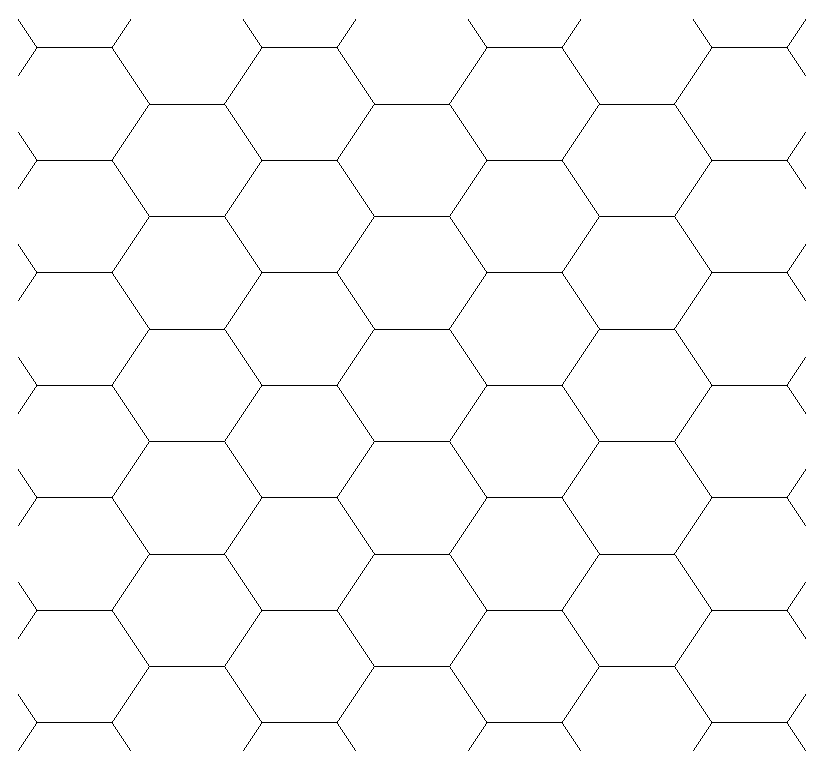
\includegraphics{FullPresPic/OtherReg2.eps}}}\par
Graphite lattice \par
$F_{\infty}\rightarrow Z_3$ \par
the \textcolor{red}{``largest''} (infinite) fullerene
\end{minipage}
\end{center}
\end{slide}




\begin{slide}{Small fullerenes}
\begin{center}
\begin{minipage}[b]{2.7cm}
\centering
\resizebox{25mm}{!}{\includegraphics{PictureAppli/F2sec.eps}}\par
24, $D_{6d}$
\end{minipage}
\begin{minipage}[b]{2.7cm}
\centering
\resizebox{25mm}{!}{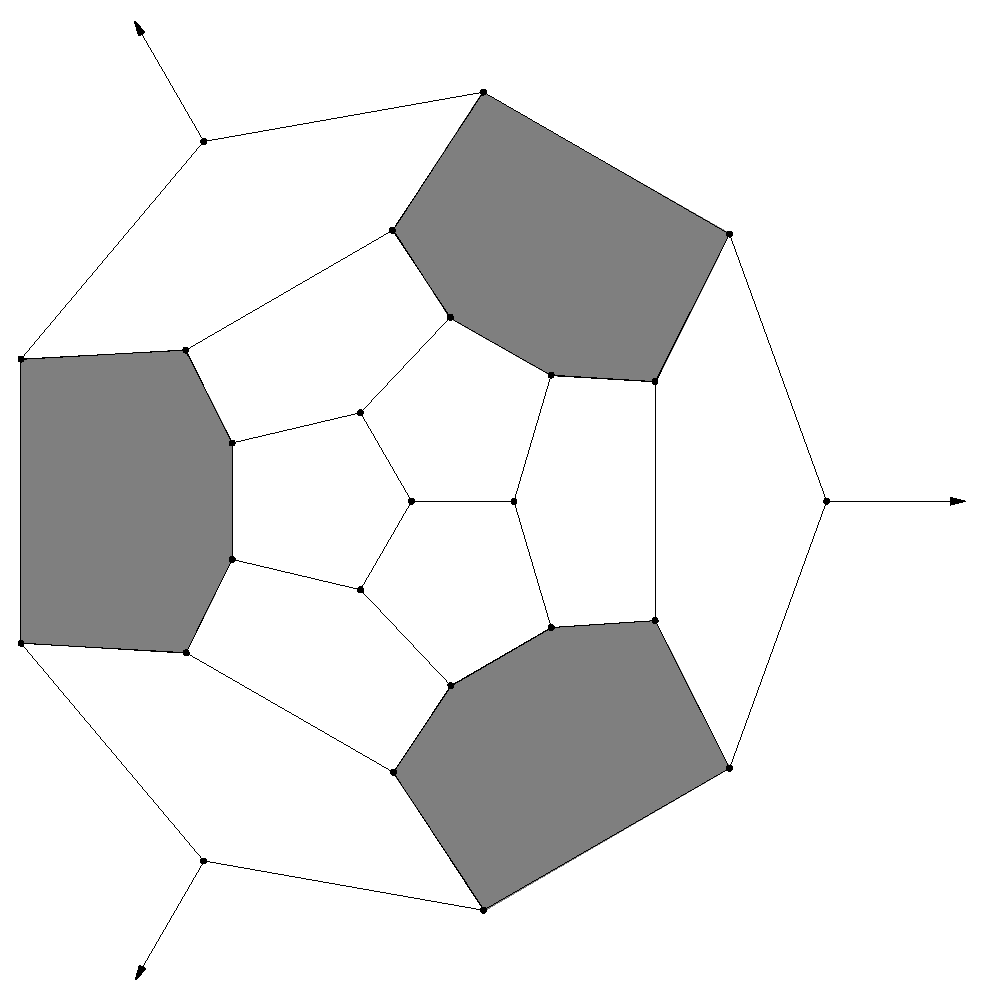
\includegraphics{FullPresPic/Picture2.eps}}\par
26, $D_{3h}$
\end{minipage}
\begin{minipage}[b]{2.7cm}
\centering
\resizebox{25mm}{!}{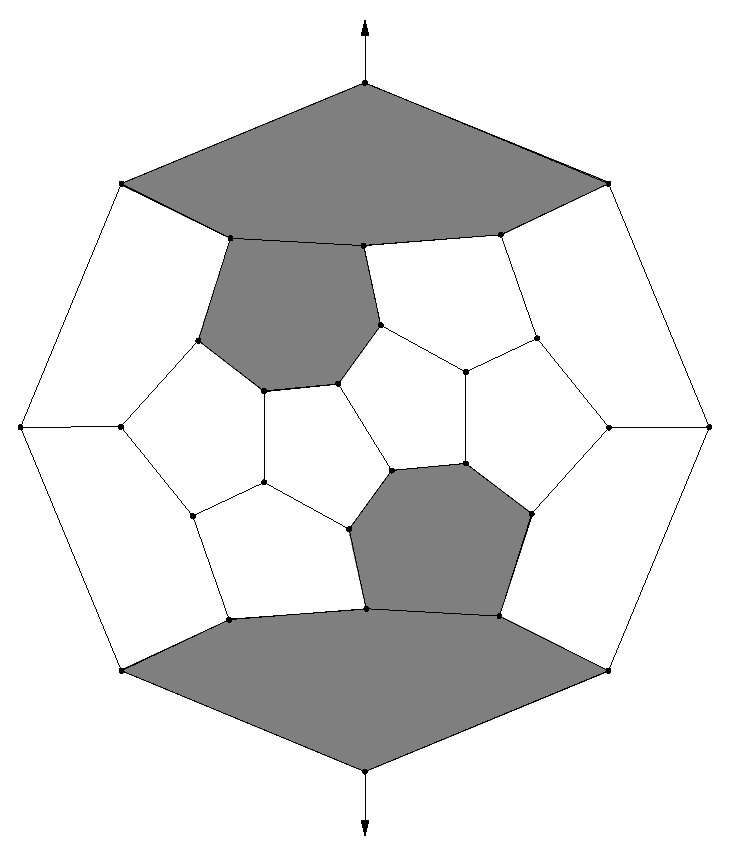
\includegraphics{FullPresPic/Picture3.eps}}\par
28, $D_{2}$
\end{minipage}
\begin{minipage}[b]{2.7cm}
\centering
\resizebox{25mm}{!}{\includegraphics{PictureAppli/F4sec.eps}}\par
28, $T_{d}$
\end{minipage}
\begin{minipage}[b]{2.7cm}
\centering
\resizebox{25mm}{!}{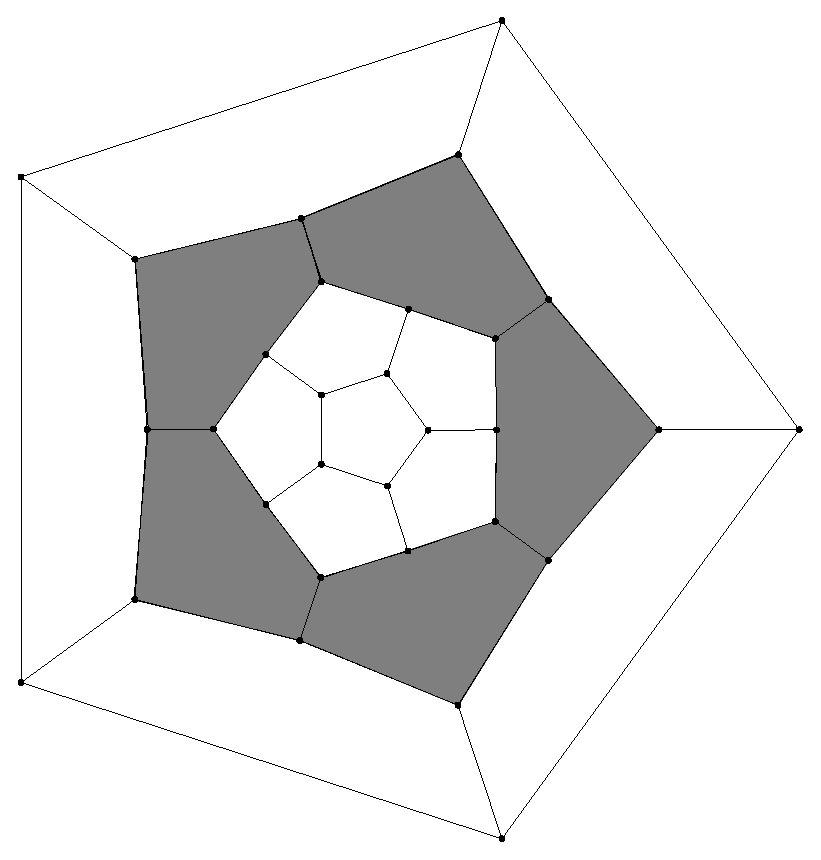
\includegraphics{FullPresPic/Picture5.eps}}\par
30, $D_{5h}$
\end{minipage}
\begin{minipage}[b]{2.7cm}
\centering
\resizebox{25mm}{!}{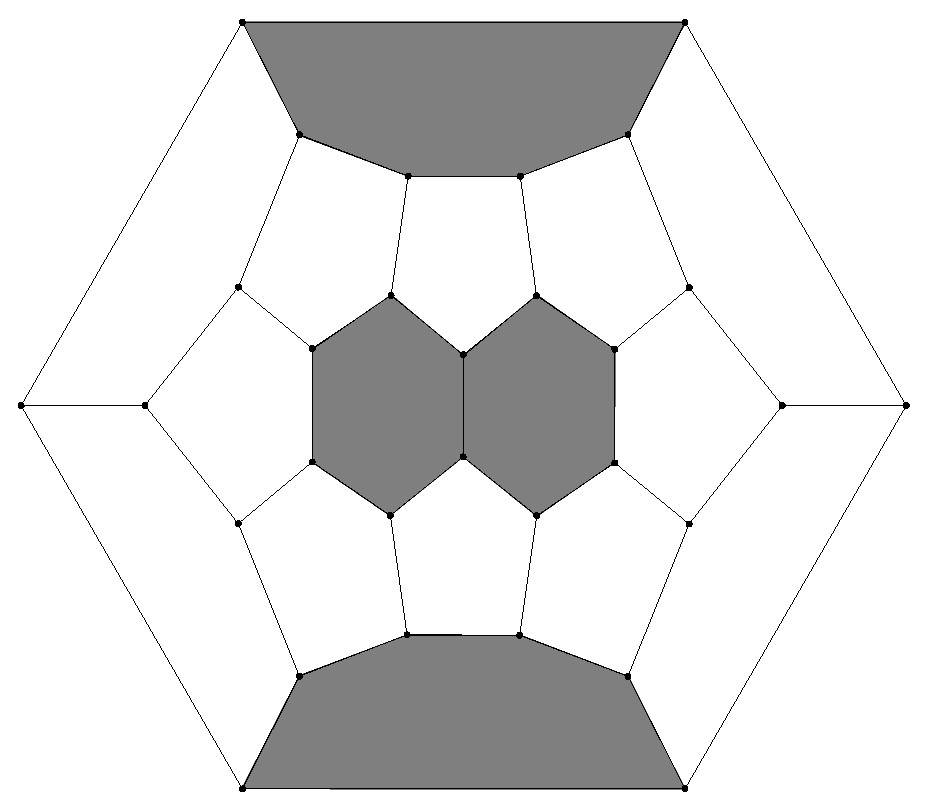
\includegraphics{FullPresPic/Picture6.eps}}\par
30, $C_{2v}$
\end{minipage}
\begin{minipage}[b]{2.7cm}
\centering
\resizebox{25mm}{!}{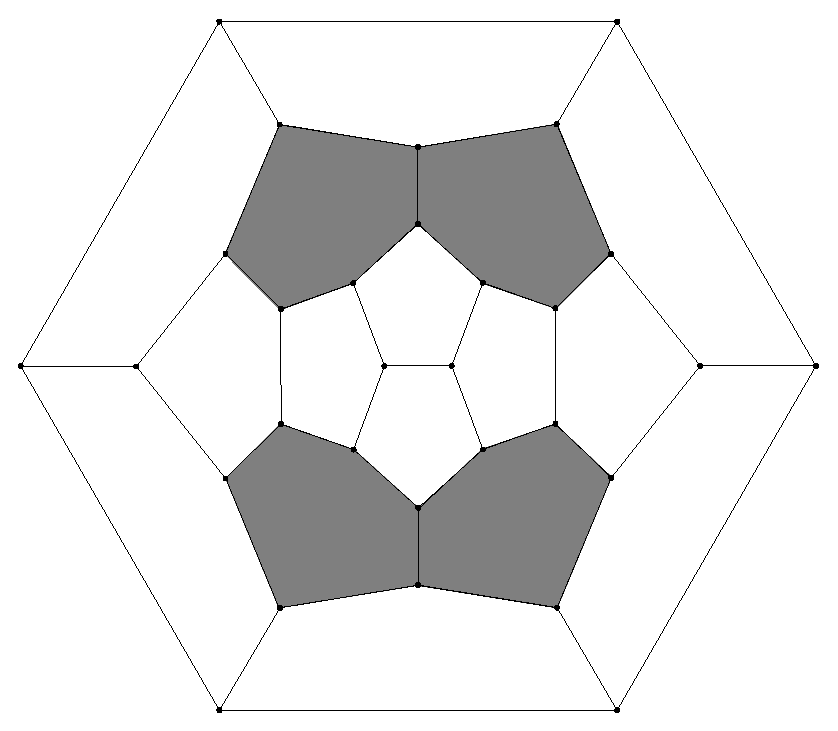
\includegraphics{FullPresPic/Picture7.eps}}\par
30, $D_{2v}$
\end{minipage}
\end{center}
\end{slide}




\begin{slide}{A $C_{540}$}
\begin{center}
\begin{minipage}{8.5cm}
\centering
\resizebox{7.1cm}{!}{\rotatebox{90}{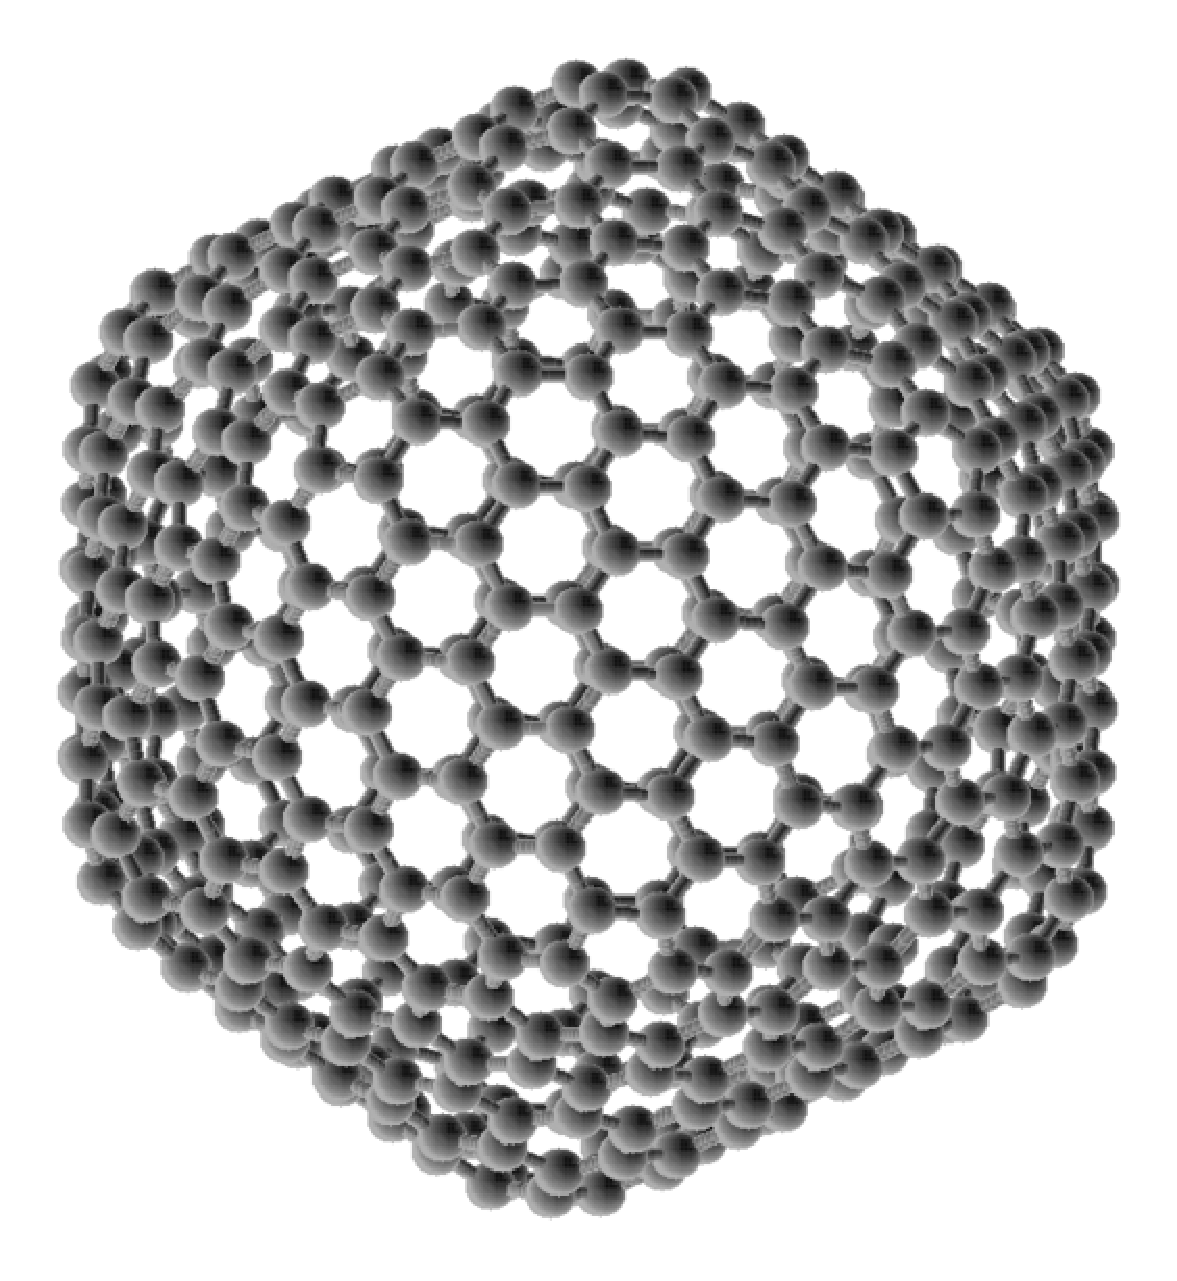
\includegraphics{FullPresPic/Fig.eps}}}\par
\end{minipage}
\end{center}
\end{slide}



\begin{slide}{What nature wants?}
Fullerenes $C_n$ or their duals $C_n^*$ appear in architecture and nanoworld:
\begin{itemize}
\item Biology: virus capsids and clathrine coated vesicles
\item Organic (i.e., carbon) Chemistry
\item also: (energy) minimizers in Thomson problem (for 
$n$ unit charged particles on sphere) and Skyrme problem (for 
given 
baryonic number of nucleons); maximizers, in Tammes problem,
of minimum distance between $n$ points on sphere
\end{itemize}
Simple polyhedra with given number of faces, which are the ``best''
approximation of sphere?


\begin{center}
Conjecture: \textcolor{red}{FULLERENES}
\end{center}
\end{slide}


\begin{slide}{Graver's superfullerenes}

\begin{itemize}
\item Almost all optimizers for Thomson and Tammes problems, in the range
$25 \le n \le 125$ are fullerenes.

\item For $n>125$, appear $7$-gonal faces; almost always for $n>300$.

\item However, J.Graver (2005): in all large optimizers the $5$- and $7$-gonal 
faces occurs in 12 distinct clusters, corresponding to a unique 
underlying fullerene.
\end{itemize}
\end{slide}






\overlays{2}{
\begin{slide}{Isoperimetric problem for polyhedra}
\onlySlide*{1}{
\begin{center}
Lhuilier 1782, Steiner 1842, Lindel\"of 1869, Steinitz 1927, Goldberg 1933, Fejes T\'oth 1948, P\'olya 1954
\end{center}

\begin{itemize}
\item Polyhedron of greatest volume $V$ with a given number of faces and a 
given surface $S$?
\item Polyhedron of least volume with a given number of faces circumscribed 
around a sphere?
\item Maximize \textcolor{red}{Isoperimetric Quotient} for solids $IQ=36\pi
\frac{V^2}{S^3}\leq 1$
 (with equality only for sphere)
\end{itemize}
}
\onlySlide*{2}{
\begin{center}
\begin{tabular}{|c|c|c|}
\hline
polyhedron & $IQ(P)$  & upper bound\\
\hline
Tetrahedron & $\frac{\pi}{6\sqrt{3}}\simeq 0.302$  &$\frac{\pi}{6\sqrt{3}}$\\
Cube        & $\frac{\pi}{6}\simeq 0.524$  &$\frac{\pi}{6}$\\
Octahedron  & $\frac{\pi}{3\sqrt{3}}\simeq 0.605$  &$\simeq 0.637$\\
Dodecahedron& $\frac{\pi \tau^{7/2}}{3.5^{5/4}}\simeq 0.755$ & $\frac{\pi \tau^{7/2}}{3.5^{5/4}}$\\
Icosahedron& $\frac{\pi \tau^{4}}{15\sqrt{3}}\simeq 0.829$ & $\simeq 0.851$\\
\hline
\end{tabular}
\end{center}
\begin{center}
IQ of Platonic solids\\
($\tau=\frac{1+\sqrt{5}}{2}$: {\em golden mean})
\end{center}
{\bf Conjecture} (Steiner 1842):\\
Each of the $5$ Platonic solids is the best of all isomorphic polyhedra (still open for the Icosahedron)
}
\end{slide}
}



\begin{slide}{Five Platonic solids}
\vspace{-5mm}
\begin{center}
\begin{minipage}[t]{3.5cm}
\resizebox{2.8cm}{!}{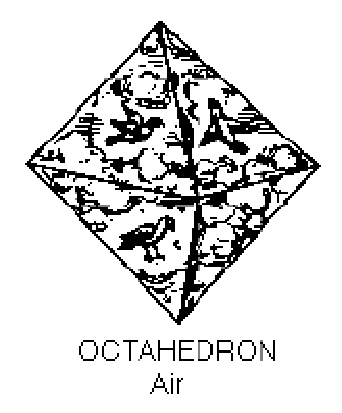
\includegraphics{DRAW/PS/kepler1.ps}}
\end{minipage}
\begin{minipage}[t]{3.5cm}
\resizebox{2.8cm}{!}{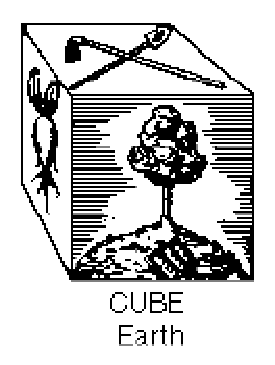
\includegraphics{DRAW/PS/kepler2.ps}}
\end{minipage}
\begin{minipage}[t]{3.5cm}
\resizebox{2.8cm}{!}{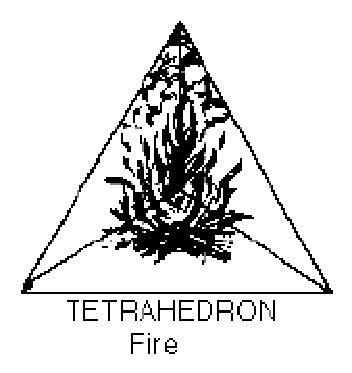
\includegraphics{DRAW/PS/kepler3.ps}}
\end{minipage}
\begin{minipage}[t]{3.5cm}
\resizebox{2.8cm}{!}{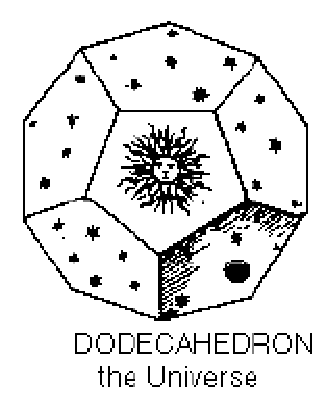
\includegraphics{DRAW/PS/kepler4.ps}}
\end{minipage}
\begin{minipage}[t]{3.5cm}
\resizebox{2.8cm}{!}{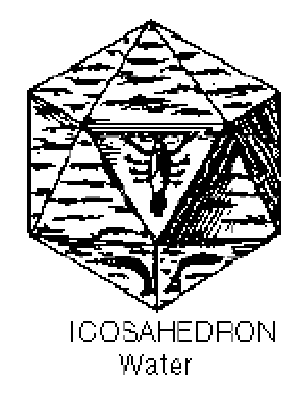
\includegraphics{DRAW/PS/kepler5.ps}}
\end{minipage}
\end{center}

\end{slide}



\begin{slide}{Goldberg Conjecture}
\vspace{-7mm}
\begin{center}
\begin{center}
\resizebox{2.9cm}{!}{\includegraphics{DRAW/PS/F36.ps}}
\end{center}
$IQ(Icosahedron)  \leq IQ(F_{36})\simeq 0.848$
\end{center}

{\bf Conjecture} (Goldberg 1933):\\
The polyhedron with $m\geq 12$ facets with greatest $IQ$ is a fullerene (called ``medial polyhedron'' by Goldberg)

%{\small
\begin{center}
\begin{tabular}{|c|c|c|}
\hline
polyhedron & $IQ(P)$  & upper bound\\
\hline\hline
Dodecahedron $F_{20}(I_h)$& $\frac{\pi \tau^{7/2}}{3.5^{5/4}}\simeq 0.755$ & $\frac{\pi \tau^{7/2}}{3.5^{5/4}}$\\\hline
Truncated icosahedron $C_{60}(I_h)$&$\simeq 0.9058$ & $\simeq 0.9065$\\\hline
Chamfered dodecahed. $C_{80}(I_h)$&$\simeq 0.928$ & $\simeq 0.929$\\\hline
Sphere &$1$ & $1$\\\hline\hline
\end{tabular}
\end{center}
%}

\end{slide}


\begin{slide}{}
\begin{center}
{\Huge 
\begin{tabular*}{7cm}{c}
\\[-0.3cm]
\textcolor{blue}{II. }\textcolor{red}{Icosahedral}\\
\textcolor{red}{fullerenes}
\end{tabular*}
}
\end{center}
\end{slide}


\begin{slide}{Icosahedral fullerenes}
\vspace{-6mm}
Call \textcolor{red}{icosahedral} any fullerene with symmetry $I_h$ or $I$
\begin{itemize}
\item All icosahedral fullerenes are preferable, except $F_{20}(I_h)$
\item $n=20T$, where $T=a^2+ab+b^2$ (\textcolor{blue}{triangulation number})
 with $0\leq b\leq a$.

\item $I_h$ for $a=b\not= 0$ or $b=0$ (extended icosahedral group);\\
$I$ for $0<b<a$ (proper icosahedral group)
\end{itemize}

\begin{center}
\begin{minipage}{5.5cm}
\resizebox{3.5cm}{!}{\includegraphics{DRAW/PS/C60.ps}}\par
$C_{60}(I_h)$=$(1,1)$-dodecahedron\\
truncated icosahedron
\end{minipage}
\begin{minipage}{5.5cm}
\resizebox{3.5cm}{!}{\includegraphics{DRAW/PS/C80.ps}}\par
$C_{80}(I_h)$=$(2,0)$-dodecahedron\\
chamfered dodecahedron
\end{minipage}
\end{center}

\end{slide}




\begin{slide}{Icosadeltahedra}

Call \textcolor{red}{icosadeltahedron} the dual of an icosahedral fullerene $C_{20T}^*(I_h)$ or $C_{20T}^*(I)$
\begin{itemize}
\item Geodesic domes: B.Fuller
\item Capsids of viruses: Caspar and Klug, Nobel prize 1962
\end{itemize}

\begin{center}
\begin{minipage}[b]{5.5cm}
\centering
\resizebox{3.5cm}{!}{\includegraphics{DRAW/PS/embeddingofdualC60.ps}}\par
Dual $C_{60}^{*}(I_h)$, $(a,b)=(1,1)$\\
pentakis-dodecahedron
\end{minipage}
\begin{minipage}[b]{5.5cm}
\centering
\resizebox{3.5cm}{!}{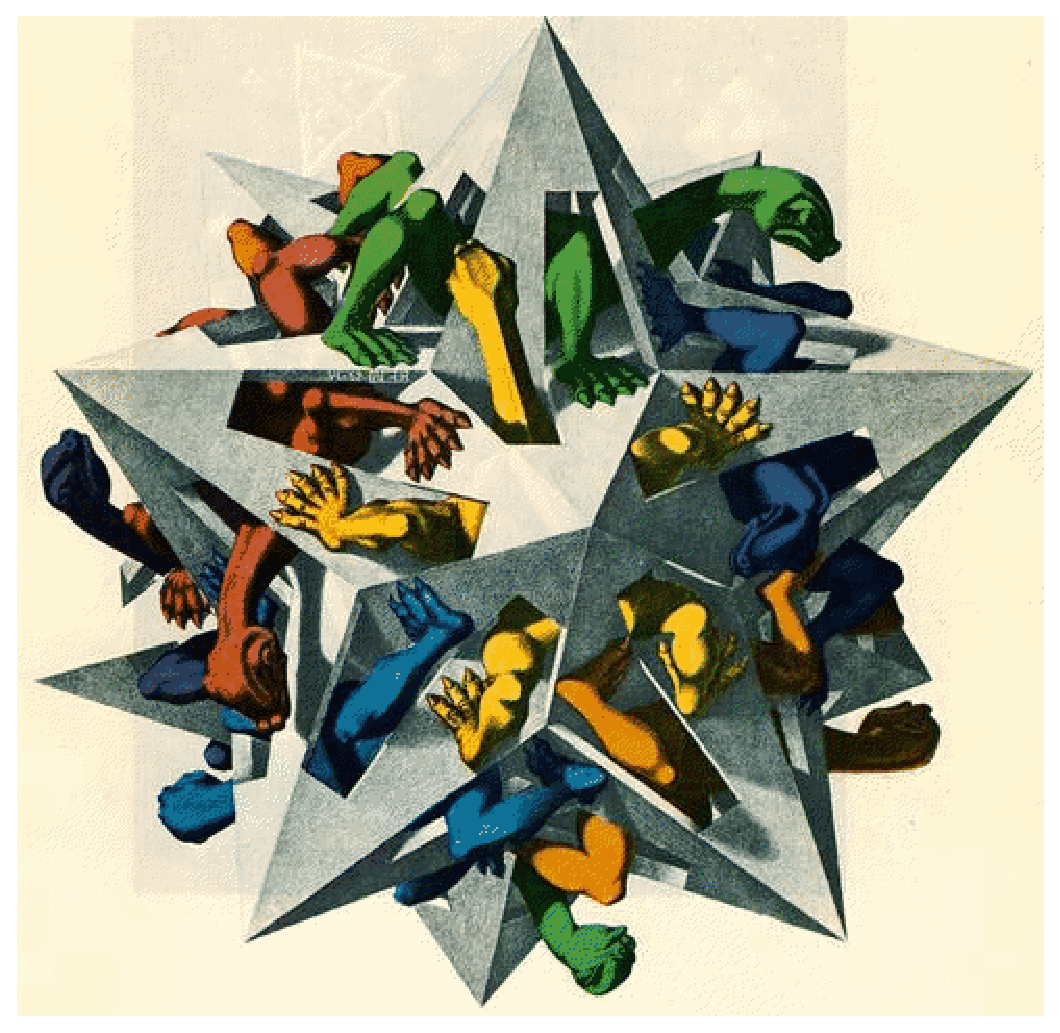
\includegraphics{DRAW/PS/escher.ps}}\par
GRAVIATION (Esher 1952)\\
omnicapped dodecahedron
\end{minipage}
\end{center}


\end{slide}


\begin{slide}{Icosadeltahedra in Architecture}
\begin{center}
{\tiny
\begin{tabular}{|c|c|c|}
\hline
$(a,b)$&Fullerene  & Geodesic dome\\
\hline
$(1,0)$& $F_{20}^*(I_h)$&One of Salvador Dali houses\\
$(1,1)$& $C_{60}^*(I_h)$&Artic Institute, Baffin Island\\
$(3,0)$& $C_{180}^*(I_h)$&Bachelor officers quarters, US Air Force, Korea\\
$(2,2)$& $C_{240}^*(I_h)$&U.S.S. Leyte\\
$(4,0)$& $C_{320}^*(I_h)$&Geodesic Sphere, Mt Washington, New Hampshire\\
$(5,0)$& $C_{500}^*(I_h)$&US pavilion, Kabul Afghanistan\\
$(6,0)$& $C_{720}^*(I_h)$&Radome, Artic dEW\\
$(8,8)$& $C_{3840}^*(I_h)$&Lawrence, Long Island\\
$(16,0)$& $C_{5120}^*(I_h)$&US pavilion, Expo 67, Montreal\\
$(18,0)$& $C_{6480}^*(I_h)$&G\'eode du Mus\'ee des Sciences, La Villete, Paris\\
$(18,0)$& $C_{6480}^*(I_h)$&Union Tank Car, Baton Rouge, Louisiana\\
\hline
\end{tabular}
}
\end{center}
$b=0$ \textcolor{red}{Alternate}, $b=a$ \textcolor{red}{Triacon} and $a+b$ \textcolor{red}{Frequency} (distance of 
two $5$-valent neighbors) are Buckminster Fullers's terms

\end{slide}


\begin{slide}{}
\begin{center}
\begin{minipage}[b]{5.5cm}
\centering
\resizebox{3.5cm}{!}{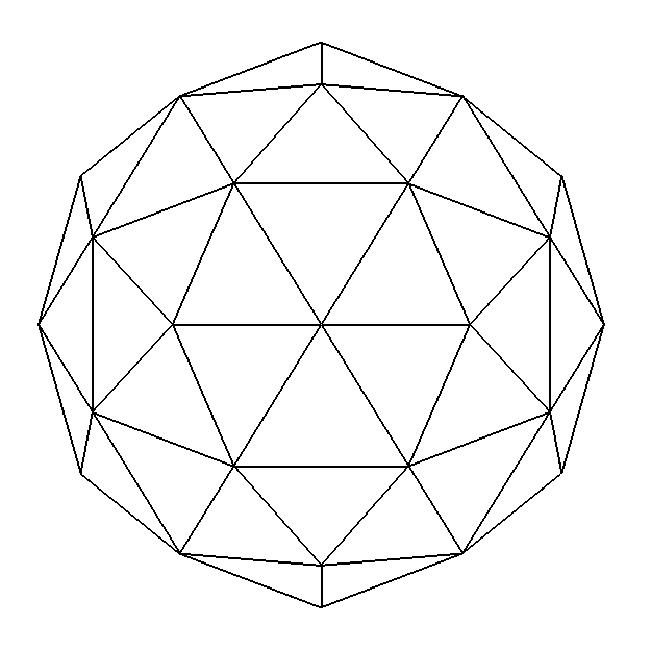
\includegraphics{DRAW/PS/heche2dode.ps}}\par
$C_{80}^*(I_h)$,  $(a,b)$=$(2,0)$
\end{minipage}
\begin{minipage}[b]{5.5cm}
\centering
\resizebox{3.5cm}{!}{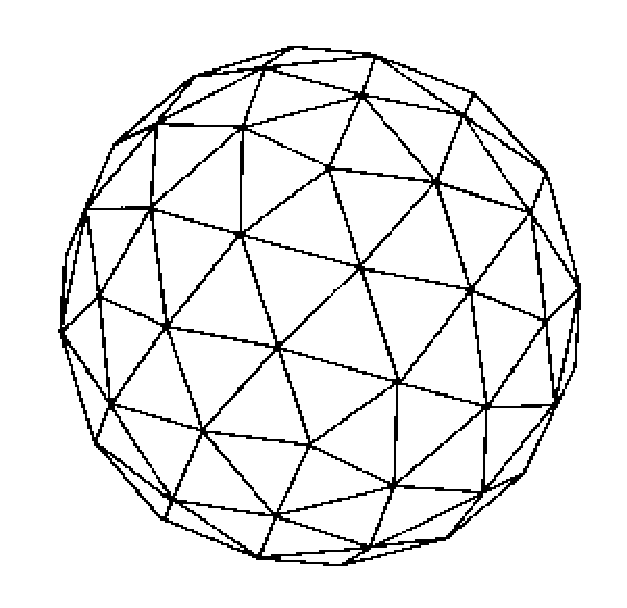
\includegraphics{DRAW/PS/cox140.ps}}\par
$C_{140}^*(I)$,  $(a,b)$=$(2,1)$
\end{minipage}
\end{center}
\end{slide}



\begin{slide}{}
\begin{center}
\begin{minipage}[b]{5.5cm}
\centering
\resizebox{3.5cm}{!}{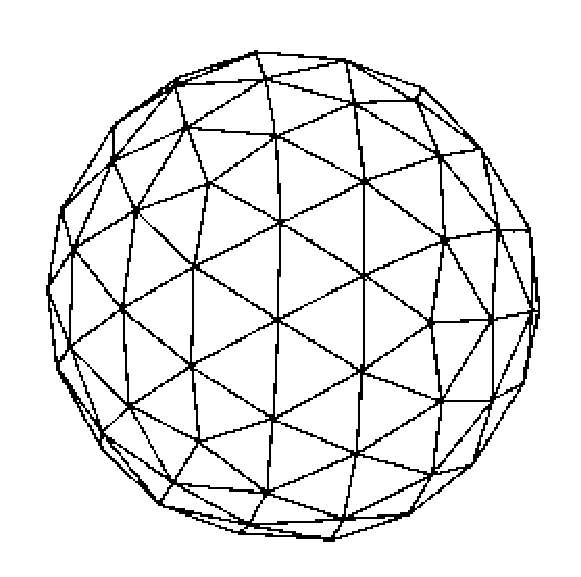
\includegraphics{DRAW/PS/cox180.ps}}\par
$C_{180}^*(I_h)$, $(a,b)=(3,0)$\\
\textcolor{white}{Bonjour}
%Icosadeltahedron $C_{180}^*(I_h)$\\
%Bachelor officers quarters, US Air Force, Korea
\end{minipage}
\begin{minipage}[b]{5.5cm}
\centering
\resizebox{3.5cm}{!}{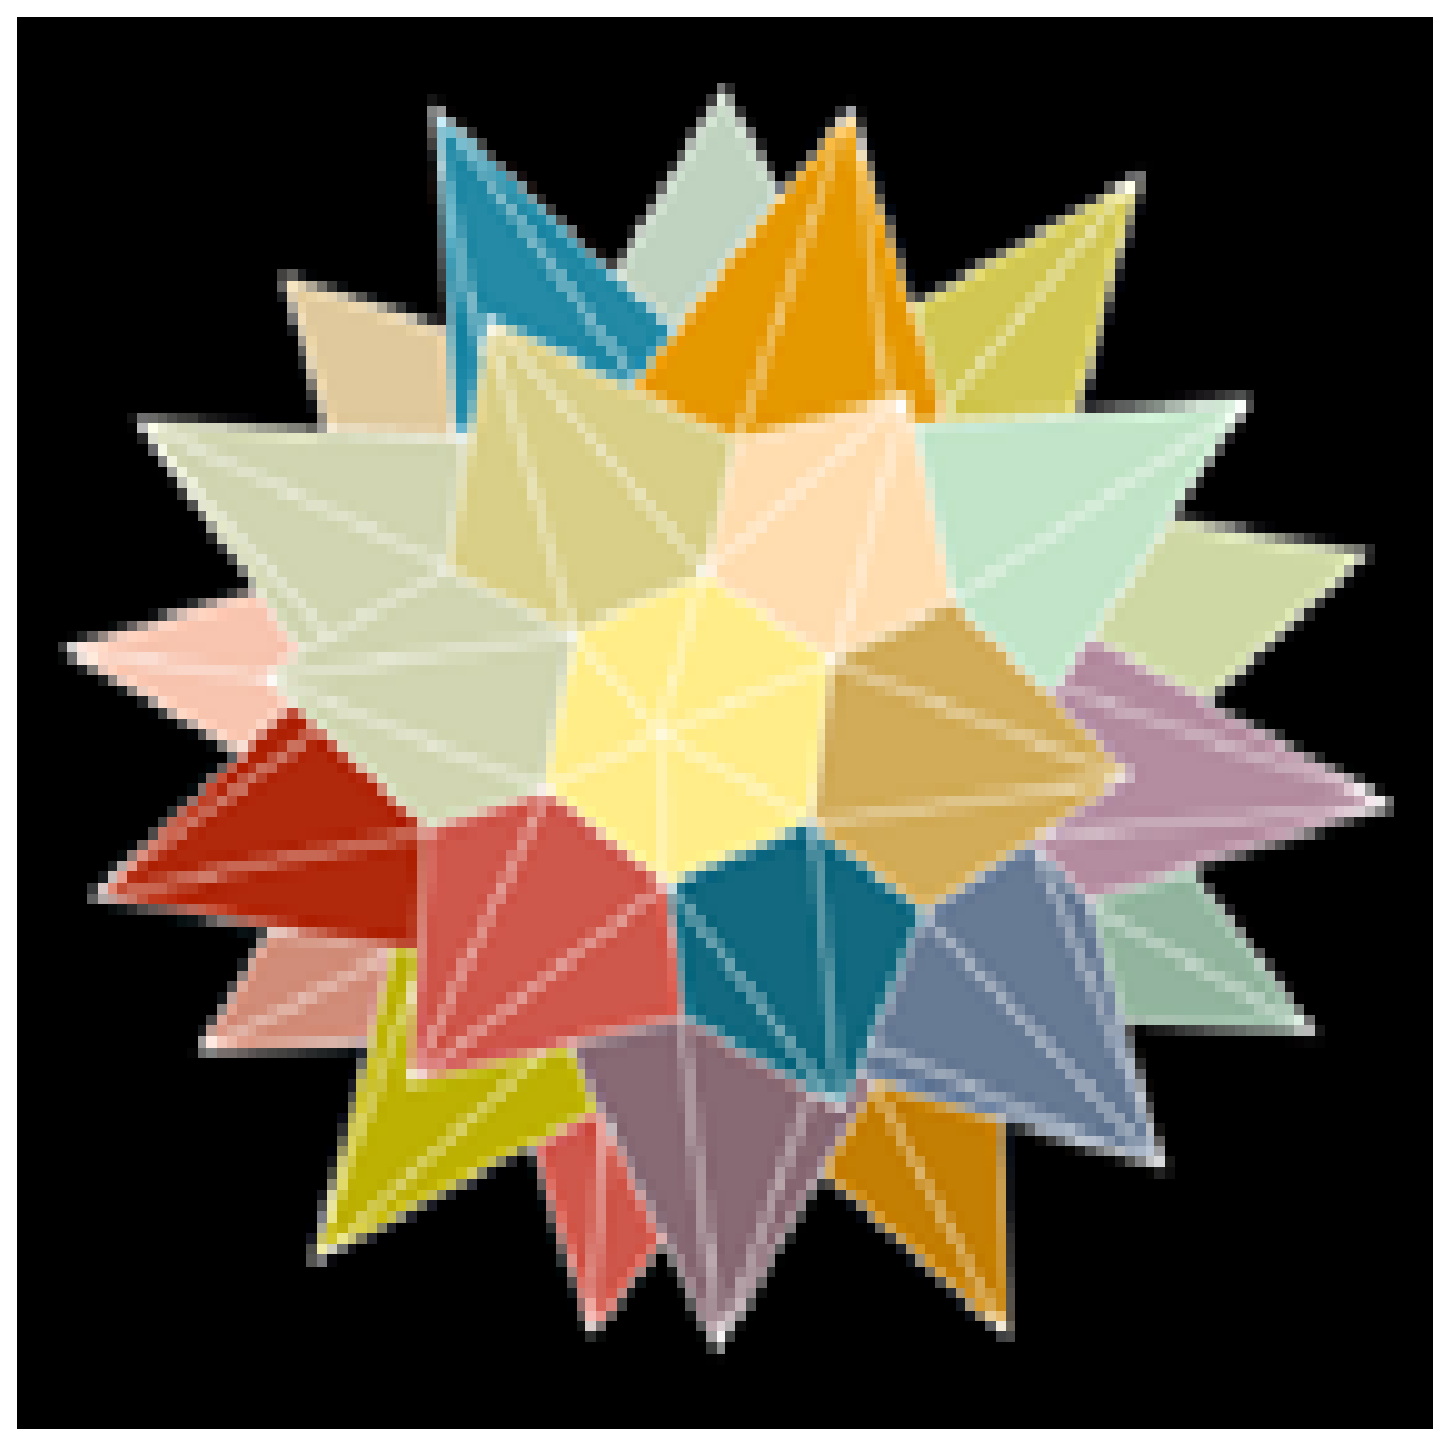
\includegraphics{DRAW/PS/etoile1.ps}}\par
$C_{180}^*(I_h)$ as omnicapped buckminsterfullerene $C_{60}$
\end{minipage}
\end{center}
\end{slide}





\begin{slide}{Triangulations, spherical wavelets}
\begin{center}
\begin{minipage}[b]{5.5cm}
\centering
\resizebox{3.5cm}{!}{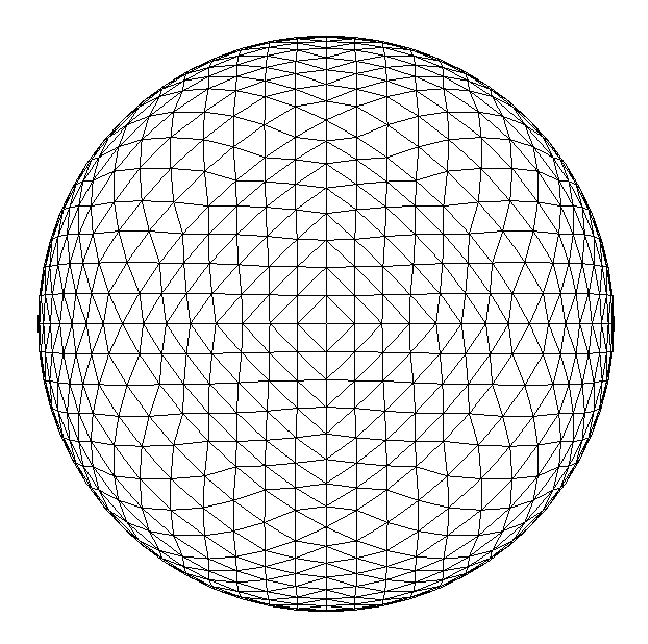
\includegraphics{DRAW/PS/heche4octa.ps}}\par
Dual $4$-chamfered cube \par
$(a,b)=(16,0)$, $O_h$
\end{minipage}
\begin{minipage}[b]{5.5cm}
\centering
\resizebox{3.5cm}{!}{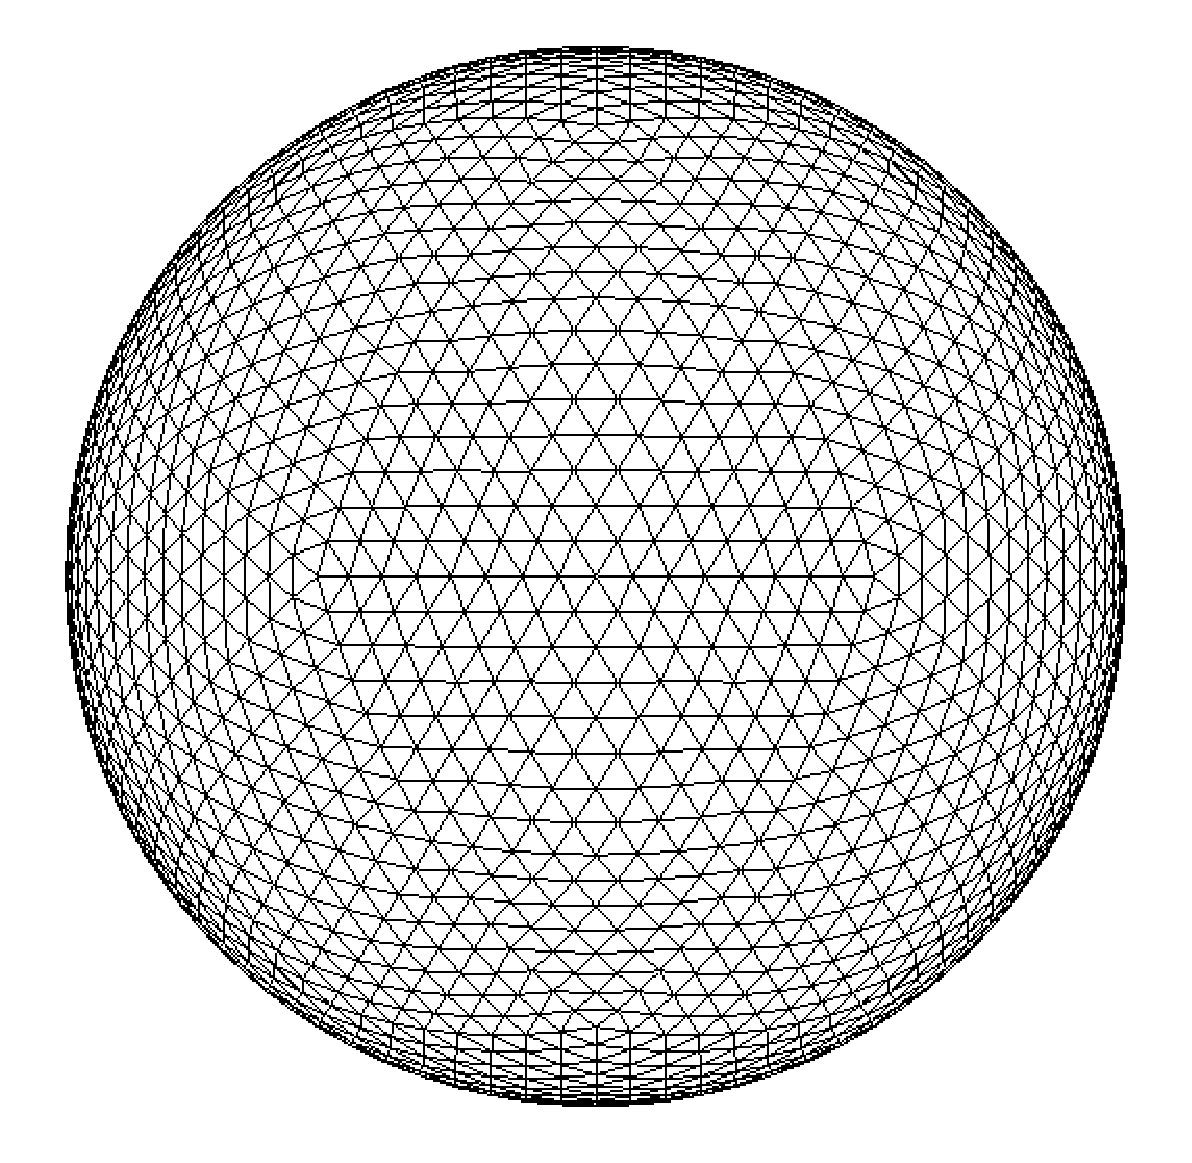
\includegraphics{DRAW/PS/heche4dode.ps}}\par
Dual $4$-cham.
dodecahedron $C^*_{5120}$,
$(a,b)=(16,0)$, $I_h$
%^*(I_h)$ (US pavilion, Expo 67, Montreal)
\end{minipage}
\end{center}
\vspace{7mm}
\begin{center}
Used in Computer Graphics and Topography of Earth
\end{center}



\end{slide}



\begin{slide}{}
\begin{center}
{\Huge 
\begin{tabular*}{8.9cm}{c}
\\[-0.6cm]
\textcolor{blue}{III. }\textcolor{red}{Fullerenes in}\\
\textcolor{red}{Chemistry and Biology}
\end{tabular*}
}
\end{center}
\end{slide}




\begin{slide}{Fullerenes in Chemistry}
Carbon $C$ and, possibly, silicium $Si$ are only $4$-valent elements
producing homoatomic long stable chains or nets
\begin{itemize}
\item \textcolor{red}{Graphite sheet}: bi-lattice $(6^3)$, 
Voronoi partition of the hexagonal lattice ($A_2$), 
``infinite fullerene''
\item \textcolor{red}{Diamond packing}: bi-lattice $D$-complex, 
$\alpha_3$-centering of the lattice f.c.c.=$A_3$
\item \textcolor{red}{Fullerenes}: 1985 (Kroto, Curl, Smalley): 
$C_{60}(I_h)$\\
tr. icosahedon, soccerball, Cayley $A_5$; Nobel prize 1996.\\
But Ozawa (in japanese): 1984. ``Cheap'' $C_{60}$: 1990.\\
1991 (Iijima): \textcolor{red}{nanotubes} (coaxial cylinders).\\
Also isolated chemically by now: $C_{70}$, $C_{76}$, $C_{78}$, 
$C_{82}$, $C_{84}$.\\
If $>100$ carbon atoms, they go on concentric layers; if $<20$, cage opens 
for high $t^{0}$.\\
Full. alloys, stereo org. chemistry, carbon: semi-metal
\end{itemize}

\end{slide}


\overlays{2}{
\begin{slide}{Allotropes of carbon}
\onlySlide*{1}{
\begin{itemize}
\item \textcolor{blue}{Diamond}: cryst.tetrahedral, electro-isolating, hard, transparent.
Rarely $>50$ carats, unique $>800ct$: Cullinan $3106ct=621g$. M.Kuchner: diamond planets?
\item \textcolor{blue}{Graphite}: cryst.hexagonal, soft, opaque, el. conducting
\item \textcolor{blue}{Fullerenes}: 1985, spherical
\item \textcolor{blue}{Nanotubes}: 1991, cylindrical
\item \textcolor{blue}{Carbon nanofoam}: 1997, clusters of about $4000$ atoms linked in graphite-like sheets with some $7$-gons (negatively curved), ferromagnetic
\item \textcolor{blue}{Amorphous carbon} (no long-range pattern): 
synthetic; coal and soot are almost such
\item \textcolor{blue}{White graphite} (chaoite): cryst.hexagonal;
1968, in shock-fused graphite from Ries crater, Bavaria
\end{itemize}
}
\onlySlide*{2}{
\begin{itemize}
\item \textcolor{blue}{Carbon(VI)}: cr.hex.??; 1972, obtained with chaoite
\item \textcolor{blue}{Supersized carbon}: 2005, 5-6 nm supermolecules (benzene rings "atoms", carbon chains "bonds")
\item \textcolor{blue}{Hexagonal diamond} (lonsdaleite):
cryst.hex., very rare; 1967, in  shock-fused graphite from
several meteorites
\item \textcolor{blue}{ANDR} (aggregated diamond nanorods): 2005,
Bayreuth University; hardest known substance
\end{itemize}
\begin{center}
\begin{minipage}[b]{5.5cm}
\centering
graphite: \resizebox{2.7cm}{!}{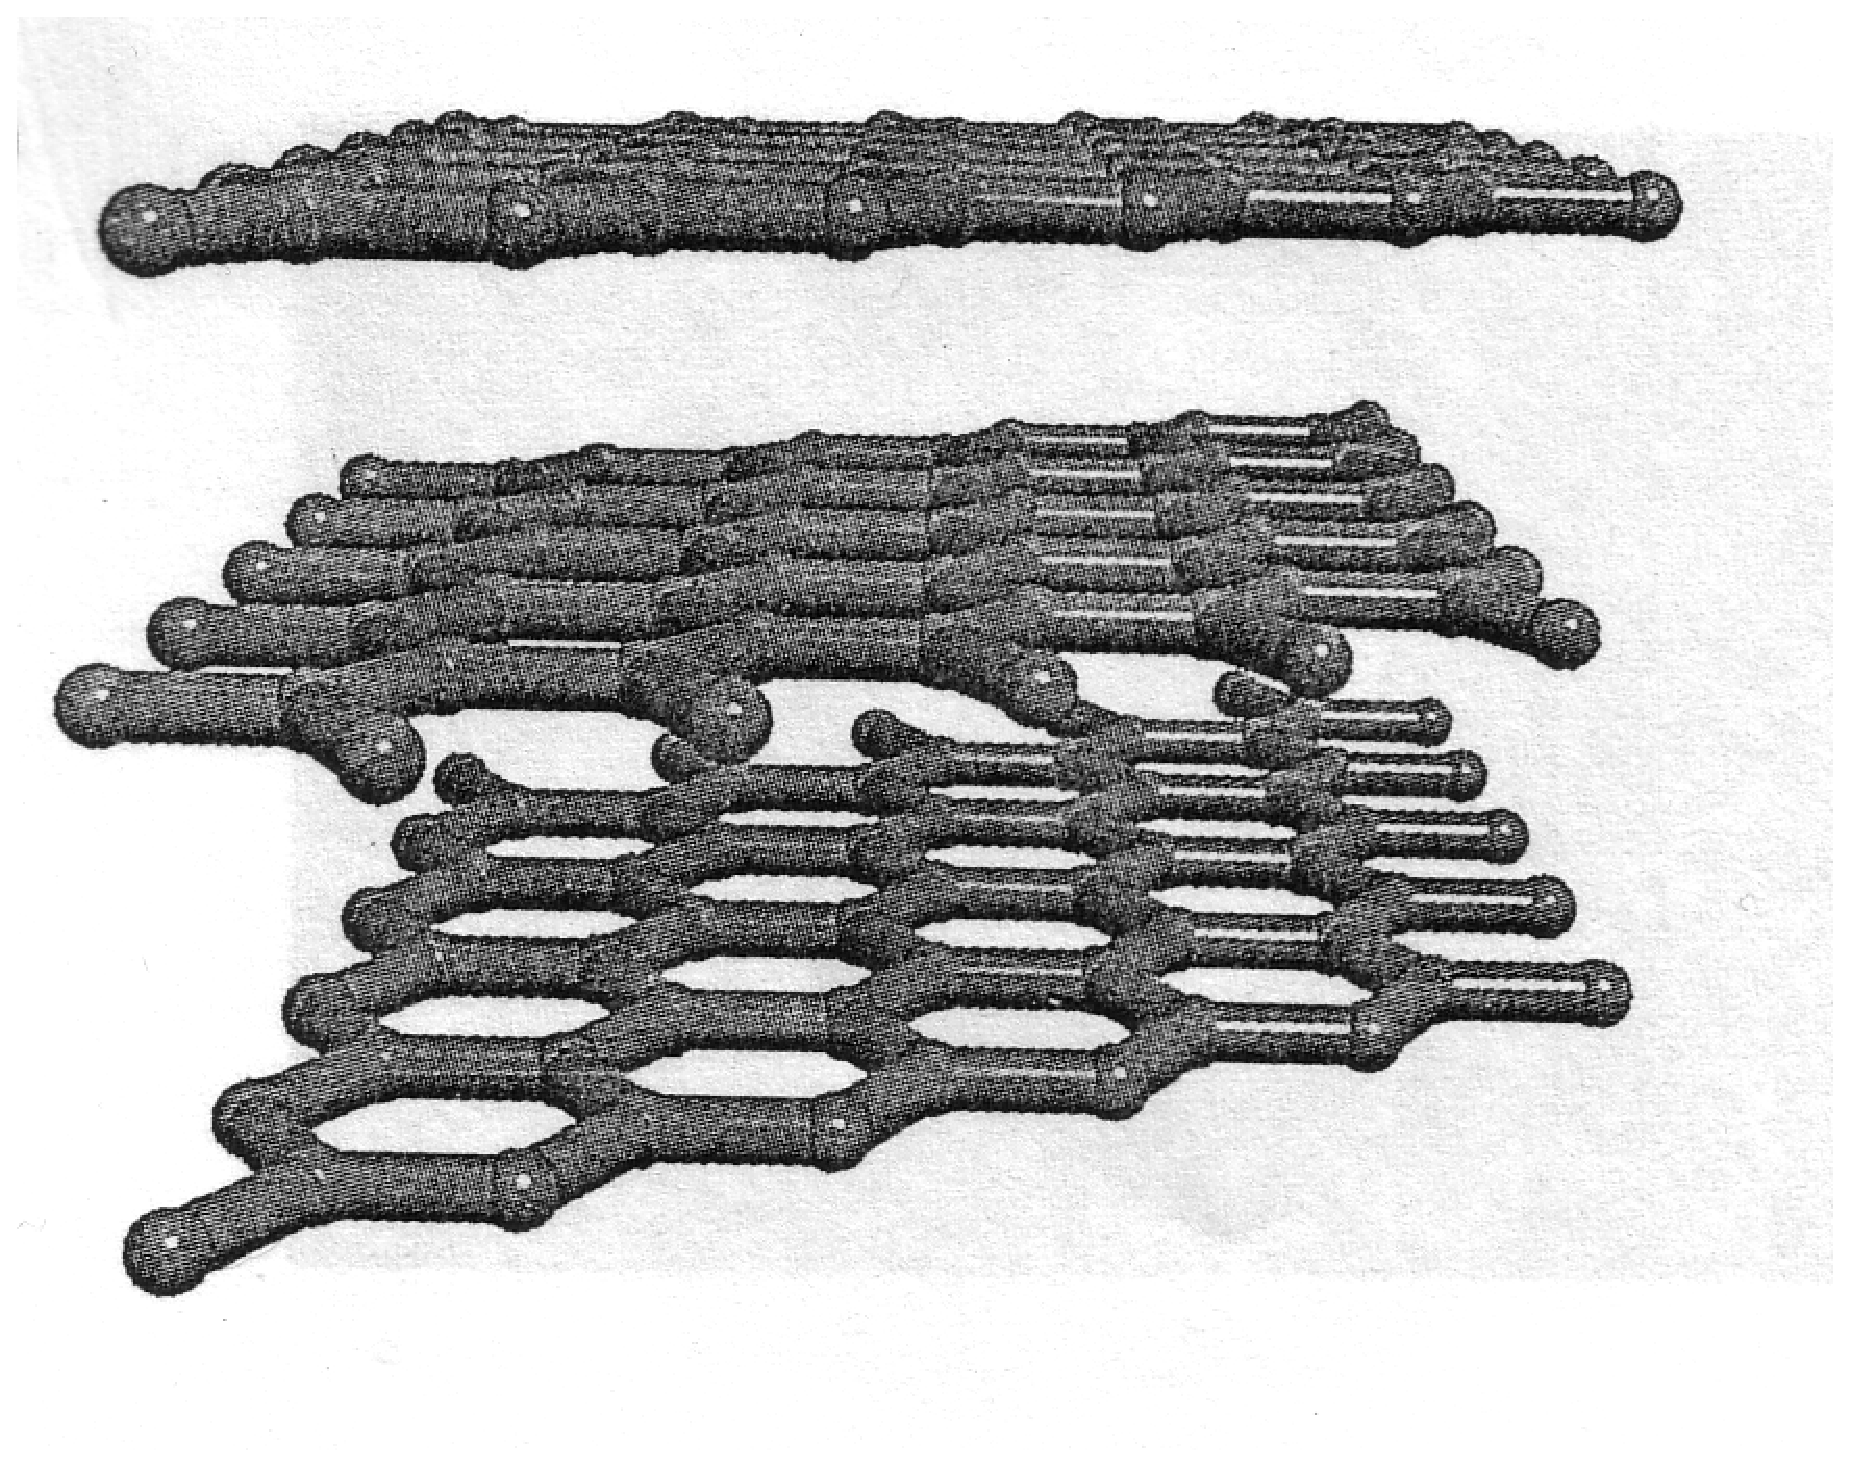
\includegraphics{DRAW/PaperTerrones/P342_1_a.eps}}
\end{minipage}
\begin{minipage}[b]{5.5cm}
\centering
diamond: \resizebox{2.7cm}{!}{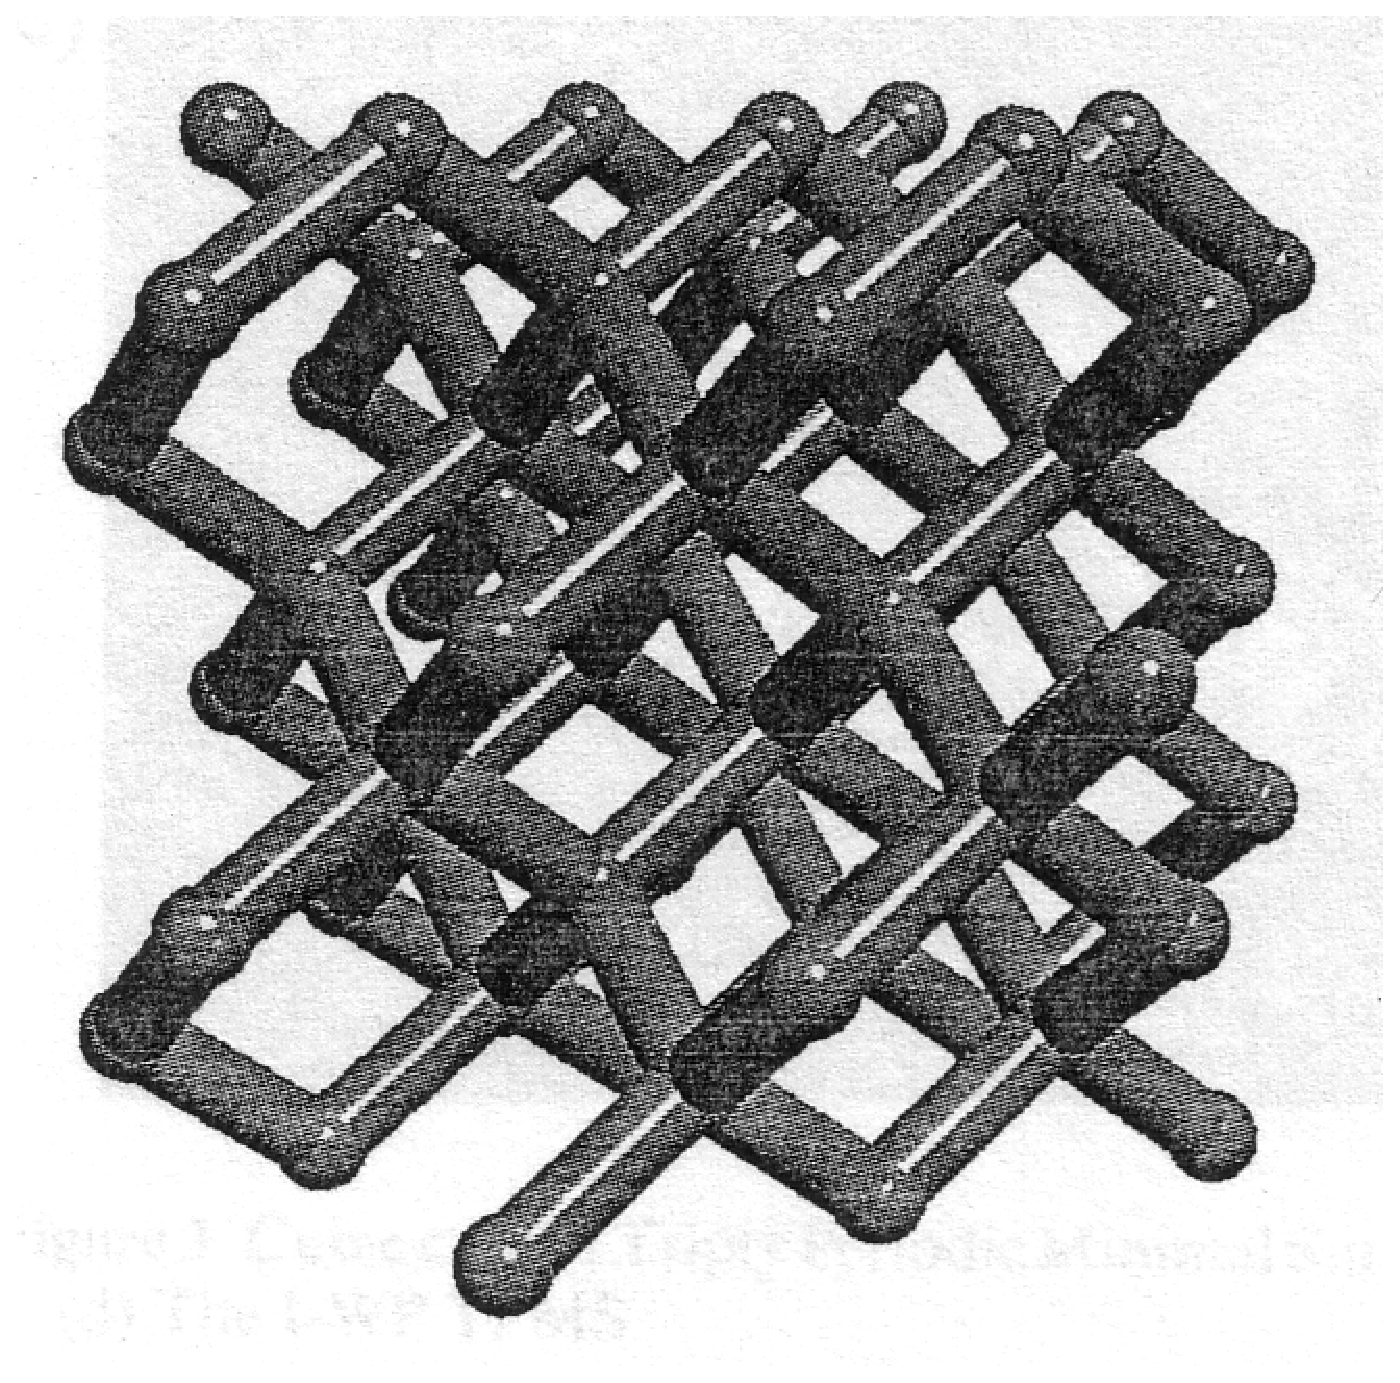
\includegraphics{DRAW/PaperTerrones/P342_1_b.eps}}
\end{minipage}
\end{center}
}
\end{slide}
}




\begin{slide}{}

\begin{center}
\begin{minipage}[b]{5.5cm}
\centering
\resizebox{5.1cm}{!}{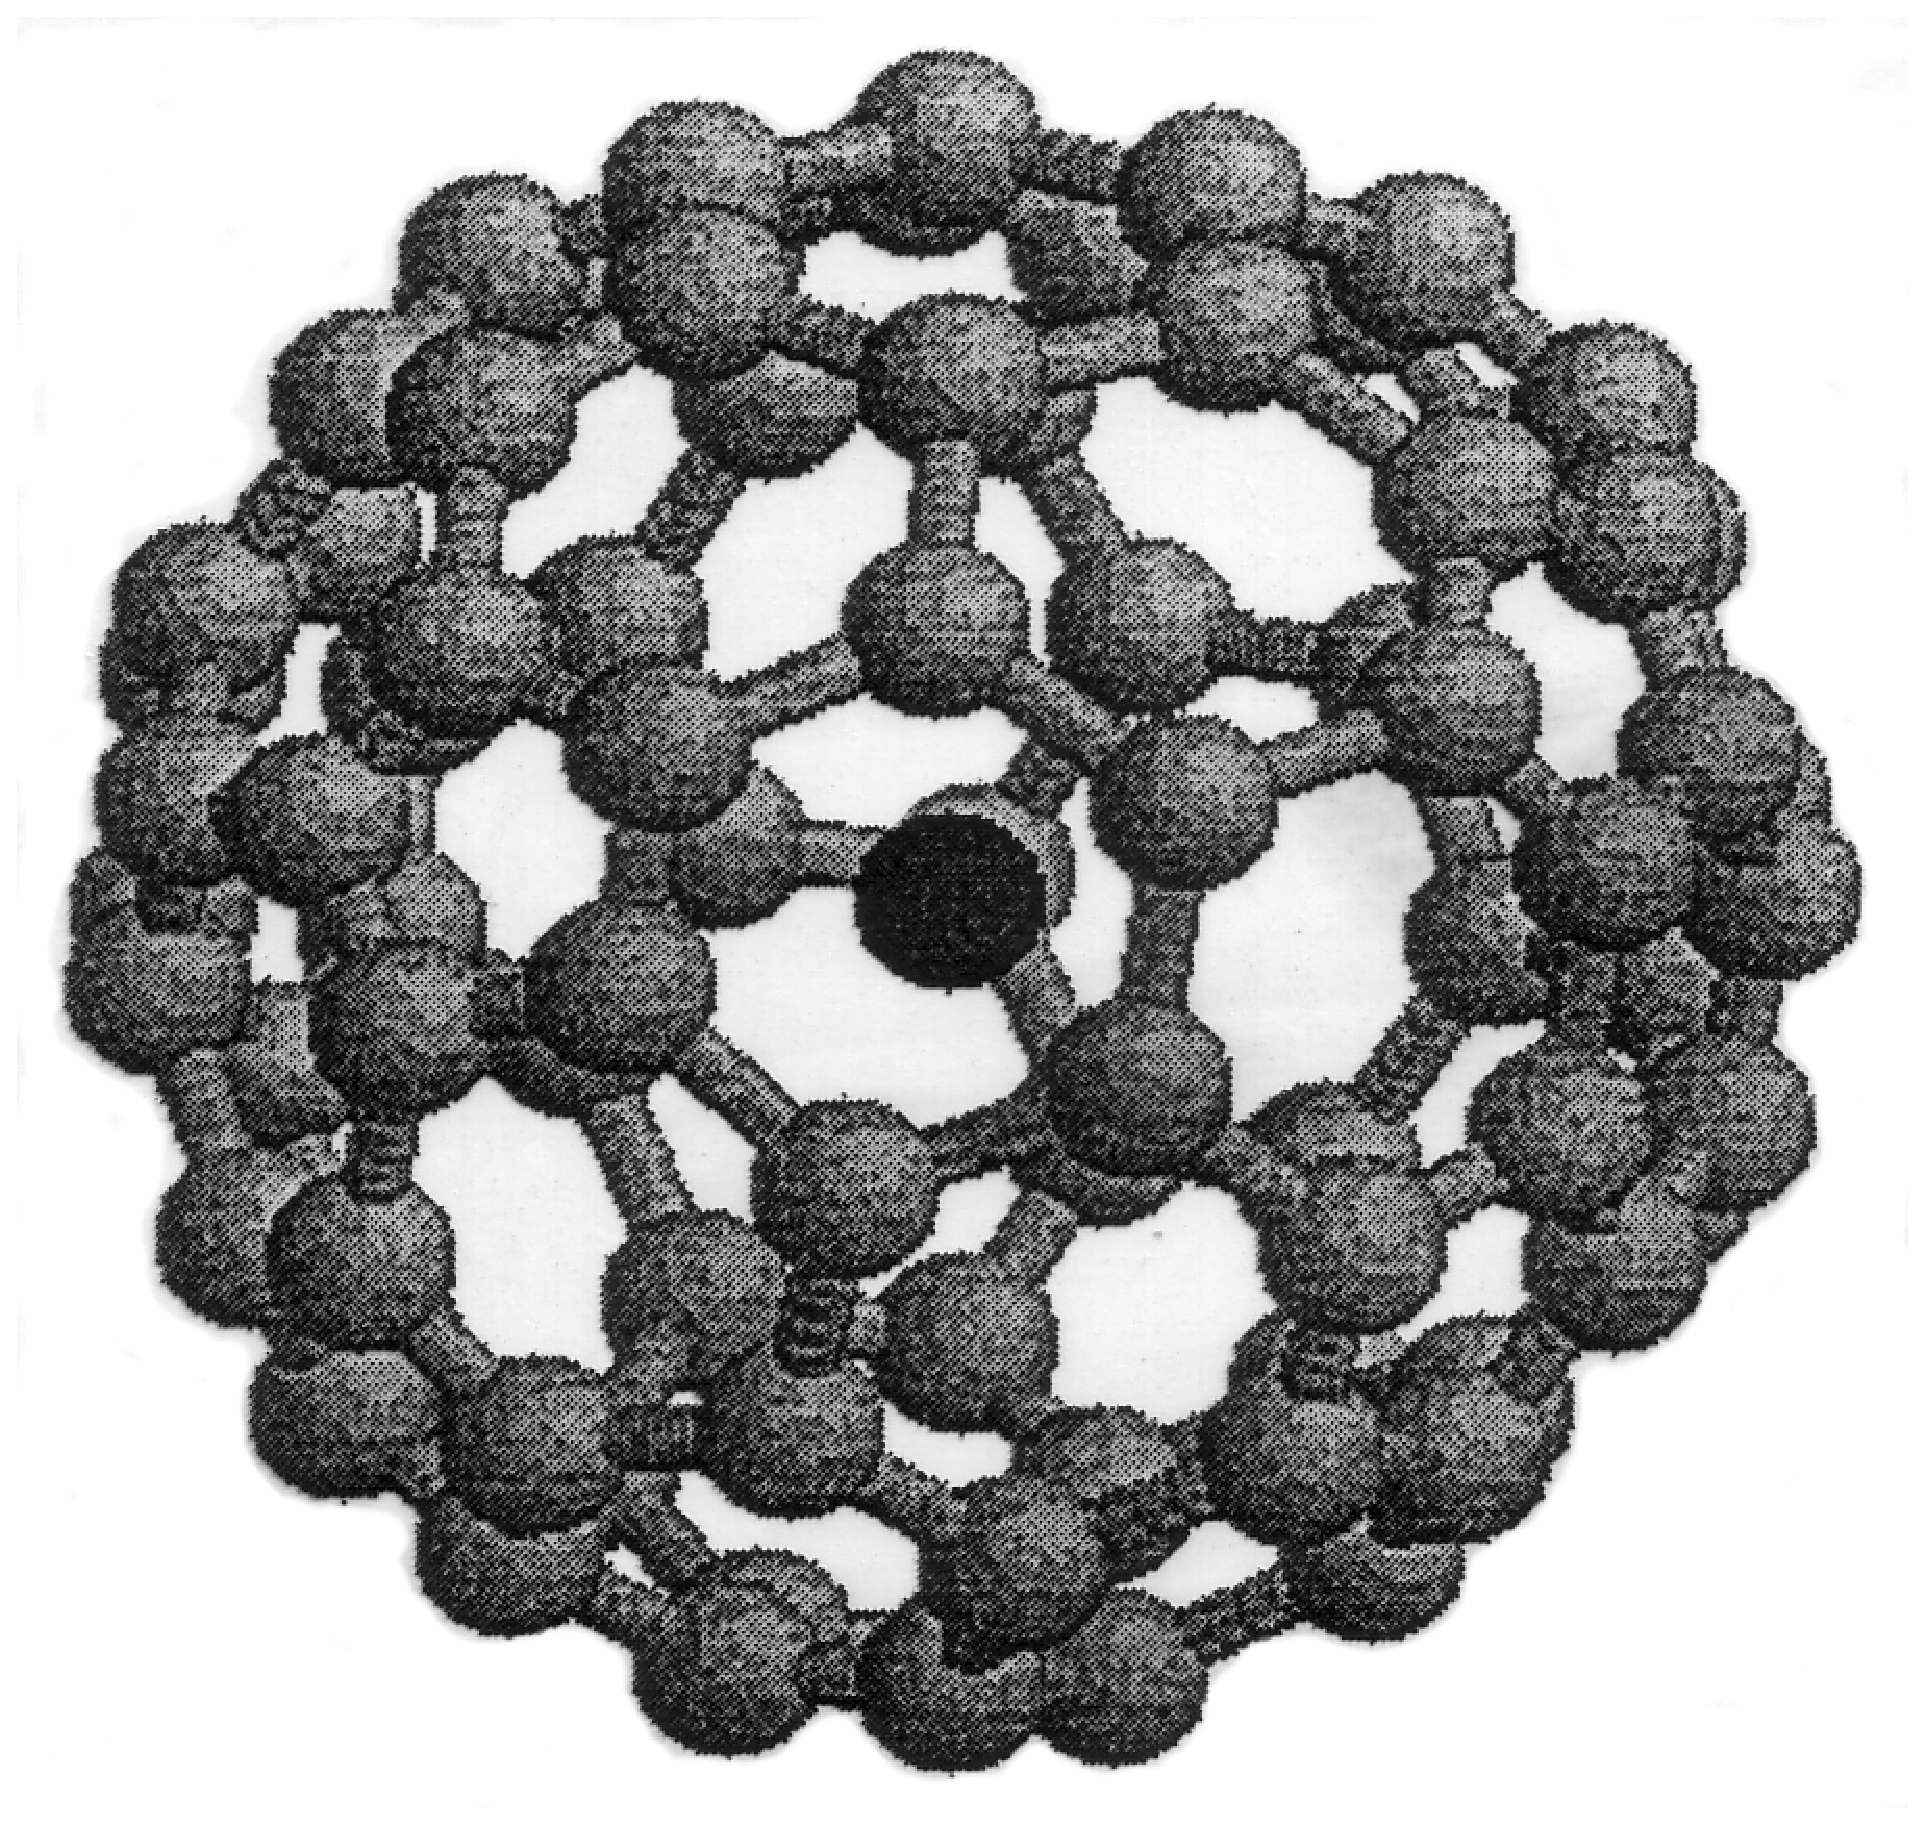
\includegraphics{DRAW/ScanDezaPres/pic3.eps}}\par
La\@$C_{82}$\\
first Endohedral Fullerene compound
\end{minipage}
\begin{minipage}[b]{5.5cm}
\centering
\resizebox{5.1cm}{!}{\includegraphics{DRAW/ScanDezaPres/pic4.eps}}\par
$C_{10}Ph_{9}OH$\\
Exohedral Fullerene compound
(first with a single hydroxy group attached)
\end{minipage}
\end{center}

\end{slide}


\begin{slide}{A quasicrystalline cluster (H. Terrones)}
\vspace{-4mm}
\begin{center}
\begin{minipage}{8.5cm}
\centering
\resizebox{7.1cm}{!}{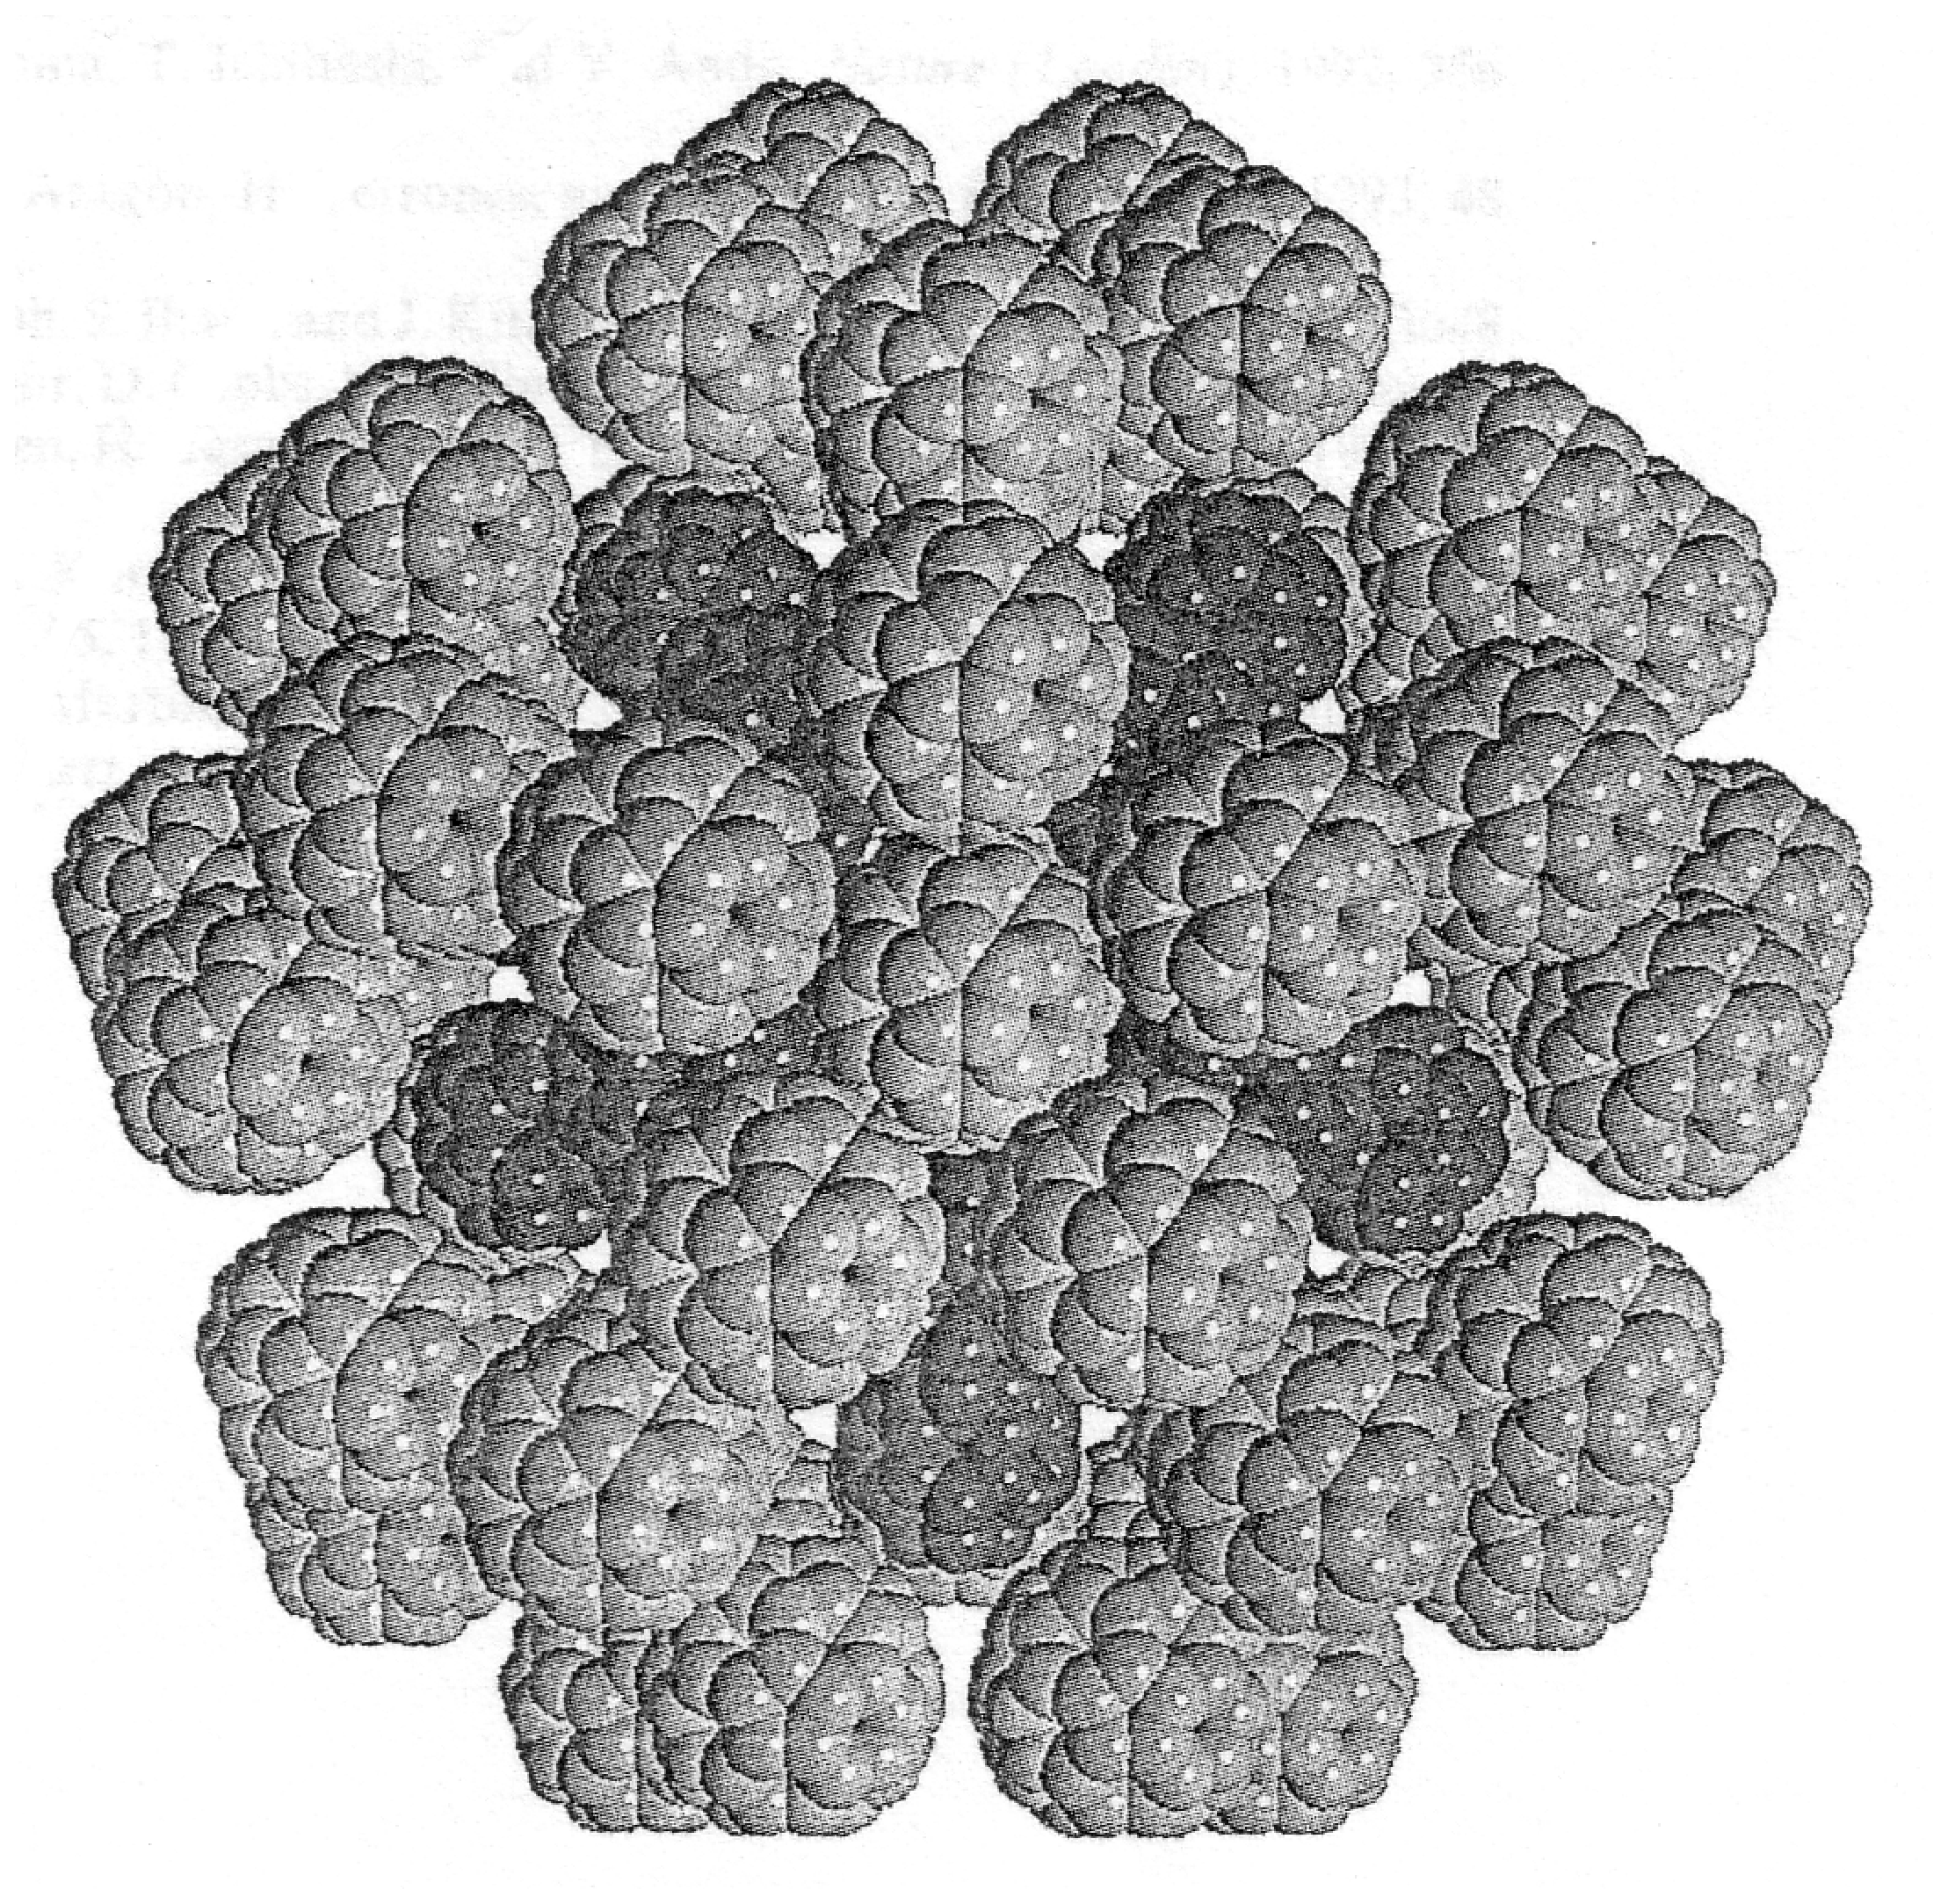
\includegraphics{DRAW/PaperTerrones/P349_13.eps}}\par
\end{minipage}
\end{center}

\begin{center}
In silico: from $C_{60}$ and $F_{40}(T_d)$(dark); cf. 2 atoms in quasicrystals
\end{center}

\end{slide}





\begin{slide}{Onion-like metallic clusters}
\vspace{-0.7cm}
\begin{center}
\begin{minipage}{8.5cm}
\centering
\resizebox{3.5cm}{!}{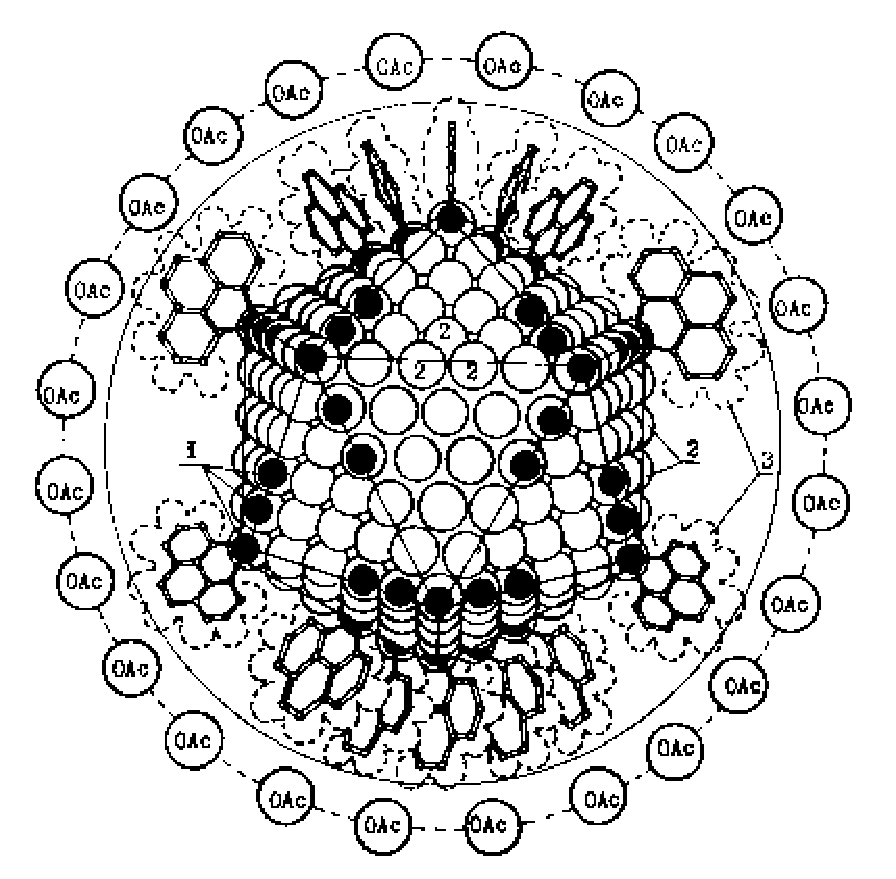
\includegraphics{DRAW/PS/russia.ps}}\par
Palladium icosahedral $5$-cluster $Pd_{561}L_{60}(O_2)_{180}(OAc)_{180}$
\end{minipage}
\end{center}

{\scriptsize
\begin{center}
\begin{tabular}{|c|c|c|c|}
\hline
$\alpha$   & Outer shell   &  Total \# of atoms   & \# Metallic cluster\\
\hline
$1$    &  $C_{20}^*(I_h)$    & $13$     &  $[Au_{13}(PMe_2Ph)_{10}Cl_2]^{3+}$\\
$2$    &  $RhomDode_{80}^{*}(O_h)$  & $55$  &$Au_{55}(PPh_3)_{12}  Cl_{6}$\\
$4$    &   $RhomDode_{320}^{*}(O_h)$ & $309$  &$Pt_{309}(Phen_{36}O_{30\pm 10})$\\
$5$    &  $C_{500}^*(I_h)$    & $561$ &  $Pd_{561}L_{60}(O_2)_{180}(OAc)_{180}$\\
\hline
\end{tabular}
\end{center}
\begin{center}
Icosahedral and cuboctahedral metallic clusters
\end{center}
}

\end{slide}







\begin{slide}{Nanotubes and Nanotechnology}
\vspace{-0.6cm}
\begin{center}
\begin{minipage}[b]{5.5cm}
\centering
\resizebox{4.9cm}{!}{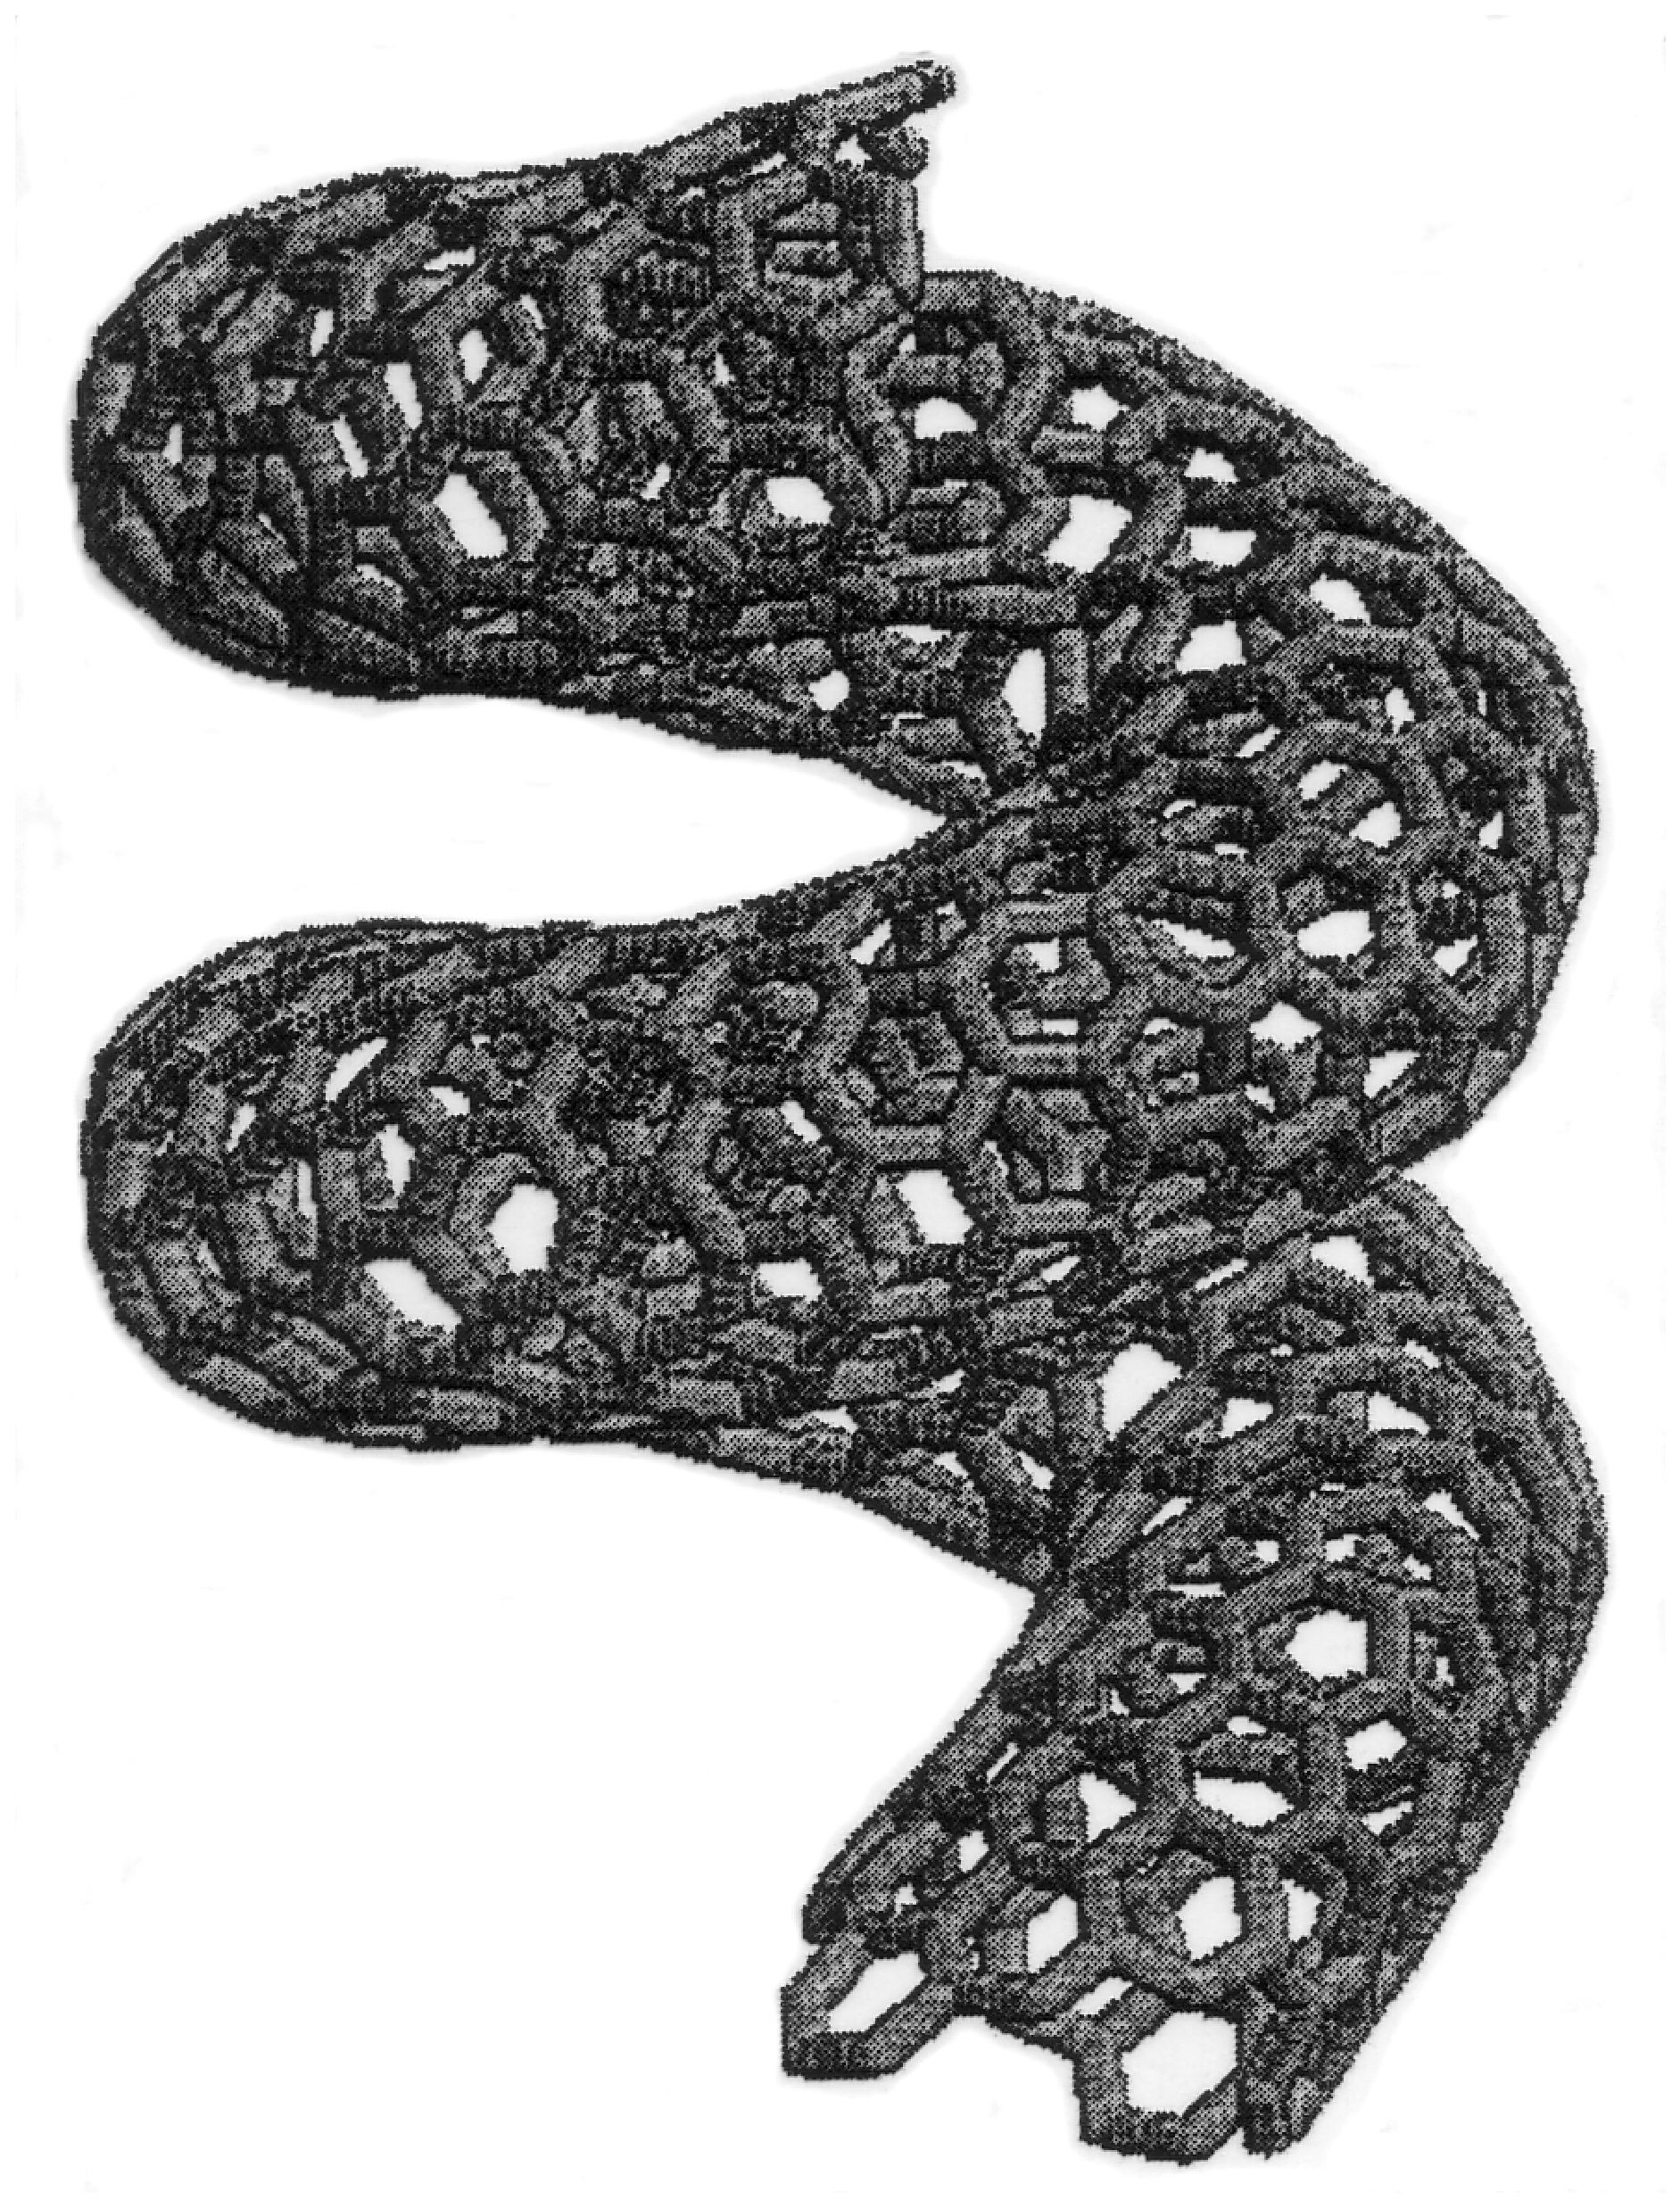
\includegraphics{DRAW/ScanDezaPres/pic1.eps}}\par
Helical graphite
\end{minipage}
\begin{minipage}[b]{5.5cm}
\centering
\resizebox{4.1cm}{!}{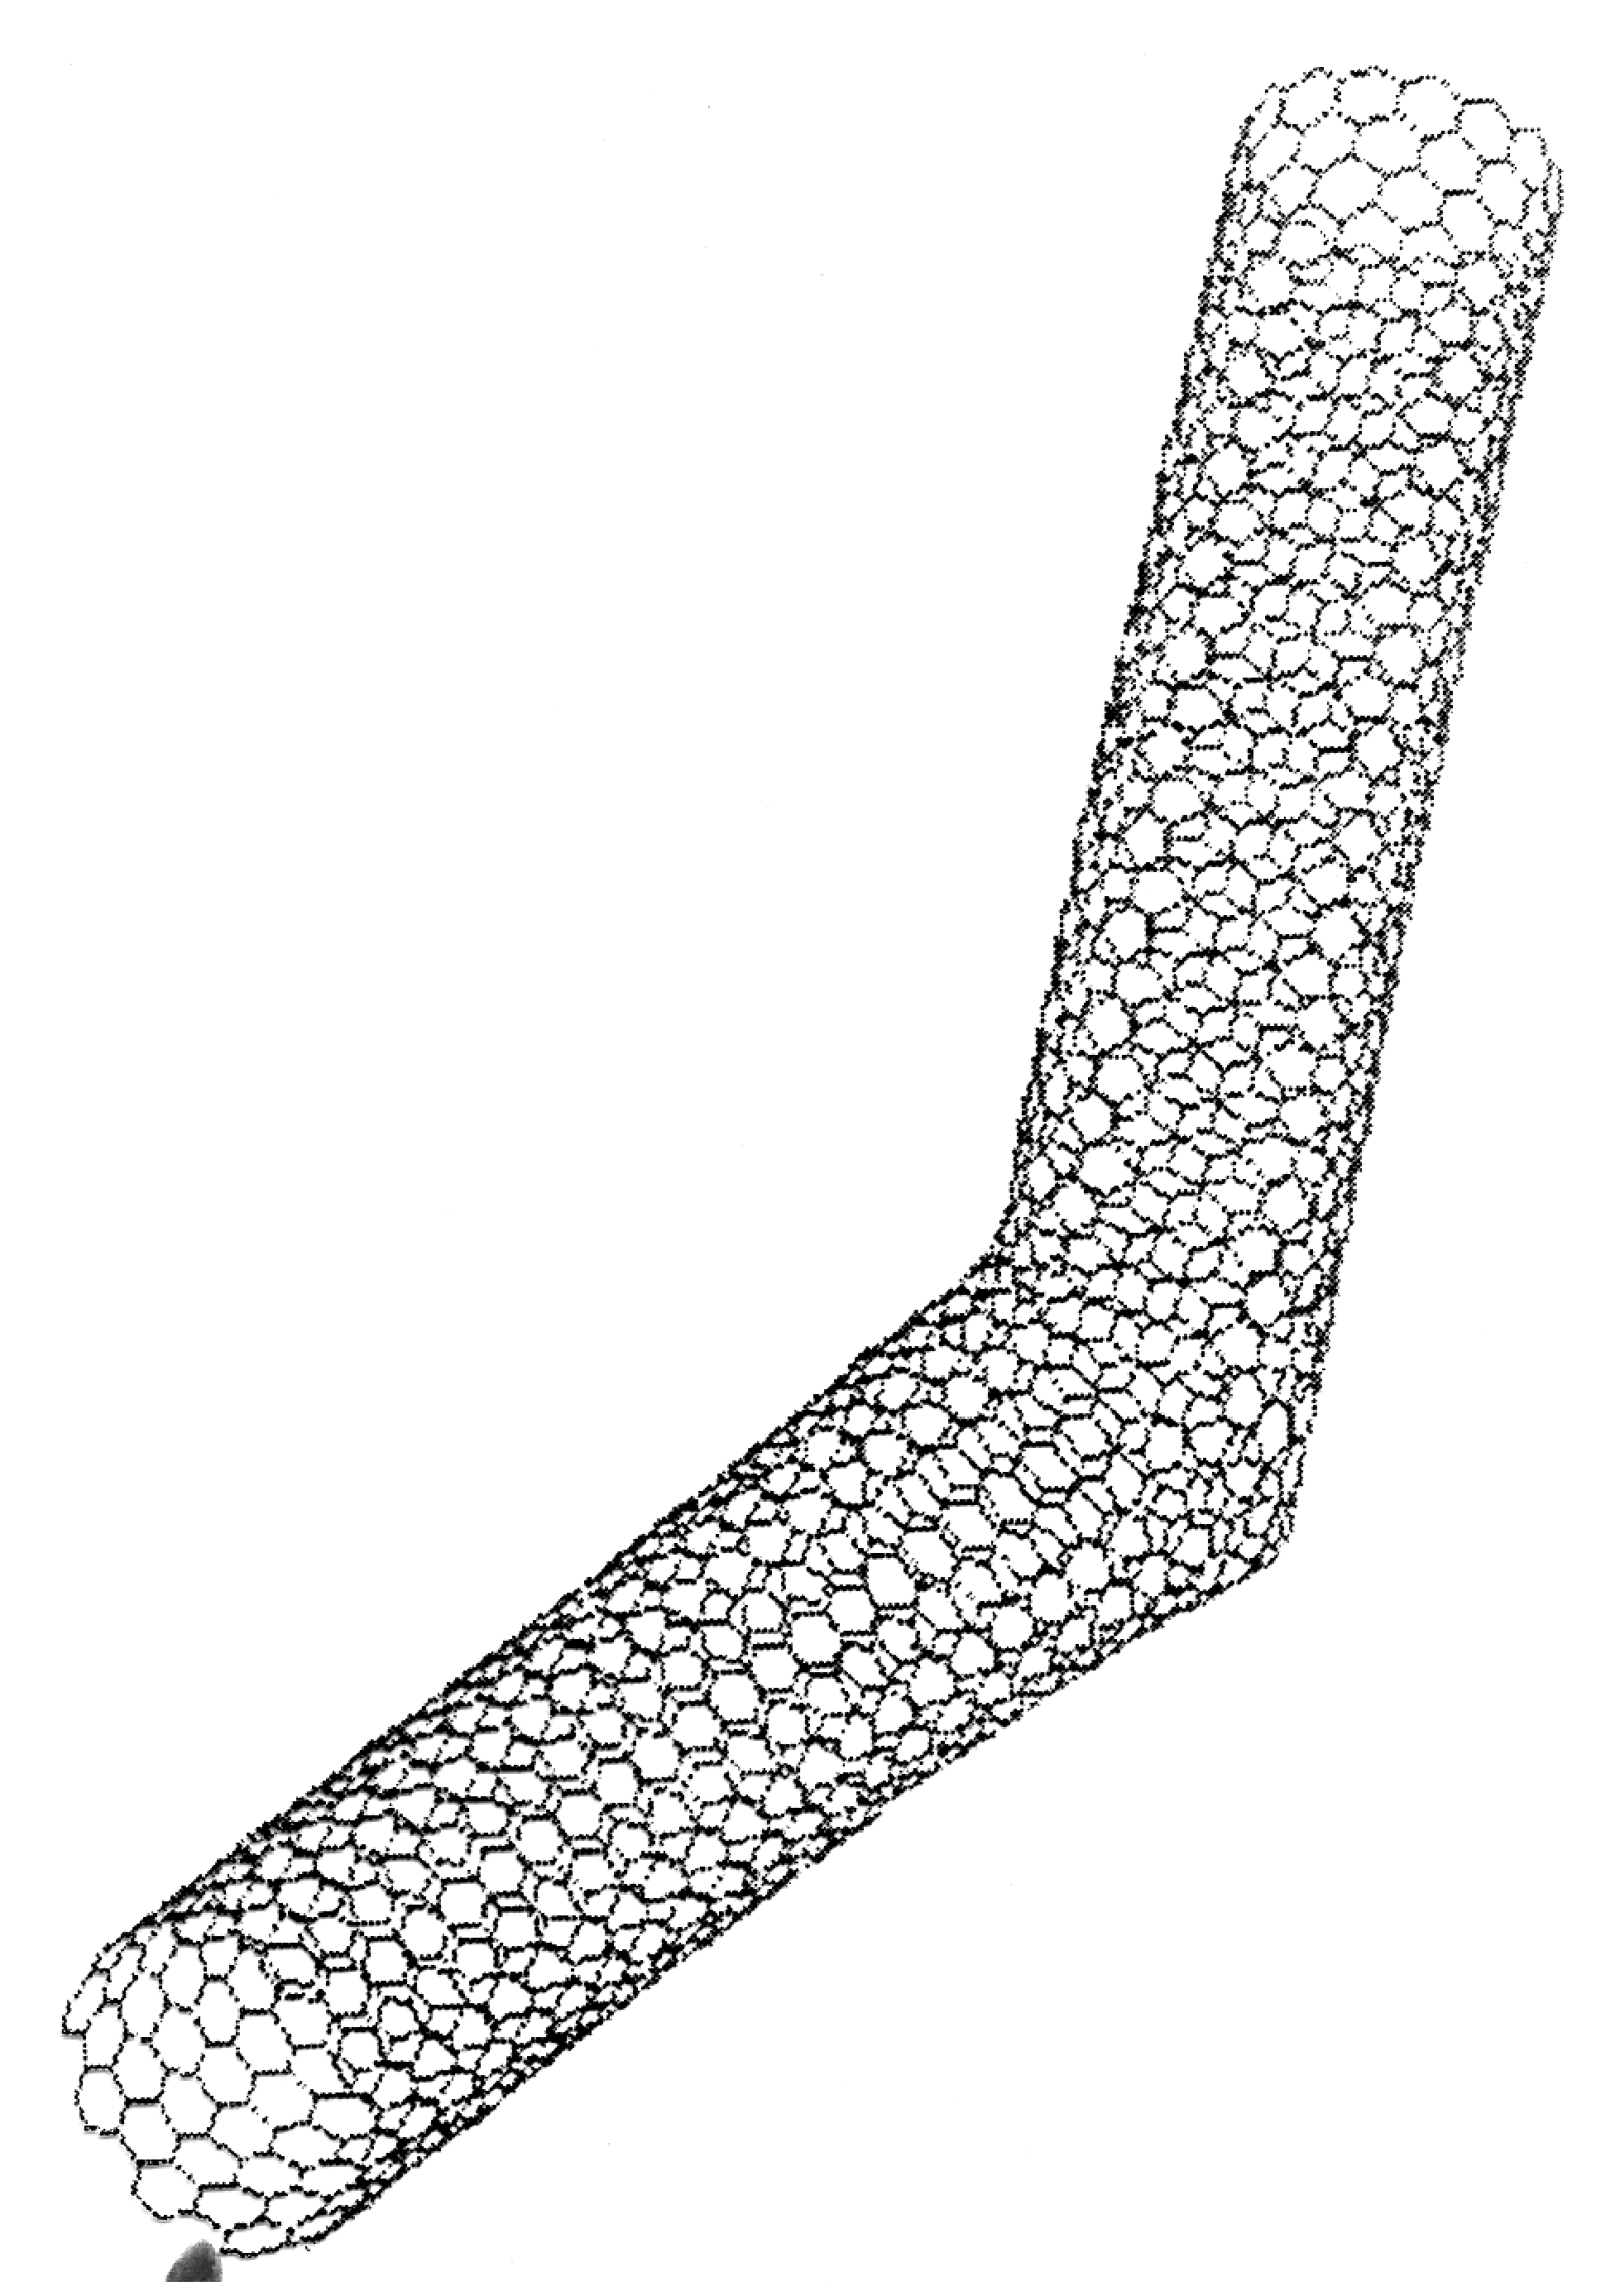
\includegraphics{DRAW/ScanDezaPres/pic2.eps}}\par
Deformed graphite tube
\end{minipage}
\end{center}

\begin{center}
Nested tubes (concentric cylinders) of rolled graphite;\\
use(?): for composites and ``nanowires''
\end{center}
\end{slide}


\begin{slide}{Other possible applications}
\begin{itemize}
\item \textcolor{red}{Superconductors:} alcali-doped fullerene compounds
$K_3C_{60}$ at $18K$,\dots, $Rb_3C_{60}$ at $30K$\\
but still too low transition $T_c$
\item \textcolor{red}{HIV-1}: Protease Inhibitor since
derivatives of $C_{60}$ are highly hydrophobic and have large 
size and stability;
\par 2003: drug design based on antioxydant property of 
fullerenes (they soak cell-damaging free radicals)
\item \textcolor{red}{Carbon nanotubes}
\begin{itemize}
\item ? superstrong materials
\item ? nanowires
\item ! already soon: sharper scanning microscope
\end{itemize}
\end{itemize}
But nanotubes are too expensive at present
\end{slide}




\begin{slide}{Chemical context}
\begin{itemize}
\item \textcolor{red}{Crystals}: from basic units by symm. operations, incl. 
\textcolor{blue}{translations}, excl. \textcolor{blue}{order $5$ 
rotations} (``cryst. 
restriction'').\\
Units: from few (inorganic) to thousands (proteins).
\item Other very symmetric mineral structures: \textcolor{red}{quasicrystals}, 
fullerenes and like, icosahedral packings (no translations but rotations 
of order $5$)
\item Fullerene-type polyhedral structures (polyhedra, nanotubes, cones, saddles, \dots) were first observed with carbon.
But also inorganic ones were considered: boron nitrides, tungsten, 
disulphide,
allumosilicates and, possibly, fluorides and chlorides.

May 2006, Wang-Zeng-al.: first \textcolor{red}{metal hollow cages}
$Au_n=F^{*}_{2n-4}$ ($16 \le n \le18$). $F^{*}_{28}$ is the smallest; 
the gold 
clusters are 
flat if $n<16$ and compact (solid) if $n>18$.


\end{itemize}

\end{slide}



\begin{slide}{Stability}
Minimal total energy:
\begin{itemize}
\item $I$-energy and
\item the strain in the $6$-system.
\end{itemize}
H\"uckel theory of $I$-electronic structure: every eigenvalue $\lambda$ of the adjacency matrix of the graph corresponds to an orbital of energy $\alpha+\lambda \beta$.

$\alpha$: Coulomb parameter (same for all sites)

$\beta$: resonance parameter (same for all bonds)

The best $I$-structure: same \# of positive and negative eigenvalues 

%NEED TO FIND PAPER DETAILING THOSE NOTIONS.
\end{slide}

\begin{slide}{Skyrmions and fullerenes}
{\bf Conjecture} (Sutcliffe et al.):\\
any minimal energy Skyrmion (baryonic density isosurface for
single soliton solution) with baryonic number (the number of nucleons)
$B \ge 7$ is a fullerene $F_{4B-8}$.

{\bf Conjecture} (true for $B<107$; open from $(b,a)=(1,4)$):\\
there exist \textcolor{blue}{icosahedral} minimal energy Skyrmion for
any $B=5(a^2+ab+b^2)+2$ with integers $0 \le b <a$, $gcd(a,b)=1$
(not any icosahedral Skyrmion has minimal energy).

\vspace{3mm}
Skyrme model (1962) is a Lagrangian approximating $QCD$ (a gauge theory 
based on $SU(3)$ group). Skyrmions are special topological solitons used to 
model baryons.   

\end{slide}




\begin{slide}{Life fractions}
\begin{itemize}
\item \textcolor{red}{life}: DNA and RNA (cells)
\item \textcolor{red}{$1/2$-life}: DNA or RNA (cell parasites: viruses)
\item ``naked'' RNA, no protein (satellite viruses, viroids)
\item  DNA, no protein (plasmids, nanotech, ``junk'' DNA, ...)
\item \textcolor{red}{no life}: no DNA, nor RNA  (only proteins, incl. prions)
\end{itemize}
{\small
\begin{tabular}{c|c|c|c|c|c}
          &Atom   &DNA        &Cryo-EM    &Prion  &Viruses\\
\hline
size  &0.2-0.3 &$\simeq 2$&$\simeq 5$ &$11$   &$20-50-100-400$\\
nm   &        &          &           &       &B-19,  HIV, Mimi
\end{tabular}
}
Virion: protein capsid (or env.spikes) icosadeltahedron
$C_{20T}^*$, $T=a^2+ab+b^2$ (triangulation number)

\end{slide}






\begin{slide}{Digression on viruses}
\begin{tabular}{|c|c|c|}
\hline
life          &$1/2$-life    &\dots viroids \dots non-life\\
\hline
DNA \textcolor{red}{and} RNA   &DNA \textcolor{red}{or} RNA    &neither DNA, \textcolor{red}{nor} RNA\\
\hline
Cells         &Viruses       &Proteins, incl. prions\\
\hline
\end{tabular}
Seen in 1930 (electronic microscope): tobacco mosaic.\\
$1mm^3$ of seawater has $\simeq 10 $ million viruses; all seagoing viruses 
$\simeq 270$ million tons (more 20 x weight of all whales).

\textcolor{blue}{Origin}: ancestors or vestiges of cells, or gene mutation? 
%or, $>3.5$ billion years ago, DNA 
%in early cells was not organized into chromosomes yet; protein, by gene 
%mutation, self-assembled into icosahedral shells: 
%``primitive virus'' (a DNA segment trapped in protein)

Or, evolved in parallel with cellular forms from
self-replicating molecules in prebiotic ``RNA world"\\
Virus: \textcolor{blue}{virion}, then (rarely) cell parasite\\
Virion: capsid (protein coat), capsomers structure\\

Number of protein subunits is $60T$, but EM
resolves only clusters-``capsomers'' ($12T+2$ vertices of
$C_{20T}^*$), including $12$ ``pentamers'' ($5$-valent vertices)
at minimal distance $a+b$

%Other bio. structures, forming fullerenes: clathrin coated vesicles
%(in eukaryote cells)
\end{slide}







\begin{slide}{}
1954, Watson and Crick conjectured: symmetry is cylindrical or 
icosahedral
(i.e. dual $I$, $I_h$ fullerenes). It holds, and almost all DNA and 
dsRNA 
viruses with known shape are icosahedral.\\
\vspace{3mm}
AIDS: icosahedral, but $(a,b)$? Plant viruses? Chirality?
nm: $1$ typical molecule; $20$ Parvovirus $B$-$19$, $400$ Mimivirus;

150 ``minimal cell'' (bacterium Micoplasma genitalium);

90 smallest feature of computer chip (= diam. HIV-1).\\
\vspace{3mm}
Main defense of multi-cellular organism, sexual reproduction, 
is not effective (in cost, risk, speed) but arising mutations 
give some chances against viruses.

%of viruses and gene exchange between bacteria 
\end{slide}



\begin{slide}{Capsids of viruses}
{\tiny
\begin{center}
\begin{tabular}{||c||c|c||}
\hline
\hline
$(a,b)$ & Fullerene & Virus capsid (protein coat)\\
\hline
$(1,0)$ & $F_{20}^*(I_h)$ & {\it Gemini virus} \\
$(1,1)$ & $C_{60}^*(I_h)$ & {\it turnip yellow mosaic virus} \\
$(2,0)$ & $C_{80}^*(I_h)$ & {\it hepatitis B, Bacteriophage $\Phi R$}\\
$(2,1)$ & $C_{140}^*(I)_{laevo}$ & {\it HK97, rabbit papilloma virus} \\
$(1,2)$ & $C_{140}^*(I)_{dextro}$ & {\it human wart virus} \\
%$(3,0)$ & $C^*_{180}(I_h)$ & {\it Outer shell of reovirus} \\ \hline
$(3,1)$ & $C_{200}^*(I)_{laevo}$ & {\it rotavirus} \\
$(4,0)$ & $C_{320}^*(I_h)$ & {\it herpes virus, varicella} \\
$(5,0)$ & $C_{500}^*(I_h)$ & {\it adenovirus} \\
$(6,0)$ & $C_{720}^*(I_h)$ & {\it infectious canine hepatitis virus, HTLV-1}\\
$(9,0)$ & $C_{1620}^*(I_h)$ & {\it Tipula virus} \\
$(6,3)$? & $C_{1260}^*(I)_{laevo}$ & {\it HIV-1}\\
$(7,7)$? & $C_{2940}^*(I_h)$ & {\it iridovirus}\\ 
\hline
\hline
\end{tabular}
\end{center}
}
\end{slide}


\begin{slide}{Some viruses}
\begin{center}
\begin{minipage}[b]{5.5cm}
\centering
\resizebox{4.5cm}{!}{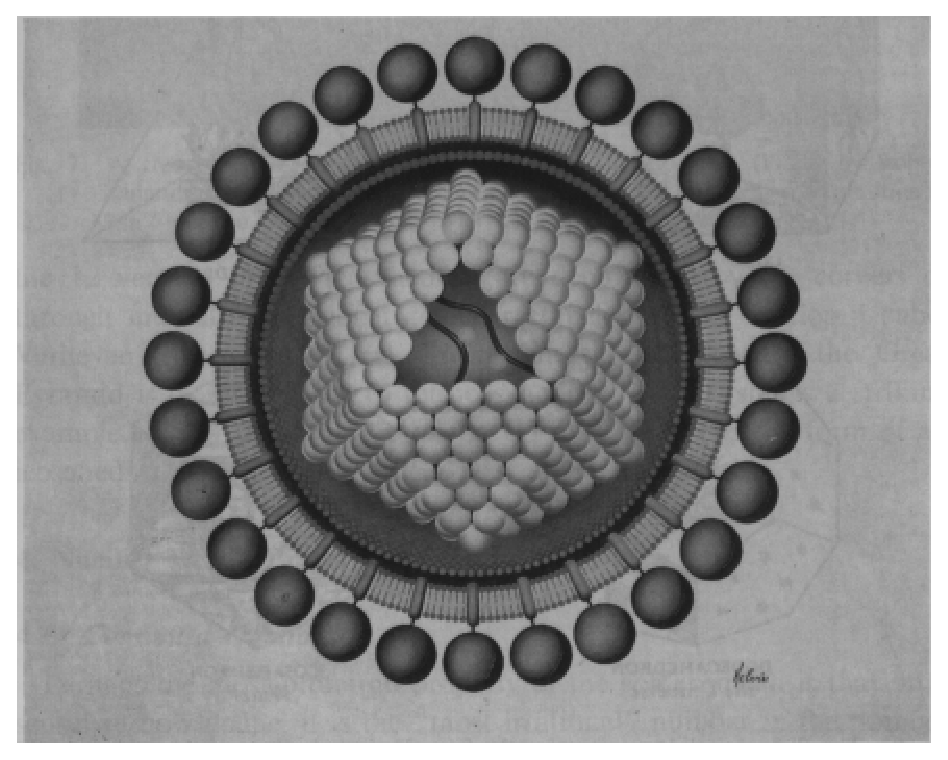
\includegraphics{DRAW/PS/aids.ps}}\par
Icosadeltahedron $C_{720}^*(I_h)$,\\
the icosahedral structure of the HTLV-1
\end{minipage}
\hspace{0.1cm}
\begin{minipage}[b]{5.5cm}
\centering
\resizebox{3.5cm}{!}{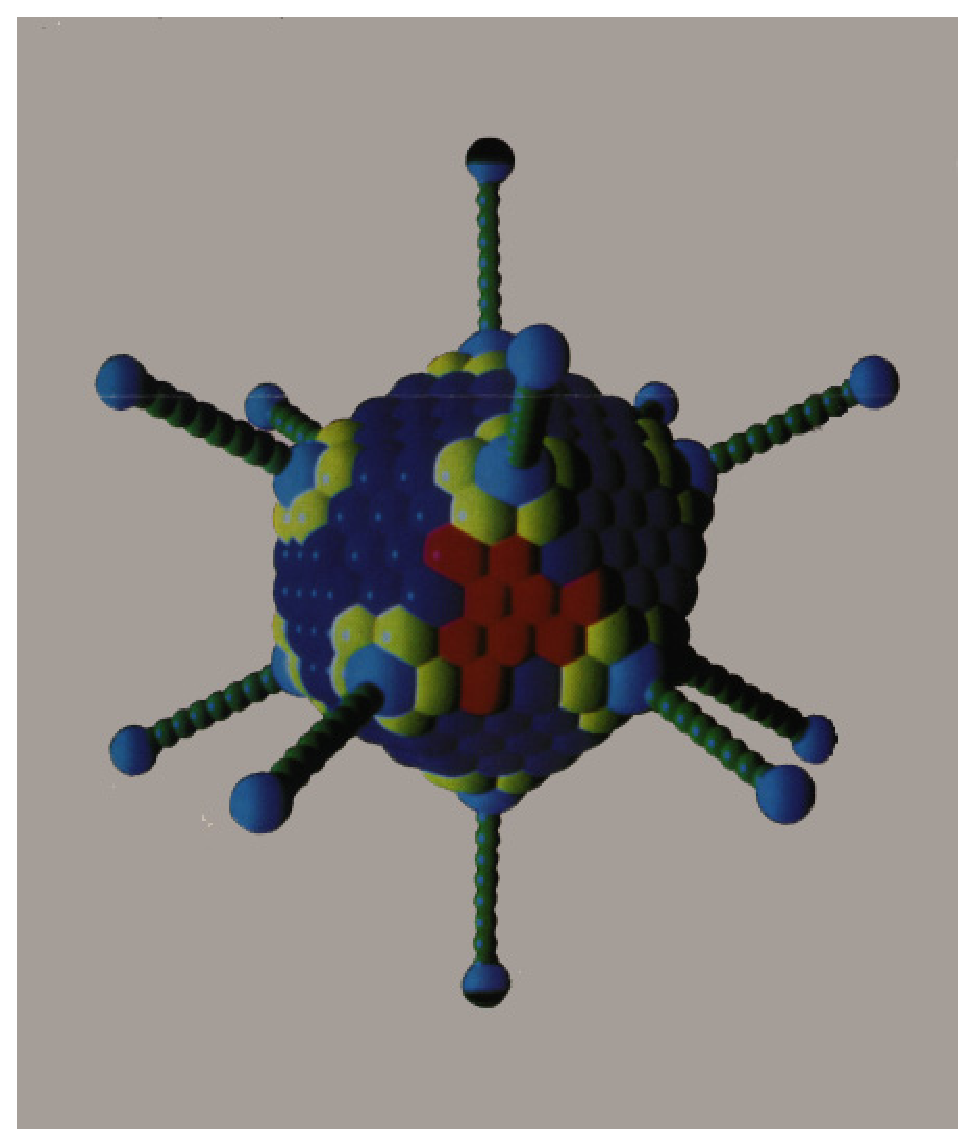
\includegraphics{DRAW/PS/virus.ps}}\par
Simulated adenovirus $C_{500}^*(I_h)$ with its spikes
$(5,0)$-dodecahedron $C_{500}(I_h)$
\end{minipage}
\end{center}

\end{slide}





\begin{slide}{}
\begin{center}
{\Huge 
\begin{tabular*}{6cm}{c}
\\[-0.5cm]
\textcolor{blue}{IV. }\textcolor{red}{Some}\\
\textcolor{red}{fullerene-like}\\
\textcolor{red}{3-valent maps}
\end{tabular*}
}
\end{center}
\end{slide}





\begin{slide}{Mathematical chemistry}
use following fullerene-like $3$-valent maps:
\begin{itemize}
\item Polyhedra $(p_5, p_6, p_n)$ for $n=4$, $7$ or $8$ ($v_{min}=14$, $30$, $34$) Aulonia hexagona (E. Haeckel 1887): plankton skeleton
\item \textcolor{blue}{Azulenoids} $(p_5, p_7)$ on torus $g=1$; so, $p_5=p_7$\par
azulen \resizebox{1.5cm}{!}{\includegraphics{Boundary/Azulene.eps}} is an isomer $C_{10}H_{8}$ of naftalen \resizebox{1.5cm}{!}{\includegraphics{Polycycle/ris-1bis-b.eps}}
\end{itemize}

%\begin{center}
%{\bf Toric azulenoids}
%\end{center}

\begin{center}
\begin{minipage}[b]{5.5cm}
\centering
\resizebox{4.5cm}{!}{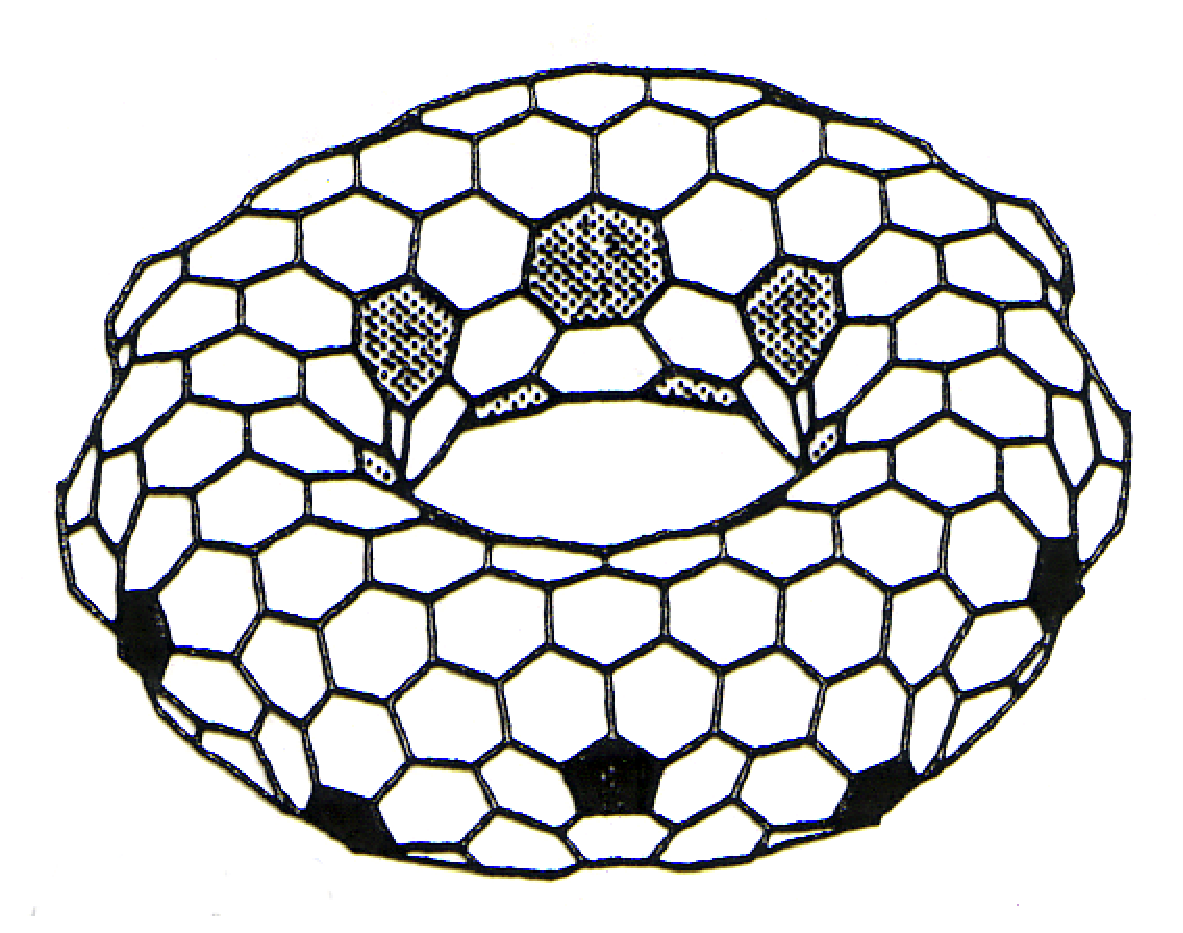
\includegraphics{DRAW/ScanDezaPres/pic6.eps}}\par
%\textcolor{white}{Bonjour}\\
%\textcolor{white}{Bonjour}
\end{minipage}
\hspace{0.1cm}
\begin{minipage}[b]{5.5cm}
\centering
\resizebox{3.5cm}{!}{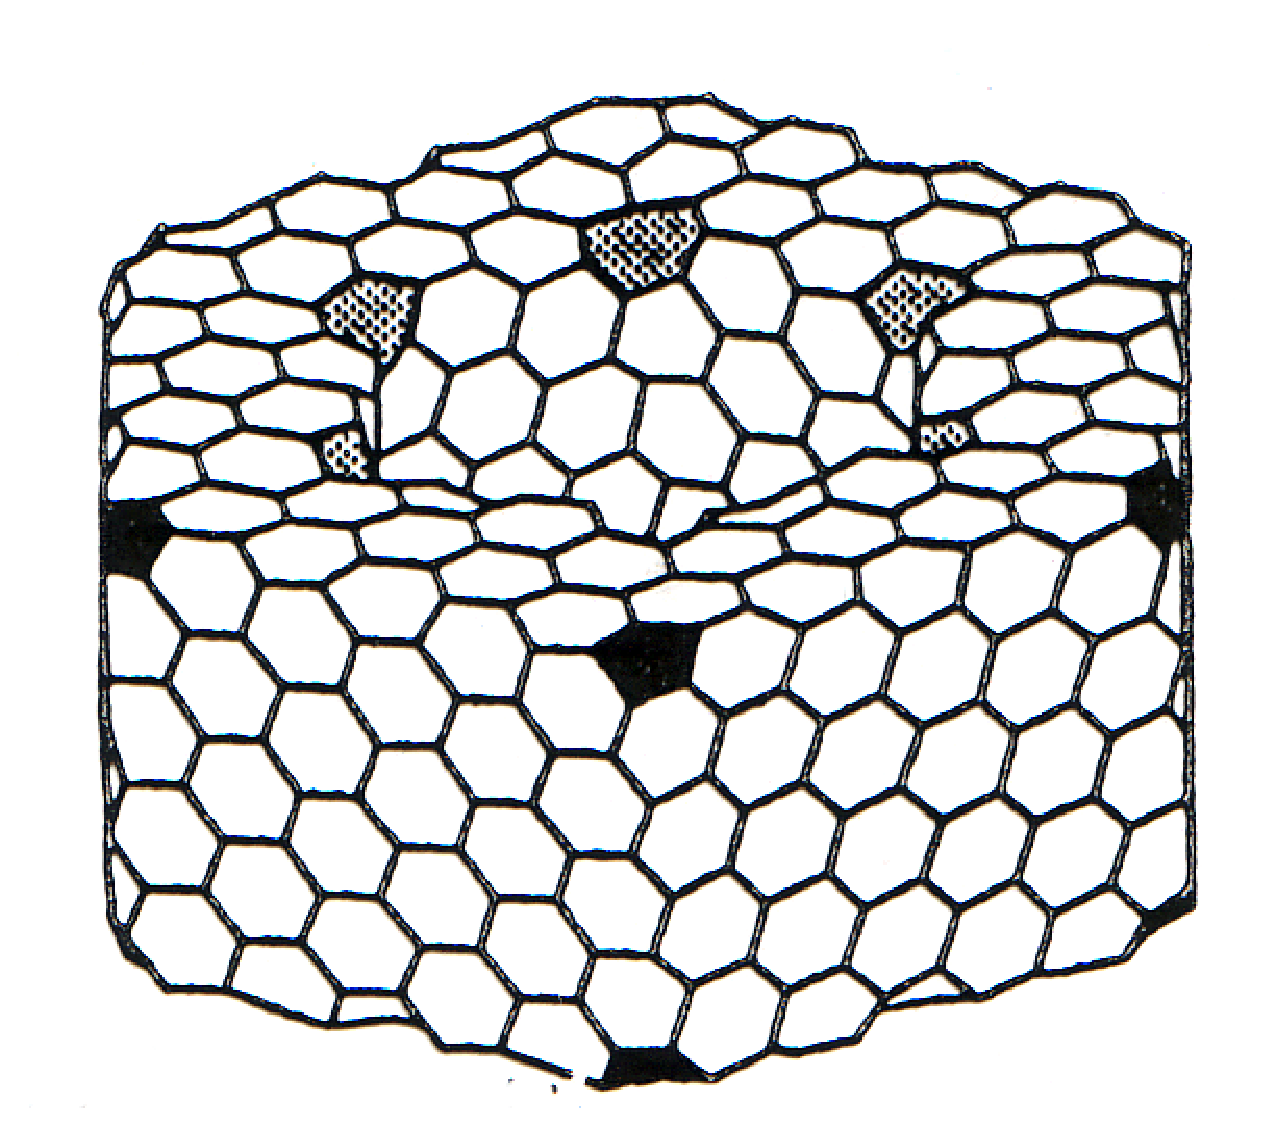
\includegraphics{DRAW/ScanDezaPres/pic5.eps}}\par
$(p_5, p_6, p_7)=(12, 142, 12)$, $v=432$, $D_{6d}$
\end{minipage}
\end{center}



\end{slide}


\begin{slide}{Schwarzits}
\vspace{-3mm}
\textcolor{blue}{Schwarzits} $(p_6, p_7, p_8)$ on minimal surfaces of constant negative curvature ($g\geq 3$). We consider case $g=3$:\\

\begin{center}
\begin{minipage}[b]{5.5cm}
\centering
\resizebox{3.3cm}{!}{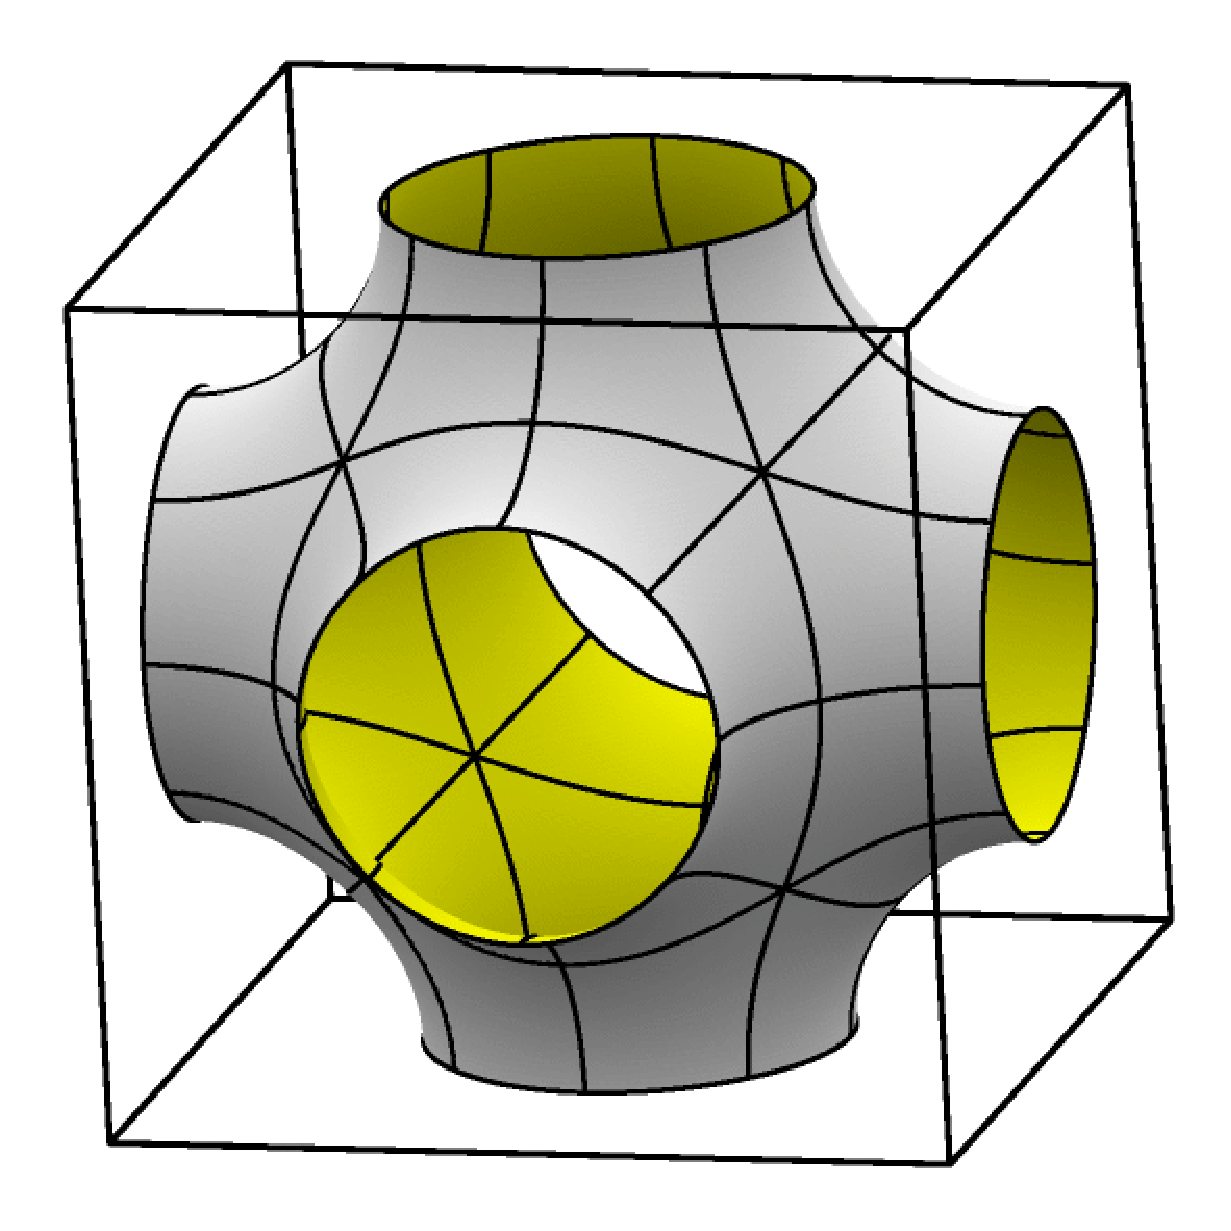
\includegraphics{FullPresPic/pcube.8.eps}}\par
Schwarz $P$-surface
\end{minipage}
\begin{minipage}[b]{5.5cm}
\centering
\resizebox{3.3cm}{!}{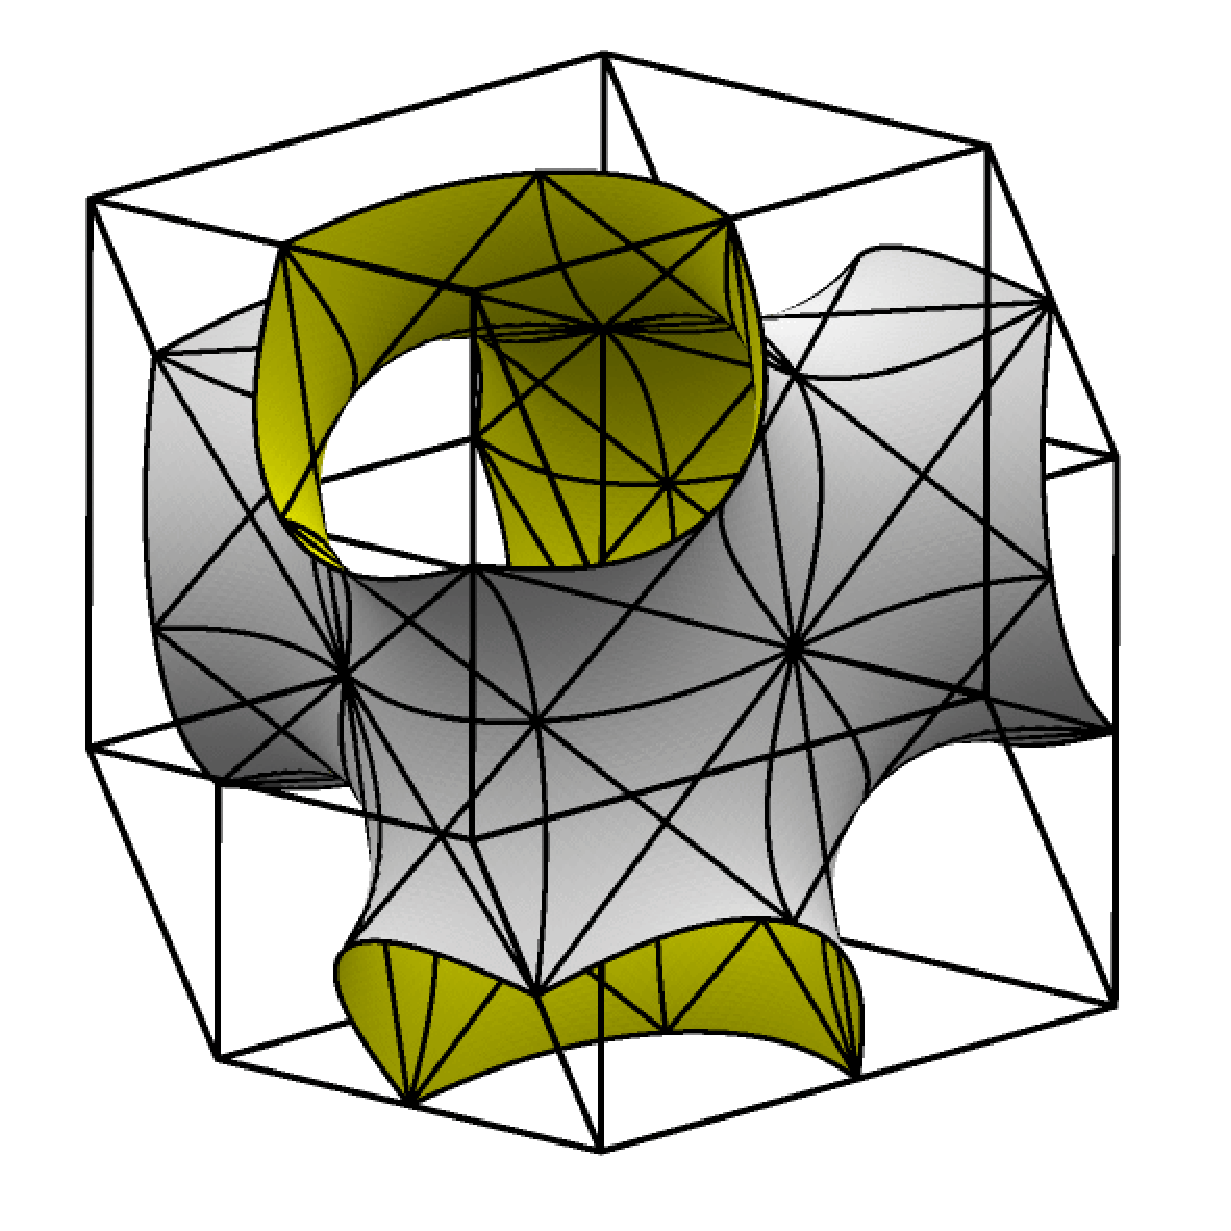
\includegraphics{FullPresPic/drhomb.8.eps}}\par
Schwarz $D$-surface
\end{minipage}
\end{center}

\begin{itemize}
\item We take a $3$-valent genus $3$-map and cut it along zigzags \resizebox{2.0cm}{!}{\includegraphics{FullPresPic/Zigzag.eps}} and paste it to form $D$- or $P$-surface.
\item We need $3$ non-intersecting zigzags. For example, Klein-map has $5$ types of such triples.
\end{itemize}

%Examples (for $g=3$) on $D$- or $P$-surface (``plumber's 
%nightmare'' - $3$ hyperboloids with axes intersecting at right angles): 
%$(p_6,24,0)$ and $(p_6,0,12)$.


\end{slide}



%^

%\begin{slide}{Toric azulenoids}

%\begin{center}
%$(p_5, p_6, p_7)=(12, 142, 12)$, $v=432$ $D_{6d}$, toric azulenoids
%\end{center}
%\end{slide}



\begin{slide}{$(6,7)$-surfaces}
\begin{center}
\begin{minipage}[b]{3.7cm}
\centering
\resizebox{3.0cm}{!}{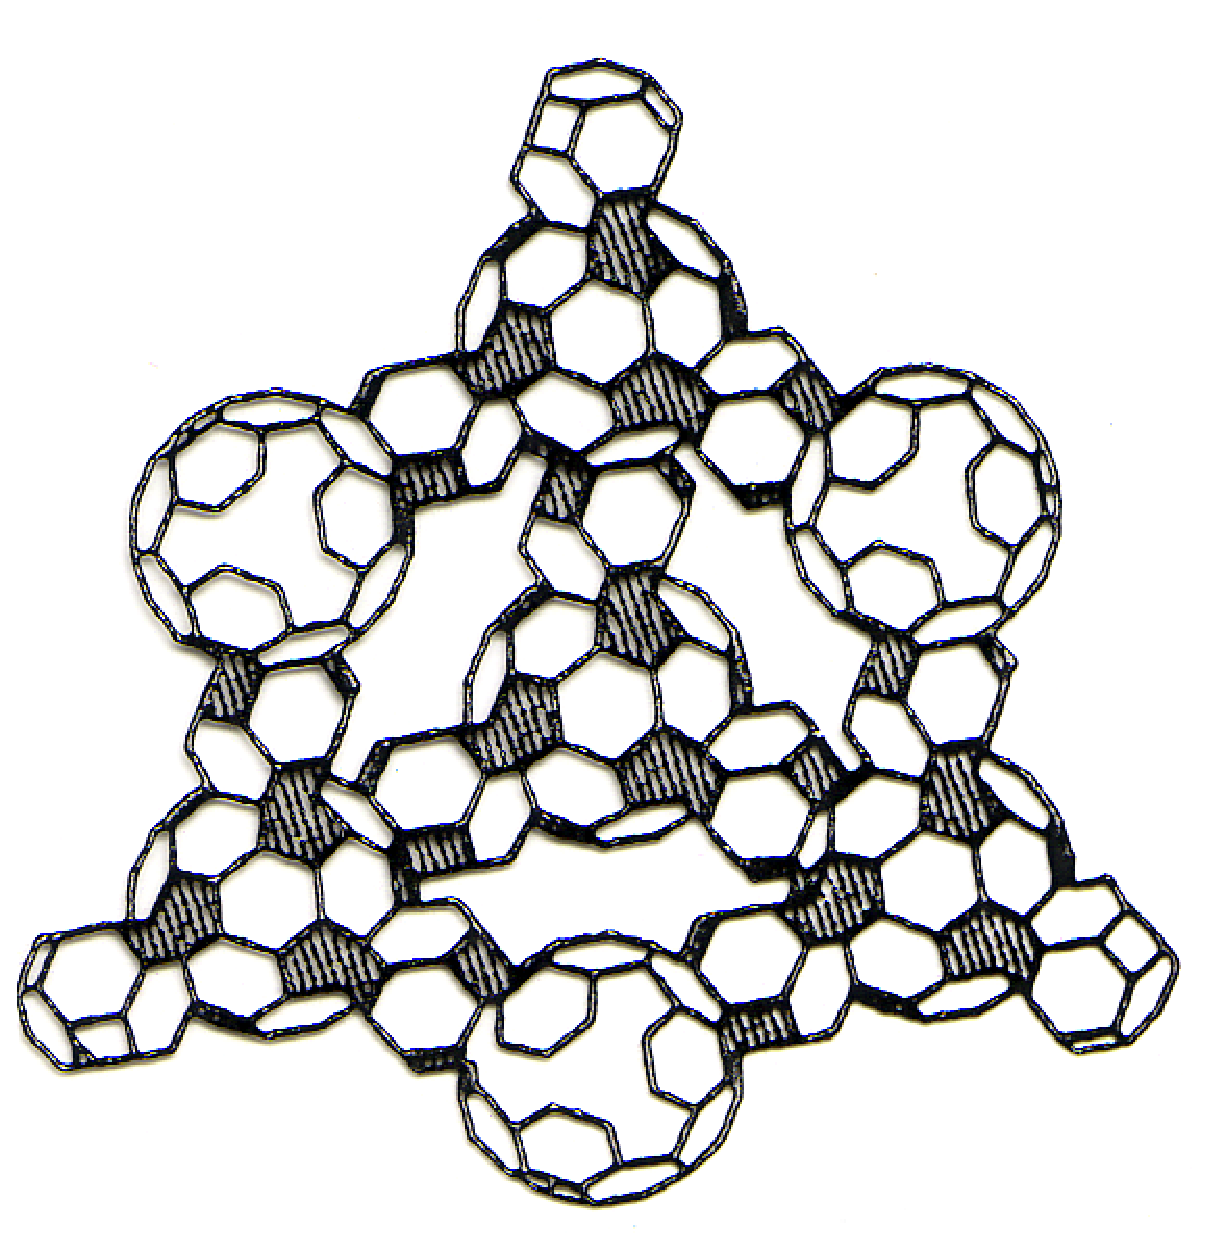
\includegraphics{DRAW/ScanDezaPres/pic10.eps}}\par
$(1,1)$\par
$D168$: putative carbon, 1992, (Vanderbilt-Tersoff)
\end{minipage}
\begin{minipage}[b]{3.7cm}
\centering
\resizebox{3.2cm}{!}{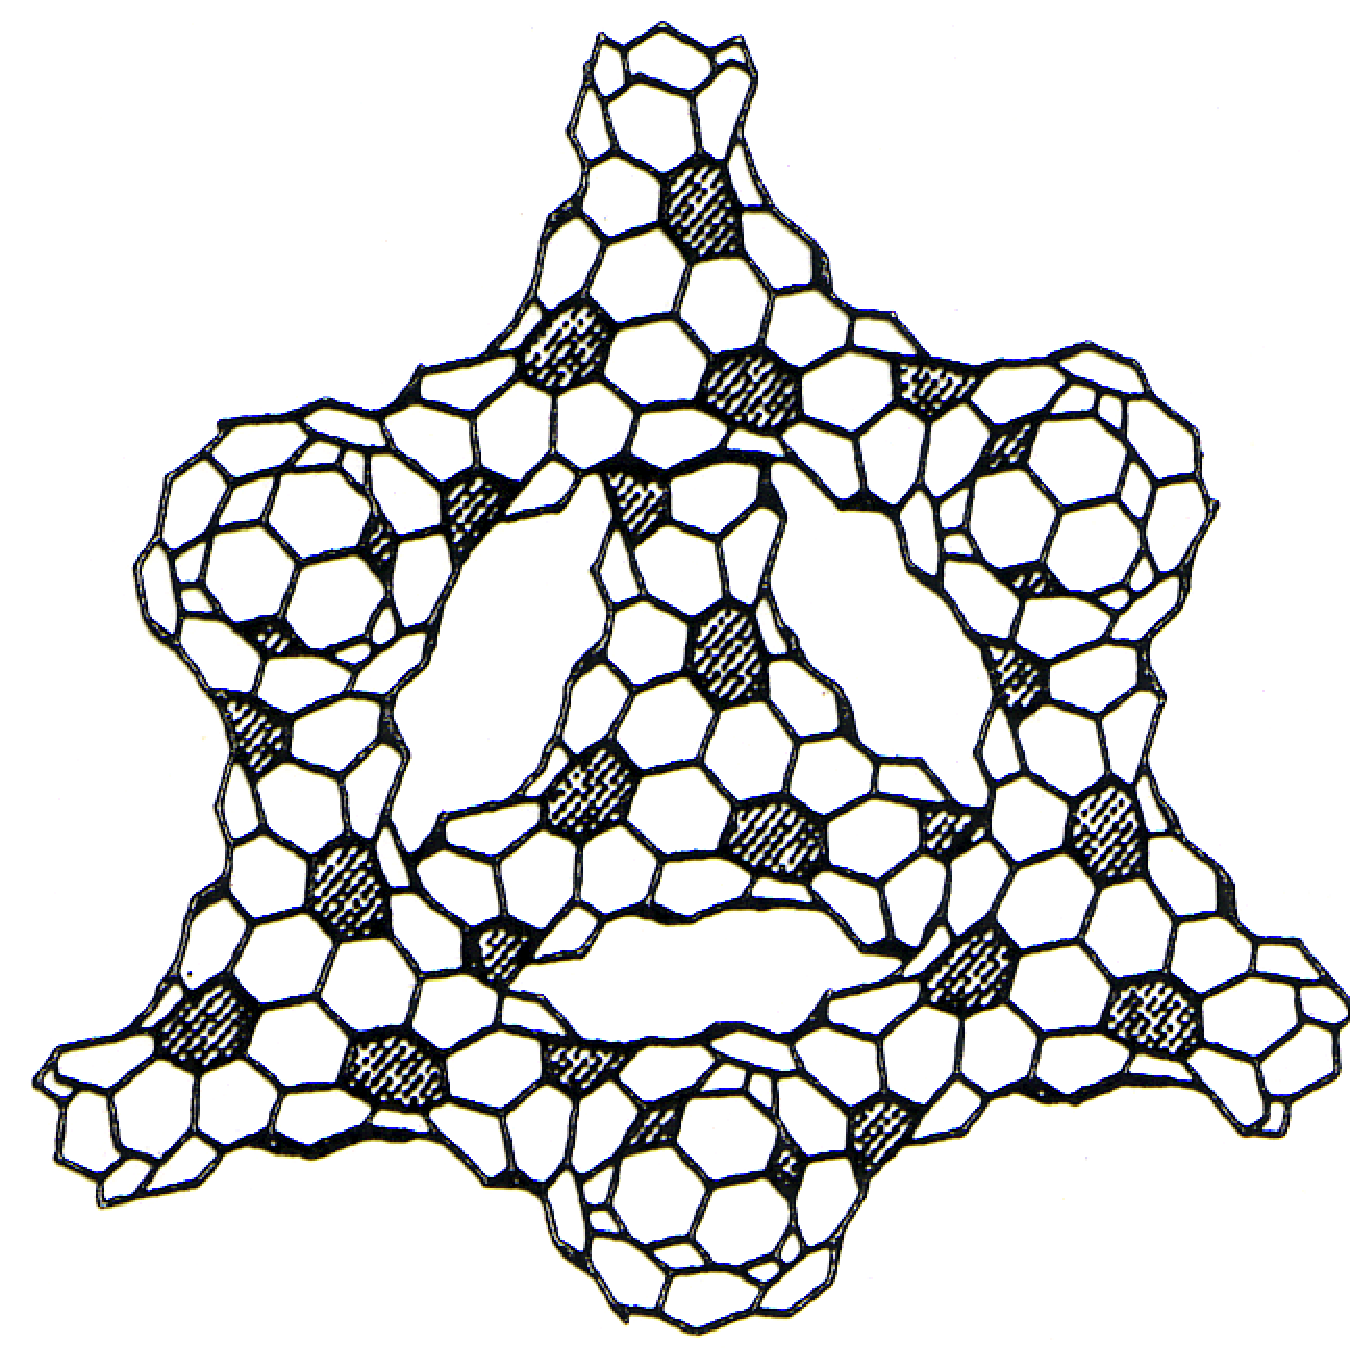
\includegraphics{DRAW/ScanDezaPres/pic11.eps}}\par
$(0,2)$\\
\textcolor{white}{Bonjour}
\end{minipage}
\begin{minipage}[b]{3.7cm}
\centering
\resizebox{3.6cm}{!}{\includegraphics{DRAW/ScanDezaPres/pic12.eps}}\par
$(1,2)$\\
\textcolor{white}{Bonjour}
\end{minipage}
\end{center}

\begin{center}
$(p_6, p_7=24)$, $v=2p_6+56=56(p^2+pq+q^2)$\par
Unit cell of $(1,0)$: $D56$ - Klein regular map $(7^3)$

\end{center}
\end{slide}




\begin{slide}{$(6,8)$-surfaces}
\begin{center}
\begin{minipage}[b]{3.7cm}
\centering
\resizebox{3.0cm}{!}{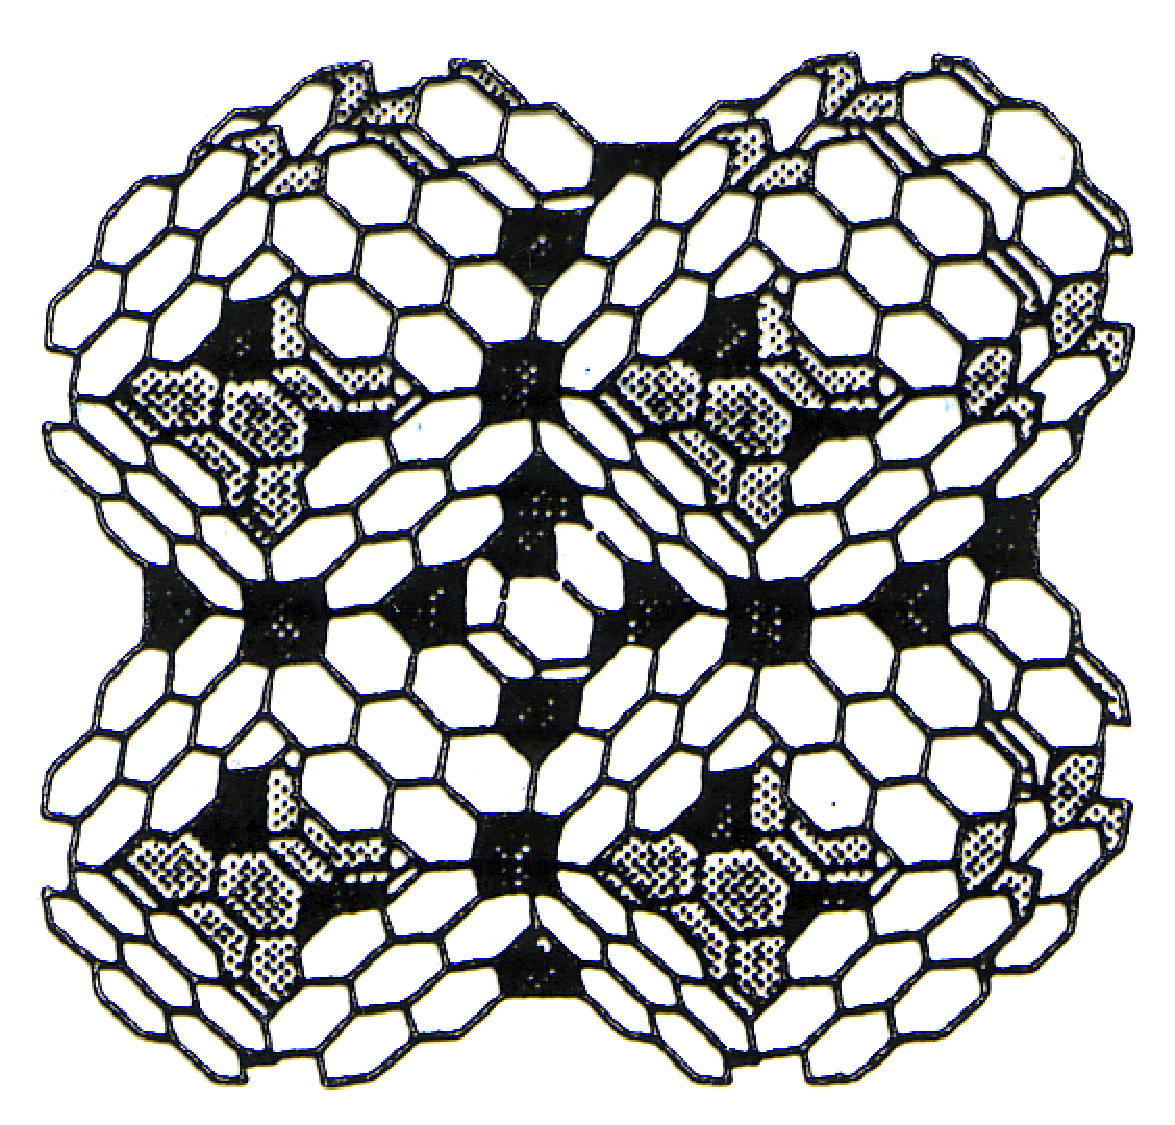
\includegraphics{DRAW/ScanDezaPres/pic7.eps}}\par
$(1,1)$\\
\textcolor{white}{Bonjour}
\end{minipage}
\begin{minipage}[b]{3.7cm}
\centering
\resizebox{3.2cm}{!}{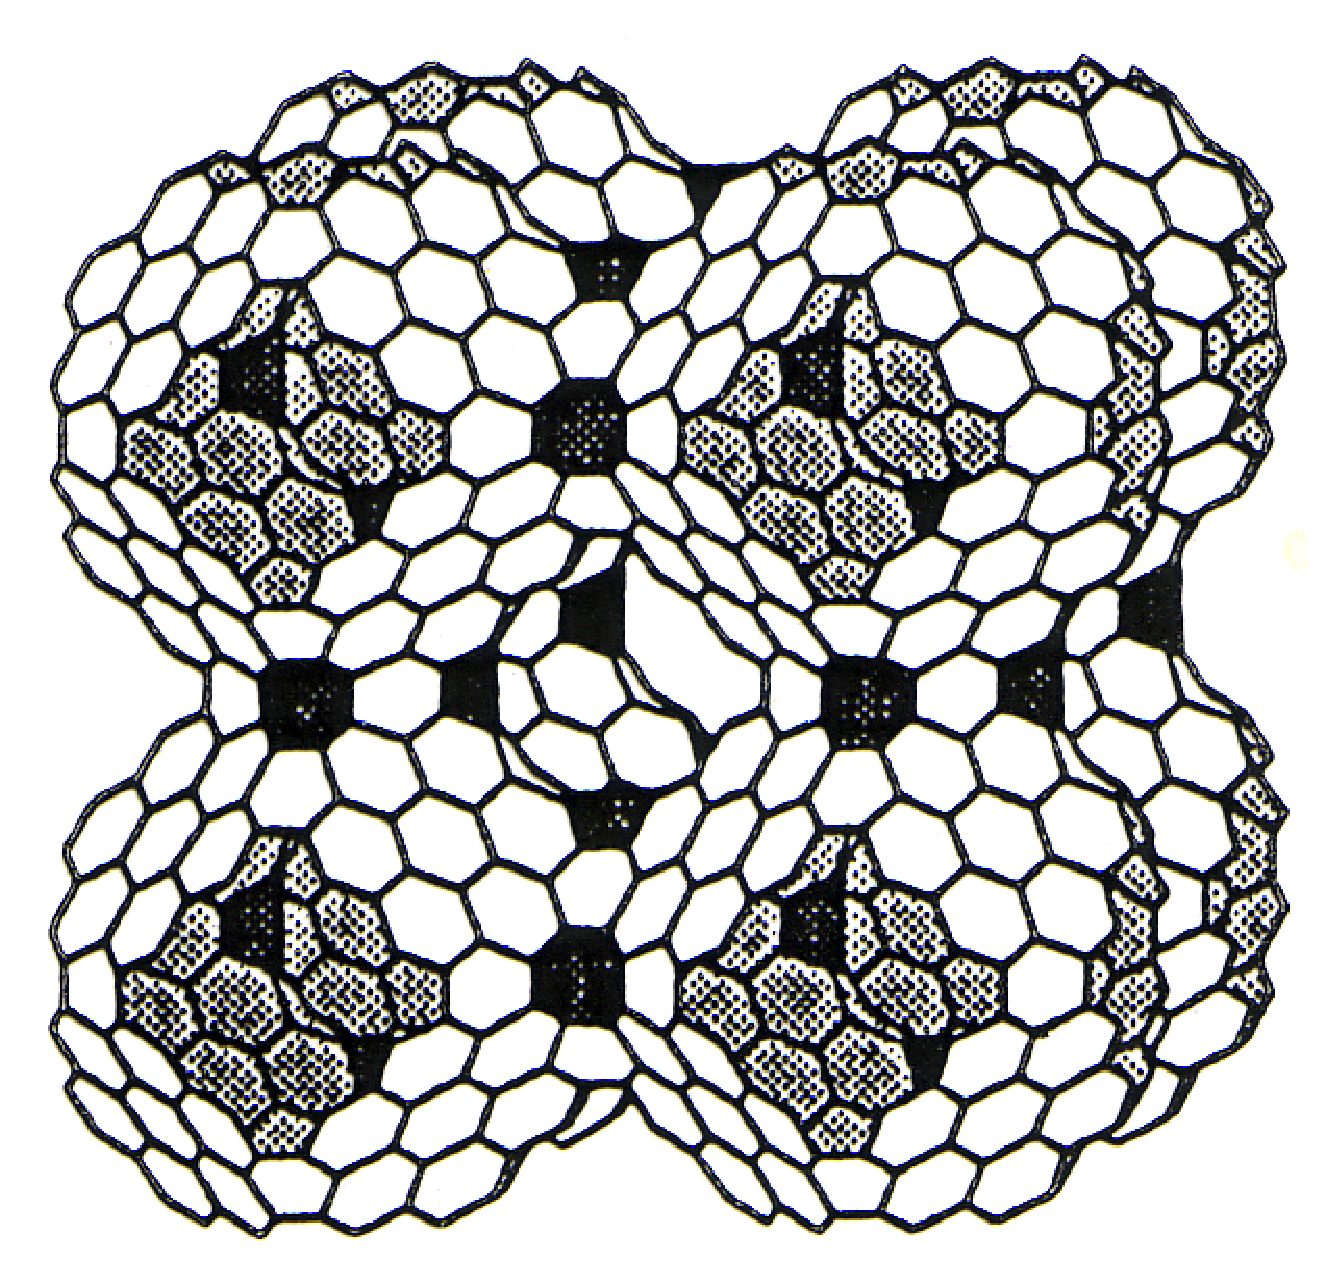
\includegraphics{DRAW/ScanDezaPres/pic8.eps}}\par
$(0,2)$\par
$P192$, $p_6=80$
\end{minipage}
\begin{minipage}[b]{3.7cm}
\centering
\resizebox{3.6cm}{!}{\includegraphics{DRAW/ScanDezaPres/pic9.eps}}\par
$(1,2)$\\
\textcolor{white}{Bonjour}
\end{minipage}
\end{center}

\begin{center}
$(p_6, p_8=12)$, $v=2p_6+32=48(p^2+pq+q^2)$\par
$(1,0)$: $p_6=2$ \par
Unit cell of $p_6=0$: $v=32$ - Dyck regular map $(8^3)$
\end{center}
\end{slide}






\begin{slide}{More $(6,8)$-surfaces}
\begin{center}
\begin{minipage}[b]{5.5cm}
\centering
\resizebox{4.6cm}{!}{\includegraphics{DRAW/ScanDezaPres/pic13.eps}}\par
$(0,2)$\\
$v=120$, $p_6=44$
\end{minipage}
\begin{minipage}[b]{5.5cm}
\centering
\resizebox{4.6cm}{!}{\includegraphics{DRAW/ScanDezaPres/pic14.eps}}\par
$(1,2)$\\
\textcolor{white}{Bonjour}
\end{minipage}
\end{center}

\begin{center}
$(p_6, p_8=12)$, $v=2p_6+32=30(p^2+pq+q^2)$\par
Unit cell of $p_6=0$: $v=32$ - Dyck regular map $(8^3)$
\end{center}

\end{slide}


\begin{slide}{Polycycles (with Dutour and Shtogrin)}
A finite \textcolor{red}{$(p,q)$-polycycle}  is a plane $2$-connected finite graph, such that :

\begin{itemize}
\item all interior faces are (combinatorial) $p$-gons,
\item all interior vertices are of degree $q$,
\item all boundary vertices are of degree in $[2,q]$.
\end{itemize}

\begin{center}
\epsfig{file=Boundary/3_5_polycycle.eps, width=4cm}\par
a $(5,3)$-polycycle
\end{center}
%All polycycles considered have $s=3$ and are finite.

\end{slide}

\begin{slide}{Examples of $(p,3)$-polycycles}
\begin{itemize}
\item $p=3$: $\{3,3\}$, $\{3,3\}-v$, $\{3,3\}-e$;
\item $p=4$: $\{4,3\}$, $\{4,3\}-v$, $\{4,3\}-e$, $P_2\times A$ ($A=P_{n\geq 1}$, $P_{\NN}$, $P_{\ZZ}$)
\item Continuum for any $p\geq 5$.\\
But $39$ \textcolor{blue}{proper} $(5,3)$-polycycles, i.e., partial subgraphs of Dodecahedron
\item $p=6$: polyhexes=benzenoids
\end{itemize}
{\bf Theorem}\\
(i) Planar graphs admit at most one realization as $(p,3)$-polycycle\\
(ii) any unproper $(p,3)$-polycycle is a \textcolor{blue}{$(p,3)$-helicene}\\
(homomorphism into the plane tiling $\{p,3\}$ by regular
$p$-gons)
\end{slide}









\begin{slide}{Icosahedral fulleroids (with Delgado)}

\begin{itemize}
\item $3$-valent polyhedra with $p=(p_5, p_{n>6})$ and symmetry $I$ or $I_h$
\end{itemize}


\begin{center}
\begin{tabular}{|c|c|c|c|c|}
\hline
orbit size & $60$ & $30$ & $20$ & $12$\\
\hline
\# of orbits &any & $\leq 1$& $\leq 1$& $1$\\
\hline
$i$-gonal face &any & $3t$ &$2t$ & $5t$\\
\hline
\end{tabular}
\end{center}

$A_{n,k} : (p_5, p_n)=(12+60k, \frac{60k}{n-6})$ with $k\geq 1$, $n>6$\\

$B_{n,k} : (p_5, p_n)=(60k, 12\frac{5k-1}{n-6})$ with $k\geq 1$, $n=5t>5$

\end{slide}





\begin{slide}{$I$-fulleroids}
{\scriptsize
\begin{center}
\begin{tabular}{|c|c|c|c|c|c|}
\hline
     & $p_5$ & $n; p_n$  & $v$ & $\#\mbox{~of}$ & Sym\\
\hline
$A_{7,1}$ & $72$ & $7,60$ & $260$ & $2$  & $I$\\
$A_{8,1}$ & $72$ & $8,30$ & $200$ & $1$  & $I_h$\\
$A_{9,1}$ & $72$ & $9,20$ & $180$ & $1$  & $I_h$\\
$B_{10,1}$ & $60$ & $10,12$ & $140$ & $1$  & $I_h$\\
$A_{11,5}$ & $312$ & $11,60$ & $740$ & $?$  &\\
$A_{12,2}$ & $132$ & $12,20$ & $300$ & $-$  &\\
$A_{12,3}$ & $192$ & $12,30$ & $440$ & $1$  &$I_h$\\
$A_{13,7}$ & $432$ & $13,60$ & $980$ & $?$  &\\
$A_{14,4}$ & $252$ & $14,30$ & $560$ & $1$  &$I_h$\\
$B_{15,2}$ & $120$ & $15,12$ & $260$ & $1$  &$I_h$\\
\hline
\end{tabular}
\end{center}
}
\end{slide}


\begin{slide}{First $(5,7)$-sphere icosahedral $I$}
\begin{center}
\begin{minipage}{5.5cm}
\centering
\resizebox{5.5cm}{!}{\includegraphics{azulenoid/f-05-07a-schlegel.ps}}\par
\end{minipage}
\hspace{0.1cm}
\begin{minipage}{5.5cm}
\centering
\resizebox{5.5cm}{!}{\includegraphics{azulenoid/f-05-07a.ps}}\par
\end{minipage}
\end{center}
\begin{center}
$F_{5,7}(I)a = P(C_{140}(I))$; $v=260$
\end{center}
\end{slide}





\begin{slide}{Second $(5,7)$-sphere icosahedral $I$}
\begin{center}
\begin{minipage}{5.5cm}
\centering
\resizebox{5.5cm}{!}{\includegraphics{azulenoid/f-05-07b-schlegel.ps}}\par
\end{minipage}
\hspace{0.1cm}
\begin{minipage}{5.5cm}
\centering
\resizebox{5.5cm}{!}{\includegraphics{azulenoid/f-05-07b.ps}}\par
\end{minipage}
\end{center}
\begin{center}
$F_{5,7}(I)b = T_1(C_{180}(I_h))$; $v=260$
\end{center}
\end{slide}




\begin{slide}{$(5,8)$-sphere icosahedral}
\begin{center}
\begin{minipage}{5.5cm}
\centering
\resizebox{5.5cm}{!}{\includegraphics{azulenoid/f-05-08-schlegel.ps}}\par
\end{minipage}
\hspace{0.1cm}
\begin{minipage}{5.5cm}
\centering
\resizebox{5.5cm}{!}{\includegraphics{azulenoid/f-05-08.ps}}\par
\end{minipage}
\end{center}
\begin{center}
$F_{5,8}(I_h) = P(C_{80}(I_h))$; $v=200$
\end{center}
\end{slide}



\begin{slide}{$(5,9)$-sphere icosahedral}
\begin{center}
\begin{minipage}{5.5cm}
\centering
\resizebox{5.5cm}{!}{\includegraphics{azulenoid/f-05-09-schlegel.ps}}\par
\end{minipage}
\hspace{0.1cm}
\begin{minipage}{5.5cm}
\centering
\resizebox{5.5cm}{!}{\includegraphics{azulenoid/f-05-09.ps}}\par
\end{minipage}
\end{center}
\begin{center}
$F_{5,9}(I_h) = P(C_{60}(I_h))$; $v=180$
\end{center}
\end{slide}



\begin{slide}{$(5,10)$-sphere icosahedral}
\begin{center}
\begin{minipage}{5.5cm}
\centering
\resizebox{5.5cm}{!}{\includegraphics{azulenoid/f-05-10-schlegel.ps}}\par
\end{minipage}
\hspace{0.1cm}
\begin{minipage}{5.5cm}
\centering
\resizebox{5.5cm}{!}{\includegraphics{azulenoid/f-05-10.ps}}\par
\end{minipage}
\end{center}
\begin{center}
$F_{5,10}(I_h) = T_1(C_{60}(I_h))$; $v=140$
\end{center}
\end{slide}

\begin{slide}{$(5,12)$-sphere icosahedral}
\begin{center}
\begin{minipage}{5.5cm}
\centering
\resizebox{5.5cm}{!}{\includegraphics{azulenoid/f-05-12-schlegel.ps}}\par
\end{minipage}
\hspace{0.1cm}
\begin{minipage}{5.5cm}
\centering
\resizebox{5.5cm}{!}{\includegraphics{azulenoid/f-05-12.ps}}\par
\end{minipage}
\end{center}
\begin{center}
$F_{5,12}(I_h) = T_3(C_{80}(I_h))$; $v=440$
\end{center}
\end{slide}

\begin{slide}{$(5,14)$-sphere icosahedral}
\begin{center}
\begin{minipage}{5.5cm}
\centering
\resizebox{5.5cm}{!}{\includegraphics{azulenoid/f-05-14-schlegel.ps}}\par
\end{minipage}
\hspace{0.1cm}
\begin{minipage}{5.5cm}
\centering
\resizebox{5.5cm}{!}{\includegraphics{azulenoid/f-05-14.ps}}\par
\end{minipage}
\end{center}
\begin{center}
$F_{5,14}(I_h) = P(F_{5,12}(I_h))$; $v=560$
\end{center}
\end{slide}

\begin{slide}{$(5,15)$-sphere icosahedral}
\begin{center}
\begin{minipage}{5.5cm}
\centering
\resizebox{5.5cm}{!}{\includegraphics{azulenoid/f-05-15-schlegel.ps}}\par
\end{minipage}
\hspace{0.1cm}
\begin{minipage}{5.5cm}
\centering
\resizebox{5.5cm}{!}{\includegraphics{azulenoid/f-05-15.ps}}\par
\end{minipage}
\end{center}
\begin{center}
$F_{5,15}(I_h) = T_2(C_{60}(I_h))$; $v=260$
\end{center}
\end{slide}

\begin{slide}{All seven $2$-isohedral $(5,n)$-planes}
\begin{center}
\begin{minipage}{5.8cm}
\centering
\resizebox{5.8cm}{!}{\includegraphics{FullPresPic/5nplanetilings.eps}}\par
\end{minipage}
\begin{minipage}{5.4cm}
A \textcolor{red}{$(5,n)$-plane} is a $3$-valent plane tiling by $5$- 
and $n$-gons.\\
A plane tiling is \textcolor{blue}{2-homohedral} if its faces
form 2 orbits under group of combinatorial automorphisms $Aut$.\\
It is \textcolor{red}{2-isohedral} if, moreover, its symmetry
group is isomorphic to $Aut$.
\end{minipage}
\end{center}

\end{slide}



\begin{slide}{}
\begin{center}
{\Huge 
\begin{tabular*}{10cm}{c}
\\[-0.5cm]
\textcolor{blue}{V. }\textcolor{red}{$d$-dimensional}\\
\textcolor{red}{fullerenes (with Shtogrin)}
\end{tabular*}
}
\end{center}
\end{slide}



\begin{slide}{$d$-fullerenes}
$(d-1)$-dim. simple ($d$-valent) manifold
(loc. homeomorphic to $\RR^{d-1}$) compact connected,
any $2$-face is $5$- or $6$-gon.\\
So, any $i$-face, $3\leq i\leq d$, is an \textcolor{blue}{polytopal $i$-fullerene}.

So, $d=2, 3, 4$ or $5$ only since (Kalai, 1990) any $5$-polytope has a $3$- or $4$-gonal $2$-face.

\begin{itemize}
\item \textcolor{blue}{All finite} $3$-fullerenes
\item $\infty$: plane $3$- and space $4$-fullerenes
\item Finite $4$-fullerenes; constructions:
\begin{itemize}
\item $A$ (tubes of $120$-cells) and $B$ (coronas)
\item Inflation-decoration method
(construction $C$, $D$)
\end{itemize}
\item Quotient fullerenes; polyhexes
\item $5$-fullerenes from $5333$
\end{itemize}
\end{slide}





\begin{slide}{All finite $3$-fullerenes}
\begin{itemize}
\item Euler formula $\chi=v-e+p=\frac{p_5}{6}\geq 0$.
\item But $\chi=\left\lbrace\begin{array}{rl}
2(1-g) &\mbox{if~oriented}\\
2-g    &\mbox{if~not}
\end{array}\right.$
\item Any $2$-manifold is homeomorphic to $S^2$ with $g$ (genus) handles (cyl.) if oriented or cross-caps (M\"obius) if not.
\end{itemize}

\begin{center}
\begin{tabular}{|c|c|c|c|c|}
\hline
g   & $0$   & $1(or.)$   &  $2 (not\, or.)$   &  $1(not\, or.)$\\
\hline
surface & $S^2$ & $T^2$ & $K^2$ &  $P^2$\\
\hline
$p_5$   & $12$  & $0$   &$0$    &  $6$\\
\hline
$p_6$   & $\geq 0, \not= 1$  & $\geq 7$  & $\geq 9$   &  $\geq 0, \not=1,2$\\
\hline
$3$-fullerene & usual sph. &polyhex  &polyhex   &elliptic\\
\hline
\end{tabular}
\end{center}



\end{slide}





%\begin{slide}{minimal surfaces}
%The fullerene analogs maps on surfaces of negative curvature
%are called schwarzites
%\end{slide}



\begin{slide}{Smallest non-spherical finite $3$-fullerenes}

\begin{center}
\begin{minipage}[b]{3.7cm}
\centering
\resizebox{3.3cm}{!}{\includegraphics{FullPresPic/T2_FUL.eps}}\par
Toric fullerene
\end{minipage}
\begin{minipage}[b]{3.7cm}
\centering
\resizebox{3.3cm}{!}{\includegraphics{FullPresPic/K2_FUL.eps}}\par
Klein bottle fullerene
\end{minipage}
\begin{minipage}[b]{3.7cm}
\centering
\resizebox{3.3cm}{!}{\includegraphics{FullPresPic/P2_FUL.eps}}\par
projective fullerene
\end{minipage}
\end{center}

\end{slide}



\begin{slide}{Non-spherical finite $3$-fullerenes}

\begin{itemize}
\item \textcolor{red}{Elliptic fullerenes} are antipodal quotients of 
centrally
symmetric spherical fullerenes, i.e. with symmetry $C_i$,
$C_{2h}$, $D_{2h}$, $D_{6h}$, $D_{3d}$, $D_{5d}$, $T_h$, $I_h$.
So, $v\equiv 0\pmod 4$. \par
Smallest CS fullerenes $F_{20}(I_h)$, $F_{32}(D_{3d})$, $F_{36}(D_{6h})$
\item \textcolor{red}{Toroidal fullerenes} have $p_5=0$.
They are described by S.Negami in terms of $3$ parameters.
\item \textcolor{red}{Klein bottle fullerenes} have $p_5=0$.
They are obtained by quotient of toroidal ones by a fixed-point free
involution reversing the orientation.
\end{itemize}


\end{slide}





%\begin{slide}{}
%An oblique projection into $3$-space of the $120$-cell C.G. I. Takada
%
%A perspective of the $120$-cell. It is drawn using the CORE systems. C.G.: J. Morikawa
%
%further pages from Coxeter
%\end{slide}







\begin{slide}{Plane fullerenes (infinite $3$-fullerenes)}
\begin{itemize}
\item \textcolor{red}{Plane fullerene}: a $3$-valent
tiling of $E^2$ by (combinatorial) $5$- and $6$-gons.
\item If $p_5=0$, then it is the graphite $\{6^3\}=F_{\infty}=63$.
\item {\bf Theorem:} plane fullerenes have
$p_5 \leq 6$ and $p_6=\infty$.
\item A.D. Alexandrov (1958): any metric on $E^2$ of
non-negative curvature can be realized as a metric of
convex surface on $E^3$.\par

Consider plane metric such that
all faces became regular in it. Its curvature is $0$ on all
interior points (faces, edges) and $\geq 0$ on vertices. A convex
surface is at most half $S^2$.
\end{itemize}

\end{slide}






\begin{slide}{Space $4$-fullerenes (infinite $4$-fullerene)}

\begin{itemize}
\item $4$ \textcolor{blue}{Frank-Kasper polyhedra}
(isolated-hexagon fullerenes): $F_{20}(I_h)$,
$F_{24}(D_{6d})$, $F_{26}(D_{3h})$, $F_{28}(T_d)$
\item \textcolor{red}{Space fullerene}: a $4$-valent tiling of
$E^3$ by them \par
\textcolor{red}{Space 4-fullerene}: a $4$-valent
tiling of $E^3$ by \textcolor{blue}{any fullerenes}
\item They occur in:
\begin{itemize}
\item ordered tetrahedrally closed-packed phases of metallic
alloys with cells being atoms. There are $>20$
t.c.p. alloys
(in addition to all quasicrystals)
\item soap froths (foams, liquid crystals)
\item hypothetical silicate (or zeolite) if vertices are
tetrahedra $SiO_4$ (or $SiAlO_4$) and cells $H_2O$
\item better solution to the Kelvin problem
\end{itemize}
\end{itemize}



\end{slide}







\begin{slide}{Main examples of space fullerenes}
Also in clathrate ``ice-like'' hydrates: vertices are
$H_2O$, hydrogen bonds, cells are sites of solutes
($Cl$, $Br$, \dots). 

%Also occur as clathrate ``ice-like'' hydrates: vertices are
%molecules $H_2O$, hydrogen bonds, cells are sites of solute
%molecule ($Cl$, $Br$, \dots). \textcolor{blue}{Clathrates}: cr. 
%lattice of (host) compound has tunnels of (quest) closing host 
%cages.


%\begin{itemize}
%\item New space fullerene: by $F_{20}$, $F_{24}$, $F_{36}(D_{6h})$
%\item More general: phase $\gamma$ has $F_{20}$, $F_{26}$ and ``$F_{32}$''=edge-tr. $F_{20}$ in prop $2:3:2$
%\end{itemize}

{\scriptsize
\begin{center}
\begin{tabular}{|c|c|c|c|c|c|c|}
\hline
t.c.p.   & alloys  & exp. clathrate  &\# $20$&\# $24$&\# $26$&\# $28$\\
\hline
$A_{15}$ &$Cr_{3}.Si$  & I:$4Cl_2.7H_2O$       &1  &3 &0 &0\\
$C_{15}$ &$MgCu_2$     & II:$CHCl_3.17H_2O$    &2  &0 &0 &1\\
$Z$      &$Zr_4Al_3$   & III:$Br_2.86H_2O$     &3  &2 &2 &0\\
$\sigma$ &$Cr_{46}.Fe_{54}$ &                  &5  &8 &2 &0\\
$\mu$    &$Mo_6Co_7$   &                       &7  &2 &2 &2\\
$\delta$ &$MoNi$       &                       &6  &5 &2 &1\\
$C$      &$V_2(Co,Si)_3$&                      &15 &2 &2 &6\\
$T$      &$Mg_{32}(Zn,Al)_{49}$& $T_I$(Bergman)&49 &6 &6 &20\\
$SM$     &             &$T_P$(Sadoc-Mossieri)  &49 &9 &0 &26\\
\hline
\end{tabular}
\end{center}
}




\end{slide}


%\begin{slide}{}
%A.W.Wells (Inorg. Chemistry: ice-like or silicate composite)
%
%\begin{itemize}
%\item by distorded $F_{20}$, $F_{28}(T_d)$ in proportion $2:1$ 
%\textcolor{red}{C14 (MgZn)}
%\end{itemize}
%Now: by $F_{20}$, $F_{24}$, $F_{36}(D_{6h})$
%\end{slide}


\begin{slide}{Frank-Kasper polyhedra and $A_{15}$}
%\begin{itemize}
%\item A \textcolor{red}{Frank-Kasper} polyhedron is a $(5,6)$-sphere which is $6R_0$. Exactly $4$ cases exist.
%\item A \textcolor{red}{space fullerene} is a face-to-face tiling of the Euclidean space $E^3$ by Frank-Kasper polyhedra. They appear in crystallography of alloys, bubble structures, clathrate hydrates and zeolites.
%\end{itemize}

\begin{center}
\begin{minipage}{5.5cm}
\begin{minipage}{25mm}
\centering
\epsfxsize=20mm
\epsfbox{PictureAppli/F1.ps}\par
\end{minipage}
\hfill\begin{minipage}{25mm}
\centering
\epsfxsize=25mm
\epsfbox{PictureAppli/F2sec.eps}\par
\end{minipage}
\begin{minipage}{25mm}
\centering
\epsfxsize=25mm
\epsfbox{PictureAppli/F3sec.eps}\par
\end{minipage}
\hfill\begin{minipage}{25mm}
\centering
\epsfxsize=25mm
\epsfbox{PictureAppli/F4sec.eps}\par
\end{minipage}
\end{minipage}
\begin{minipage}{5.5cm}
\centering
\resizebox{5cm}{!}{\includegraphics[bb=176 30 420 267, clip]{PictureAppli/fig14.eps}}\par
\end{minipage}
\end{center}

Mean face-size of all known space fullerenes is in $[5 + \frac{1}{10} (C_{15}), 5 + \frac{1}{9} (A_{15})]$.
Closer to impossible $5$ ($120$-cell on $3$-sphere) means energetically competitive with diamond.

\end{slide}



\begin{slide}{New space $4$-fullerene (with Shtogrin)}
\vspace{-3mm}
The only known which is not by
$F_{20}$, $F_{24}$, $F_{26}$ and $F_{28}(T_d)$. \par
By $F_{20}$, $F_{24}$ and its elongation $F_{36}(D_{6h})$
in ratio $7:2:1$; \\
so, smallest known mean face-size $5.091<5.1 (C_{15})$.

\begin{center}
\begin{minipage}[b]{5.5cm}
\centering
\resizebox{4.1cm}{!}{\includegraphics{FullPresPic/Scrn1s.eps}}\par
\end{minipage}
\begin{minipage}[b]{5.5cm}
\centering
\resizebox{4.1cm}{!}{\includegraphics{FullPresPic/Scrn3s.eps}}\par
\end{minipage}
\end{center}

All space $4$-fullerenes with at most $7$ kinds of vertices:\par
$A_{15}$, $C_{15}$, $Z$, $\sigma$ and this one
(Delgado, O'Keeffe; 3,3,5,7,7).

%Space fullerenes with at most $7$ kinds of vertices:
%$A_{15}$, $C_{15}$, $Z$ (clathrates I,II,III),
%$\sigma-phase$ and this one (Delgado, O'Keeffe).
\end{slide}





\begin{slide}{Kelvin problem}
Partition $E^3$ into cells of equal volume and minimal surface.

\begin{center}
\begin{minipage}[b]{5.5cm}
\centering
\resizebox{4.0cm}{!}{\includegraphics[bb=10 22 278 265, clip]{FullPresPic/kelvinend_4.eps}}\par
Kelvin's partition
\end{minipage}
\begin{minipage}[b]{5.5cm}
\centering
\resizebox{3.5cm}{!}{\includegraphics[bb=36 15 250 277, clip]{FullPresPic/wpC_4.eps}}\par
Weaire, Phelan's partition
\end{minipage}
\end{center}
\begin{itemize}
\item Weaire-Phelan partition (A15) is 0.3\% better than Kelvin's, best is unknown 
\item In dimension $2$, best is honeycomb (Ferguson, Hales)
\end{itemize}


\end{slide}











\begin{slide}{Projection of 120-cell in 3-space (G.Hart)}
\begin{center}
\begin{minipage}{8.5cm}
\centering
\resizebox{6.5cm}{!}{\includegraphics{FullPresPic/120cell_5.eps}}\par
\end{minipage}
\end{center}
\begin{center}
$(533)$: $600$ vertices, $120$ dodecahedral facets, $|Aut|=14400$
\end{center}
\end{slide}



\begin{slide}{Regular (convex) polytopes}
\vspace{-3mm}
A \textcolor{red}{regular polytope} is a polytope, whose symmetry group 
acts transitively on its set of flags.

The list consists of: 
\begin{center}
\begin{tabular}{|c|c|c|}
\hline
regular polytope &group\\
\hline
regular polygon $P_n$          &$I_2(n)$\\
Icosahedron and Dodecahedron   &$H_3$\\
$120$-cell and $600$-cell      &$H_4$\\
$24$-cell                      &$F_4$\\
$\gamma_n$(hypercube) and $\beta_n$(cross-polytope) &$B_n$\\
$\alpha_n$(simplex)            &$A_n$=$Sym(n+1)$\\
\hline
\end{tabular}
\end{center}
There are $3$ regular tilings of Euclidean plane:
$44= \delta_2$, $36$ and $63$,
and an infinity of regular tilings $pq$ of hyperbolic 
plane. Here \textcolor{red}{$pq$} is shortened notation for
\textcolor{red}{$(p^q)$}.
\end{slide}




\begin{slide}{$2$-dim. regular tilings and honeycombs}
\vspace{-3mm}
Columns and rows indicate \textcolor{red}{vertex figures}
and \textcolor{red}{facets}, resp.\\
\textcolor{blue}{Blue} are elliptic (spheric),
\textcolor{red}{red} are parabolic (Euclidean). 

\begin{center}
\begin{tabular}{|c||c|c|c|c|c|c|c|c||} \hline
 &2&3 &4 & 5 &6 &7 &m & $\infty$ \\ \hline \hline
2&\textcolor{blue}{22}&\textcolor{blue}{23}&\textcolor{blue}{24}&\textcolor{blue}{25}&\textcolor{blue}{26}&\textcolor{blue}{27}&\textcolor{blue}{2m}&\textcolor{red}{$2 \infty$} \\ \hline
3&\textcolor{blue}{32}&\textcolor{blue}{$\alpha_3$}&\textcolor{blue}{$\beta_3$}&\textcolor{blue}{Ico}&\textcolor{red}{$36$}&37&3m&$3 \infty$ \\
 \hline  
4&\textcolor{blue}{42}&\textcolor{blue}{$\gamma_3$}&$\textcolor{red}{\delta_2}$ &45&46&47&4m&$4 \infty$ \\ \hline
5&\textcolor{blue}{52}&\textcolor{blue}{Do}&54&55&56&57&5m&$5 \infty$ \\ \hline
6&\textcolor{blue}{62}&\textcolor{red}{63}&64&65&66&67&6m&$6 \infty$  \\ \hline
7&\textcolor{blue}{72}&73&74&75&76&77&7m&$7 \infty$ \\ \hline
m&\textcolor{blue}{m2}&m3&m4&m5&m6&m7&mm&$m \infty$\\ \hline
 $\infty$ & \textcolor{red}{$\infty 2$}& $\infty 3$& $\infty 4$& $\infty 5$& $\infty 6$& $\infty 7$&$\infty m$& $\infty \infty$ \\ \hline \hline
\end{tabular}
\end{center}

\end{slide}


\begin{slide}{$3$-dim. regular tilings and honeycombs}
\begin{center}
{\scriptsize
\begin{tabular}{|c||c|c|c|c|c||c|c|c||}
\hline
&  \textcolor{blue}{$\alpha_3$} &\textcolor{blue}{$\gamma_3$} & \textcolor{blue}{$\beta_3$} & \textcolor{blue}{Do} & \textcolor{blue}{Ico}&\textcolor{red}{$\delta_2$}& \textcolor{red}{63}&\textcolor{red}{36}\\ \hline \hline
\textcolor{blue}{$\alpha_3$}&\textcolor{blue}{$\alpha_4*$}&&\textcolor{blue}{$\beta_4*$}&&\textcolor{blue}{600-}&&&336\\\hline
\textcolor{blue}{$\beta_3$}&&\textcolor{blue}{24-}&&&&344&&\\\hline
\textcolor{blue}{$\gamma_3$}  &\textcolor{blue}{$\gamma_4*$}  &&\textcolor{red}{${\delta_3*}$}  &  & 435*   & & &436* \\ \hline
\textcolor{blue}{Ico} &  && & 353 & &&   &\\ \hline
\textcolor{blue}{Do} &\textcolor{blue}{120-}    &   &534 &&535& & &  536 \\ \hline \hline
\textcolor{red}{$\delta_2$}& &443* &&& &444*  &&  \\ \hline
\textcolor{red}{36} &&& & && &363& \\ \hline
\textcolor{red}{63} &633* & &634* &&635* & &&636*  \\ \hline \hline
\end{tabular}
}
\end{center}
\end{slide}






\begin{slide}{$4$-dim. regular tilings and honeycombs}
\begin{center}
{\scriptsize
\begin{tabular}{|c||c|c|c|c|c|c||c||} 
\hline
&\textcolor{blue}{$\alpha_4$}&\textcolor{blue}{$\gamma_4$}&\textcolor{blue}{$\beta_4$}&\textcolor{blue}{24-}&\textcolor{blue}{120-}&\textcolor{blue}{600-}&\textcolor{red}{$\delta_3$}\\\hline\hline
\textcolor{blue}{$\alpha_4$}&\textcolor{blue}{$\alpha_5*$}&&\textcolor{blue}{$\beta_5*$}&&&$3335$&\\\hline
\textcolor{blue}{$\beta_4$}&&&&\textcolor{red}{$De(D_4)$}&&&\\\hline
\textcolor{blue}{$\gamma_4$}&\textcolor{blue}{$\gamma_5*$}&&\textcolor{red}{${\delta_4*}$}&&&$4335*$&\\\hline
\textcolor{blue}{24-}&&\textcolor{red}{$Vo(D_4)$}&&&&&$3434$\\\cline{3-5}\hline
\textcolor{blue}{600-}&&&&&&&\\\hline
\textcolor{blue}{120-}&5333&&5334&&&5335&\\\hline\hline
\textcolor{red}{$\delta_3$}&&&&$4343*$&&&\\\hline\hline
\end{tabular}
}
\end{center}

\end{slide}


\begin{slide}{Finite $4$-fullerenes}
\begin{itemize}
\item $\chi=f_0-f_1+f_2-f_3=0$ for any finite closed $3$-manifold, no useful equivalent of Euler formula.

\item Prominent $4$-fullerene: $120$-cell.\\
{\bf Conjecture}: it is unique equifacetted $4$-fullerene ($\simeq Do=F_{20}$)

\item A. Pasini: there is no $4$-fullerene facetted with
$C_{60}(I_h)$ ($4$-football)

\item Few types of putative facets: $\simeq
F_{20}$, $F_{24}$ (hexagonal barrel), $F_{26}$, $F_{28}(T_d)$,
$F_{30}(D_{5h})$ (elongated Dodecahedron), $F_{32}(D_{3h})$,
$F_{36}(D_{6h})$ (elongated $F_{24}$)
\end{itemize}
\end{slide}





\begin{slide}{$4$ constructions of finite 4-fullerenes}
\begin{center}
\begin{tabular}{|c|c|c|c|c|}
\hline
     &    &$|V|$&3-faces are $\simeq$ to\\
\hline
     &$120$-cell${}^{\textcolor{red}{*}}$   & $600$   &  $F_{20}=Do$\\
$\forall i\geq 1$
  & $A_i^{\textcolor{red}{*}}$ & $560i+40$   &$F_{20}$, $F_{30}(D_{5h})$\\
$\forall 3-full. F$ & $B(F)$ & $30 v(F)$  &$F_{20}$, $F_{24}$, $F$(two)\\
decoration &C($120$-cell) & $20600$  & $F_{20}$, $F_{24}$, $F_{28}(T_d)$\\
decoration &D($120$-cell) & $61600$  & $F_{20}$, $F_{26}$, $F_{32}(D_{3h})$\\
\hline
\end{tabular}
\end{center}
$\textcolor{red}{*}$ indicates that the construction creates a polytope; otherwise, the obtained fullerene is a $3$-sphere.\\
$A_i$: tube of $120$-cells\\
$B$: coronas of any simple tiling of $\RR^2$ or $H^2$\\
$C$, $D$: any $4$-fullerene decorations

\end{slide}



\begin{slide}{Construction $A$ of polytopal $4$-fullerene}
\vspace{-3mm}
\begin{center}
\epsfig{file=HighDimension/Modif.eps, width=9cm}
\end{center}
\begin{center}
Similarly, tubes of $120$-cell's are obtained in $4D$
\end{center}

\end{slide}




\begin{slide}{Inflation method}
\begin{itemize}
\item Roughly: find out in simplicial $d$-polytope (a dual $d$-fullerene $F^*$)
a suitable ``large'' $(d-1)$-simplex, containing an integer number $t$ of ``small'' (fundamental) simplices.
\item Constructions $C$, $D$: $F^*$=$600$-cell; $t=20$, $60$, respectively.
\item The decoration of $F^*$ comes by ``barycentric homothety'' (suitable projection of the ``large'' simplex on the new ``small'' one) as the orbit of new points under the symmetry group
\end{itemize}


\end{slide}




\begin{slide}{All known $5$-fullerenes}
\begin{itemize}
\item Exp 1: \textcolor{red}{$5333$} (regular tiling of $H^4$ by $120$-cell)

\item Exp 2 (with $6$-gons also): glue two $5333$'s on some
$120$-cells and delete their interiors. If it is done on
only one $120$-cell, it is $ \mathbb{R} \times S^3$
(so, simply-connected)

\item Exp 3: (finite $5$-fullerene): quotient of $5333$ by its symmetry group; it is a compact $4$-manifold partitioned into a finite number of $120$-cells

\item Exp 3': glue above

\item Pasini: no polytopal $5$-fullerene exist.
\end{itemize}
All known $d$-fullerenes come from usual spheric fullerenes or
from the \textcolor{blue}{regular $d$-fullerenes}: $5$,
$53$=Dodecahedron, $533$=$120$-cell, $5333$, or $6$, $63$=graphite
lattice, $633$
\end{slide}





%\begin{slide}{General conjecture}
%$d$-fullerene is the case $p=6$ of $(d-1)$-dim. simple (i.e. $d$-valent)
%manifold having only $5$-, $6$-, \dots, $p$-gonal faces.
%
%{\bf Conjecture}: \textcolor{red}{$d\leq d_0(p)$}\\
%\vspace{3mm}
%Perhaps: \textcolor{blue}{$d\leq 5$ for $p=6$}, because
%
%A.Pasini: $d\leq 5$ for finite fullerenes; $d\leq 4$ for
%spherical ones.
%
%In fact, the characterization of finite $3$-fullerenes
%($p_5=12,6,0,0$ on surfaces
%$S^2$, $P^2$, $T^2$, $K^2$) and
%$\chi(odd-dim. manifold)=0$ implies that all cells of finite
%$4$-fullerene are spherical.\\
%\vspace{3mm}
%But if $3$- or $4$-gonal faces are permitted, then $d$ is any:
%hyper- cubes, octahedra, simplices.
%
%\end{slide}






\begin{slide}{Quotient $d$-fullerenes}
A. Selberg (1960), A. Borel (1963): if a discrete group of motions of
a symmetric space has a compact fund. domain, then it has a torsion-free
normal subgroup of finite index.

So, quotient of a $d$-fullerene by such symmetry group is a finite 
$d$-fullerene.

Exp 1: \textcolor{blue}{Poincar\'e dodecahedral space}
\begin{itemize}
\item quotient of $120$-cell (on $S^3$) by the binary icosahedral group
$I_h$ of order $120$; so, $f$-vector $(5,10, 6, 1)=\frac{1}{120}f(120-{\rm cell})$
\item It comes also from $F_{20}=Do$ by gluing of its opposite faces with $\frac{1}{10}$ right-handed rotation
\end{itemize}

Quot. of $H^3$ tiling:
by $F_{20}$: $(1,6,6,p_5, 1)$ \textcolor{blue}{Seifert-Weber} space
and by $F_{24}$: $(24, 72, 48+8=p_5+p_6, 8)$ \textcolor{blue}{L\"obell space}



\end{slide}






\begin{slide}{Polyhexes}
Polyhexes on $T^2$, cylinder, its twist (M\"obius surface) and $K^2$
are quotients of graphite $63$ by discontinuous and fixed-point free
group of isometries, generated by resp.: 
\begin{itemize}
\item $2$ translations,
\item a translation, a glide reflection
\item a translation and a glide reflection.
\end{itemize}

The smallest polyhex has $p_6=1$: \resizebox{1.5cm}{!}{\includegraphics{FullPresPic/Symbol.eps}} on $T^2$.\\
The \textcolor{red}{``greatest'' polyhex} is $633$ (the convex hull of vertices
of $63$, realized on a horosphere); it is not compact (i.e.
with not compact fundamental domain), but cofinite (i.e., of
finite volume) infinite $4$-fullerene.




\end{slide}





\begin{slide}{}
\begin{center}
{\Huge 
\begin{tabular*}{11cm}{c}
\\[-0.4cm]
\textcolor{blue}{VI. }\textcolor{red}{Some special}\\
\textcolor{red}{fullerenes (with Grishukhin)}
\end{tabular*}
}
\end{center}
\end{slide}


\begin{slide}{All fullerenes with hexagons in $1$ ring}

\begin{center}
\begin{minipage}[b]{3.5cm}
\centering
\resizebox{3.2cm}{!}{\includegraphics{Boundary/Graph56_1sec.eps}}\par
$D_{5h}$; 30
\end{minipage}
\begin{minipage}[b]{3.5cm}
\centering
\resizebox{3.2cm}{!}{\includegraphics{Boundary/Graph56_2thi.eps}}\par
$D_2$; 32
\end{minipage}
\begin{minipage}[b]{3.5cm}
\centering
\resizebox{3.2cm}{!}{\includegraphics{Boundary/Graph56_3sec.eps}}\par
$D_{3d}$; 32
\end{minipage}
\begin{minipage}[b]{3.5cm}
\centering
\resizebox{3.2cm}{!}{\includegraphics{Boundary/Graph56_4sec.eps}}\par
$D_{2d}$; 36
\end{minipage}
\begin{minipage}[b]{3.5cm}
\centering
\resizebox{3.2cm}{!}{\includegraphics{Boundary/Graph56_5thi.eps}}\par
$D_2$; 40
\end{minipage}
\end{center}
\end{slide}


\begin{slide}{All fullerenes with pentagons in $1$ ring}

\begin{center}
\begin{minipage}{5cm}
\centering
\resizebox{3.0cm}{!}{\includegraphics{Boundary/Graph65_1thi.eps}}\par
$D_{2d}$; 36
%????
\end{minipage}
\begin{minipage}{5cm}
\centering
\resizebox{3.0cm}{!}{\includegraphics{Boundary/Graph65_3thi.eps}}\par
$D_{3d}$; 44
%?????
\end{minipage}
\begin{minipage}{5cm}
\centering
\resizebox{3.0cm}{!}{\includegraphics{Boundary/Graph65_4sec.eps}}\par
$D_{6d}$; 48
%?????
\end{minipage}
\begin{minipage}{5cm}
\centering
\resizebox{3.0cm}{!}{\includegraphics{Boundary/Graph65_2thi.eps}}\par
$D_2$; 44
%?????
\end{minipage}
\end{center}
\end{slide}




\begin{slide}{All fullerenes with hexagons in $>1$ ring}

\begin{center}
\begin{minipage}[b]{35mm}
\centering
\resizebox{33mm}{!}{\rotatebox{0}{\includegraphics{Boundary/Graph32_5thi.eps}}}\par
%\resizebox{33mm}{!}{\rotatebox{0}{\includegraphics{Boundary/Graph32_54th.eps}}}\par
$D_{3h}$; 32
\end{minipage}
\begin{minipage}[b]{35mm}
\centering
\resizebox{33mm}{!}{\rotatebox{0}{\includegraphics{Boundary/Graph38_16thi.eps}}}\par
%\resizebox{33mm}{!}{\rotatebox{0}{\includegraphics{Boundary/Graph38_164th.eps}}}\par
$C_{3v}$; 38
\end{minipage}
\begin{minipage}[b]{35mm}
\centering
\resizebox{38mm}{!}{\rotatebox{90}{\includegraphics{Boundary/Graph40_39sec.eps}}}\par
%\resizebox{33mm}{!}{\rotatebox{90}{\includegraphics{Boundary/Graph40_39sec.eps}}}\par
$D_{5h}$; 40
\end{minipage}
\end{center}

\end{slide}



\begin{slide}{All fullerenes with pentagons in $>1$ ring}

\begin{center}
\begin{minipage}{3.5cm}
\centering
\resizebox{35mm}{!}{\rotatebox{0}{\includegraphics{Boundary/Graph38_16_7th.eps}}}\par
$C_{3v}$; 38
\end{minipage}
\begin{minipage}{3.5cm}
\centering
\resizebox{35mm}{!}{\rotatebox{0}{\includegraphics{Boundary/Graph40_40sec.eps}}}\par
infinite family:\par
$4$ triples 
in $F_{4t}$, $t\ge 10$,
from collapsed $3_{4t+8}$
\end{minipage}
\begin{minipage}{3.5cm}
\centering
\resizebox{35mm}{!}{\rotatebox{0}{\includegraphics{Boundary/Graph36_15sec.eps}}}\par
infinite family:
$F_{24+12t}(D_{6d})$, $t \geq 1$, \par
$D_{6h}$ if $t$ odd \\
elongations of hexagonal barrel
\end{minipage}
\end{center}

\end{slide}



\begin{slide}{Face-regular fullerenes}

A fullerene called \textcolor{red}{$5R_i$} if every $5$-gon has $i$ 
exactly $5$-gonal 
neighbors; it is called \textcolor{red}{$6R_i$} if every $6$-gon has
exactly $i$ $6$-gonal neigbors.

\begin{center}
\begin{tabular}{|c|c|c|c|c|c|c|}
\hline
i             &0        &1        &2        &3  & 4  &     5\\
\hline
\# of $5R_i$  &$\infty$ &$\infty$ &$\infty$ &2  & 1  &     1\\
\hline
\# of $6R_i$  &4        &2        &8        &5  & 7  &     1\\
\hline
\end{tabular}
\end{center}

\begin{center}
\begin{minipage}{5cm}
\centering
\epsfig{height=3cm, file=56_spheres/56_6R1_2thi.eps}\par
28, $D_2$
\end{minipage}
\begin{minipage}{5cm}
\centering
\epsfig{height=3cm, file=56_spheres/56_6R1_3sec.eps}\par
32, $D_3$
\end{minipage}
\end{center}
\begin{center}
All fullerenes, which are $6R_1$
\end{center}


\end{slide}



\begin{slide}{All fullerenes, which are $6R_3$}
\begin{center}
\begin{minipage}[b]{3.5cm}
\centering
\resizebox{3.3cm}{!}{\includegraphics{56_spheres/56_6R3_2sec.eps}}\par
36, $D_2$
\end{minipage}
\begin{minipage}[b]{3.5cm}
\centering
\resizebox{3.3cm}{!}{\includegraphics{56_spheres/56_6R3_3sec.eps}}\par
44, $T$ (also $5R_2$)
\end{minipage}
\begin{minipage}[b]{3.5cm}
\centering
\resizebox{3.3cm}{!}{\includegraphics{56_spheres/56_6R3_4sec.eps}}\par
48, $D_3$
\end{minipage}
\begin{minipage}[b]{3.5cm}
\centering
\resizebox{3.3cm}{!}{\includegraphics{56_spheres/56_6R3_5sec.eps}}\par
52, $T$ (also $5R_1$)
\end{minipage}
\begin{minipage}[b]{3.5cm}
\centering
\resizebox{3.3cm}{!}{\includegraphics{56_spheres/56_6R3_6sec.eps}}\par
60, $I_h$ (also $5R_0$)
\end{minipage}
\end{center}
\end{slide}


\begin{slide}{All fullerenes, which are $6R_4$}
\begin{center}
\begin{minipage}[b]{2.7cm}
\centering
\resizebox{2.7cm}{!}{\includegraphics{56_spheres/56_6R4_2sec.eps}}\par
40, $D_{5d}$\\
\textcolor{white}{Bonjour}
\end{minipage}
\begin{minipage}[b]{2.7cm}
\centering
\resizebox{2.7cm}{!}{\includegraphics{56_spheres/56_6R4_3sec.eps}}\par
56, $T_d$\par
(also $5R_2$)
\end{minipage}
\begin{minipage}[b]{2.7cm}
\centering
\resizebox{2.7cm}{!}{\includegraphics{56_spheres/56_6R4_4sec.eps}}\par
68, $D_{3d}$\\
\textcolor{white}{Bonjour}
\end{minipage}
\begin{minipage}[b]{2.7cm}
\centering
\resizebox{2.7cm}{!}{\includegraphics{56_spheres/56_6R4_5sec.eps}}\par
68, $T_d$\par
(also $5R_1$)
\end{minipage}
\begin{minipage}[b]{3.3cm}
\centering
\resizebox{2.9cm}{!}{\includegraphics{56_spheres/56_6R4_6sec.eps}}\par
72, $D_{2d}$
\end{minipage}
\begin{minipage}[b]{3.5cm}
\centering
\resizebox{2.9cm}{!}{\includegraphics{56_spheres/56_6R4_7sec.eps}}\par
80, $D_{5h}$ (also $5R_0$)
\end{minipage}
\begin{minipage}[b]{3.3cm}
\centering
\resizebox{2.9cm}{!}{\includegraphics{56_spheres/56_6R4_8sec.eps}}\par
80, $I_h$ (also $5R_0$)
\end{minipage}
\end{center}
\end{slide}


\begin{slide}{Fullerenes as isom. subgraphs of half-cubes}
\begin{itemize}
\item All isometric embeddings of skeletons 
(with \textcolor{red}{$(5R_i,6R_j$)}
of $F_n$), for $I_h$- 
or $I$-fullerenes or their duals, are:
\begin{center}
\begin{tabular}{cc}
$F_{20}(I_h)\textcolor{red}{(5,0)}  \to \frac{1}{2}H_{10}$ & 
$F_{20}^{*}(I_h)\textcolor{red}{(5,0)}  \to \frac{1}{2}H_{6}$\\
$F_{60}^{*}(I_h)\textcolor{red}{(0,3)}  \to \frac{1}{2}H_{10}$ & 
$F_{80}(I_h)\textcolor{red}{(0,4)}  \to 
\frac{1}{2}H_{22}$ 
\end{tabular}
\end{center}

\item {\bf Conjecture} (checked for $n \le 60$): all
such embeddings, for fullerenes with other symmetry, are:
 
\begin{center}
\begin{tabular}{ccc}
\multicolumn{3}{c}{$F_{26}(D_{3h})\textcolor{red}{(-,0)}  \to 
\frac{1}{2}H_{12}$}\\
$F_{28}^{*}(T_d)\textcolor{red}{(3,0)}  \to \frac{1}{2}H_{7}$& 
\mbox{~~~}&$F_{36}^{*}(D_{6h})\textcolor{red}{(2,-)}  \to 
\frac{1}{2}H_{8}$\\
$F_{40}(T_d)\textcolor{red}{(2,-)}  \to \frac{1}{2}H_{15}$& 
\mbox{~~~}&$F_{44}(T)\textcolor{red}{(2,3)}  \to \frac{1}{2}H_{16}$
\end{tabular}
\end{center}
\item Also, for graphite lattice (infinite fullerene), it holds:
$(6^3)$=$F_{\infty}\textcolor{red}{(0,6)} \to H_{\infty},Z_{3}$ and 
$(3^6)$=$F_{\infty}^{*}\textcolor{red}{(0,6)} \to \frac{1}{2}H_{\infty},
\frac{1}{2}Z_{3}$.
\end{itemize}

\end{slide}

\begin{slide}{Embeddable dual fullerenes in Biology}
The five above embeddable dual fullerenes $F^{*}_n$ correspond exactly to 
five special 
(Katsura's "most uniform") partitions ($5^3$,
$5^2.6$, $5.6^2$,
$6^3$) of $n$ vertices of $F_{n}$ 
into $4$ 
{\em types} 
by $3$ gonalities ($5$- and $6$-gonal) faces incident to each vertex.
\begin{itemize}
\item $F^{*}_{20}(I_h)  \to \frac{1}{2}H_{6}$  corresponds to $(20,-,-,-)$

\item $F^{*}_{28}(T_d)  \to \frac{1}{2}H_{7}$  corresponds to $(4,24,-,-)$

\item $F^{*}_{36}(D_{6h})  \to \frac{1}{2}H_{8}$  corresponds to $(-,24,4,-)$

\item $F^{*}_{60}(I_h)  \to \frac{1}{2}H_{10}$  corresponds to $(-,-,60,-)$

\item $F^{*}_{\infty}  \to \frac{1}{2}H_{\infty}$  corresponds to $(-,-,-, 
\infty)$
\end{itemize}
It turns out, that exactly above 5 fullerenes were identified
as \textcolor{blue}{clatrin coated vesicles} of eukaryote cells (the 
vitrified cell structures found during cryo-electronic microscopy).


\end{slide}



\begin{slide}{}
\begin{center}
{\Huge 
\begin{tabular*}{8.5cm}{c}
\\[-0.4cm]
\textcolor{blue}{VII. }\textcolor{red}{Knots and zigzags}\\
\textcolor{red}{in fullerenes}\\
\textcolor{red}{(with Dutour and Fowler)}
\end{tabular*}
}
\end{center}
\end{slide}


\begin{slide}{Triply intersecting railroad in $F_{172}(C_{3v})$}
\begin{center}
\epsfig{file=ZIGZAGpicture/DutourFull4th-color.eps,width=8cm}
\end{center}

\end{slide}



\begin{slide}{Tight $F_n$ with only simple zigzags}
{\scriptsize
\begin{center}
\begin{tabular}{||c|c|l|l|c||}
\hline
\hline
$n$       &group          &$z$-vector     &orbit lengths  &int. vector\\
\hline \hline
$20$    &$I_h$          &$10^6$         &6              &$2^5$ \\
$28$    &$T_d$          &$12^7$         &3,4            &$2^6$\\
$48$    &$D_3$          &$16^9$         &3,3,3          &$2^8$\\
$60$    &$I_h$          &$18^{10}$      &10             &$2^9$\\
$60$    &$D_3$          &$18^{10}$      &1,3,6          &$2^9$\\
$76$    &$D_{2d}$       &$22^4,20^7$    &1,2,4,4        &$4,2^9$ and $2^{10}$\\
$88$    &$T$            &$22^{12}$      &12             &$2^{11}$\\
$92$    &$T_h$          &$22^6, 24^6$   &6,6            &$2^{11}$ and $2^{10}, 4$\\
$140$   &$I$            &$28^{15}$      &15             &$2^{14}$\\
\hline
\hline
\end{tabular}
\end{center}
}
Conjecture: this list is complete (checked for $n\leq 200$).

It gives $7$ \textcolor{red}{Gr\"unbaum arrangements} of plane curves.

\end{slide}



\begin{slide}{First IPR fullerene with self-int. railroad}
\vspace{-4mm}
\begin{center}
\centering
\epsfig{file=ZIGZAGpicture/DoorDraw.eps, height=71mm}\par
\end{center}
\begin{center}
$F_{96}(D_{6d})$; realizes projection of Conway knot $(4 \times 6)^{*}$
\end{center}
\end{slide}


\begin{slide}{Intersection of zigzags}
\vspace{-5mm}
\begin{center}
\epsfig{figure=ZIGZAGpicture/ConstructionH8thisec-color.eps,height=7.0cm}
\end{center}
\begin{center}
For any $n$, there is a fullerene with two zigzags having intersection $2n$
\end{center}
\end{slide}




\begin{slide}{Parametrizing fullerenes $F_n$}
Idea: the hexagons are of zero curvature, it suffices to give relative 
positions of faces of non-zero curvature.
\begin{itemize}
\item \textcolor{red}{Goldberg (1937)} All $F_n$ of symmetry
($I$, $I_h$) are given by Goldberg-Coxeter construction $GC_{k,l}$.
\item \textcolor{red}{Fowler and al. (1988)} All $F_n$ of symmetry 
$D_5$, $D_6$ or $T$ are described in terms of $4$ parameters.
\item \textcolor{red}{Graver (1999)} All $F_n$ can be encoded by $20$ 
integer parameters.
\item \textcolor{red}{Thurston (1998)} All $F_n$
are parametrized by $10$ complex parameters.
\item \textcolor{red}{Sah (1994)} Thurston's result implies that the 
number of fullerenes $F_n$ is $\sim n^9$. 
\end{itemize}
\end{slide}





\end{document}
